\chapter{Mass fit to \decay{\Bp}{\Dsp\Kp\Km} candidates} 
\label{ch:B2DsKK}

\minitoc

In this chapter the methodology used to search for \decay{\Bp}{\Dsp\Kp\Km} decays is described.
The branching fraction $\BF(\decay{\Bp}{\Dsp\Kp\Km})$ is determined by measuring the ratio of \decay{\Bp}{\Dsp\Kp\Km} and \decay{\Bp}{\Dsp\Dzb} yields. 
This ratio is corrected to account for the corresponding selection efficiencies of the two modes. Finally, the corrected yield ratio is multiplied by the externally measured branching fractions for the normalisation channel \decay{\Bp}{\Dsp\Dzb} and \decay{\Dzb}{\Kp\Km} decays to determine $\BF(\decay{\Bp}{\Dsp\Kp\Km})$.


% This is corrected by the ratio of efficiencies for the two modes and multiplied by the externally measured branching fractions for \decay{\Bp}{\Dsp\Dzb} and \decay{\Dzb}{\Kp\Km} decays.

% \begin{multline}
% \BF(\decay{\Bp}{\Dsp\Kp\Km}) = \frac{N(\decay{\Bp}{\Dsp\Kp\Km})}{N(\decay{\Bp}{\Dsp\Dzb})} \times  \frac{\epsilon(\decay{\Bp}{\Dsp\Dzb})}{\epsilon(\decay{\Bp}{\Dsp\Kp\Km})}\\ 
% \times \BF(\decay{\Bp}{\Dsp\Dzb}) \times \BF(\decay{\Dzb}{\Kp\Km}) 
% \end{multline}

The parametrisations used to model the signal and backgrounds components and extract the candidate yields are described in Section~\ref{sec:B2DsKK_fitcomps}, the efficiency corrections are described in Section~\ref{sec:B2DsKK_effcorrection} and the resulting calculation of the branching fraction is in Section~\ref{sec:B2DsKK_results}.



\section{Fit strategy}
\label{sec:B2DsKK_fitstrategy}
The search for $\decay{\Bp}{\Dsp\Kp\Km}$ involves two independent unbinned extended maximum likelihood fits for the signal and normalisation channels implemented with the \roofit package within \root. The extended likelihoods for the two fits are constructed in a similar manner to those already detailed in Sec.~\ref{sec:MVAbackgroundsubtraction}. However, as a larger number of components are included there are correspondingly more contributions included in the likelihood
\begin{equation}
-\log\mathcal{L}(n_{0}...n_{j},\vec{p}) = -\sum_{i}^{N} \log \left( \sum_{j} n_{j} f_{j}(m=m_{i},\vec{p}) \right) + \sum_{j}n_{j},
\end{equation}
where the index $j$ represents each component of the model with yield $n_{j}$ and PDF $f_{j}$. The constant $\log{N!}$ term has been ignored. Separate likelihoods are created for the signal and normalisation fits.



The raw $\decay{\Bp}{\Dsp\Kp\Km}$ yield is corrected on a per-candidate basis to account for the phase-space dependence of the signal efficiencies in this three-body decay. This is implemented using the \sPlot technique~\cite{Pivk:2004ty} to determine a signal weight $W_{\text{s},i}$ for each event $i$ in the fitted data set. The weights for each component are constructed such that they sum to the fitted value of that components yield
\begin{equation}
n_{\text{sig}} = \sum_{i}^{N} W_{\text{sig},i},
\end{equation}
where $n_{\text{sig}}$ is the fitted signal yield and $N$ is the total number of entries in the data set.
The efficiencies for the \decay{\Bp}{\Dsp\Kp\Km} signal decays are determined as a function of the kinematic properties of the decay. The weight for each entry $i$ in the data set is corrected with the appropriate efficiency for its given kinematics
\begin{equation}
n_{\text{sig},\text{corr}} = \sum_{i}^{N} \frac{W_{\text{sig},i}}{\epsilon_{i}}.
\label{eq:B2DsKK_corrected_yield}
\end{equation}
The propagation of the uncertainty in this corrected yields is described in Sec.~\ref{sec:B2DsKK_results}.

The normalisation channel decay proceeds via a pseudo two-body process, therefore no kinematic dependent efficiency correction is required.  


{\color{Red}
\begin{itemize}
\item Explain generally why backgrounds need to be parametrised 
\end{itemize}
}



\section{Fit components}
\label{sec:B2DsKK_fitcomps}

In order to extract the yields of \decay{\Bp}{\Dsp\Dzb} and \decay{\Bp}{\Dsp\Kp\Km} decays the invariant mass distributions for the processes contributing within the invariant mass range are parametrised with probability density functions (PDFs).
Both the signal and normalisation channels are considered within the same \Bp meson invariant mass range 5100--5900\mevcc. This is sufficiently wide to allow the contributions from different background components to be distinguished and accurately extrapolated into the signal region. The entire $m(\Kp\Km)$ phase space is included in the search for the signal decays, including the range in the vicinity of the \phiz meson used later in Chapter~\ref{ch:B2DsPhi}. 



\subsection{Signal and normalisation decays}
\label{sec:B2DsKK_sigcomps}

The invariant mass distributions of \decay{\Bp}{\Dsp\Dzb} and \decay{\Bp}{\Dsp\Kp\Km} decays are parametrised as the sum of two Crystal Ball (CB) functions.
The CB function consists of a Gaussian function with a power-law tail and is typically used to parametrise losses due to radiative processes.
This is defined as
\begin{equation}
\text{CB}(m|\mu,\sigma,n,\alpha) = \left \{
  \begin{aligned}
    &e^{-\frac{1}{2} \left(\frac{m-\mu}{\sigma}\right)^2}, && \text{if}\ \left(\frac{m-\mu}{\sigma}\right) < -|\alpha|\\
    &\frac{\left(\frac{n}{|\alpha|}\right)^n\times e ^{-\frac{1}{2}|\alpha|^2} }{\left(\frac{n}{|\alpha|}-|\alpha| - \frac{m-\mu}{\sigma}\right)^n}, && \text{otherwise}
  \end{aligned} \right.
\end{equation} 

where $\mu$, $\sigma$, $n$ and $\alpha$ are adjustable parameters and $m$ is the \B meson invariant mass observable.
The sum of two CB functions is constructed with a variable fraction $f_\sigma$ assigned to the CB function with the narrower width,
\begin{equation}
\text{DCB}(m|\mu,\sigma_1,\sigma_2,n,\alpha) = f_\sigma \times \text{CB}(m|\mu,\sigma_1,n,\alpha) + (1-f_\sigma) \times \text{CB}(m|\mu,\sigma_2,n,\alpha),
\label{eq:DoubleBD}
\end{equation}
where the same tail parameters, $n$ and $\alpha$ are used for both functions, but the widths, $\sigma_1$ and $\sigma_2$, are allowed to be different (with $\sigma_1 < \sigma_2$).
As both CB shapes have the same parameter $\alpha$, the tails are constrained to be on the same side.
Values for the adjustable parameters are determined from fits to simulated decays passing the selection requirements applied to the data. 
%These are determined separately for the different \Dsp decay modes. 
However, a number of parameters are not completely constrained from the simulations. The mean position $\mu$ is allowed vary freely in the fit to data, as is the narrowest CB width of the normalisation and signal decays. 
%The ratios $\sigma_1/\sigma_2$ and $\sigma_{1}(\Dsp\phi) / \sigma_{1}(\Dsp\Dzb)$ are fixed from simulations.
The tail parameters $n$ and $\alpha$ are highly correlated, therefore the value of $n$ is fixed to unity in both the fits to simulations and data. The values determined from simulations for \decay{\Bp}{\Dsp\Dzb} and \decay{\Bp}{\Dsp\Kp\Km} decays are tabulated in Table~\ref{tab:B2DsKK_signal_mc_fits} and the results of the corresponding fits are shown in Fig.~\ref{fig:B2DsKK_signal_fits}.


%%%%%%%%%%%%%%%%%%%%%%%%%%%%%%%%%%%%%%%%%%%%%%%%%%%%%%%%%% 
\begin{table}[h]
\centering 
\begin{tabular}{ c c }
\hline
Parameter                   & Value \\
\hline
\multicolumn{2}{c} {\decay{\Bp}{\Dsp\Kp\Km}}\\

\hline
$\sigma_1/\sigma_2$         & 0.53 $\pm$ 0.02  \\
$f_\sigma$                  & 0.87 $\pm$ 0.02  \\
$\alpha$                    & 2.60 $\pm$ 0.03  \\
$n$                         & 1 $\pm$ 0        \\
\hline
\multicolumn{2}{c} {\decay{\Bp}{\Dsp\Dzb}}\\
\hline
$\sigma_1/\sigma_2$         & 0.60 $\pm$ 0.03    \\
$f_\sigma$                  & 0.66 $\pm$ 0.12    \\
$\alpha$                    & 2.67 $\pm$ 0.12    \\
$n$                         & 1 $\pm$ 0          \\
\hline
\end{tabular} 
\caption{Fixed values obtained in fits to simulations used in the model for the signal and normalisation PDFs.} 
\label{tab:B2DsKK_signal_mc_fits}
\end{table}
%%%%%%%%%%%%%%%%%%%%%%%%%%%%%%%%%%%%%%%%%%%%%%%%%%%%%%%%%% 

%%%%%%%%%%%%%%%%%%%%%%%%%%%%%%%%%%%%%%%%%%%%%%%%%%%%%%%%%%
\begin{figure}[!h]
    \centering
    \begin{subfigure}[t]{1.0\textwidth}
        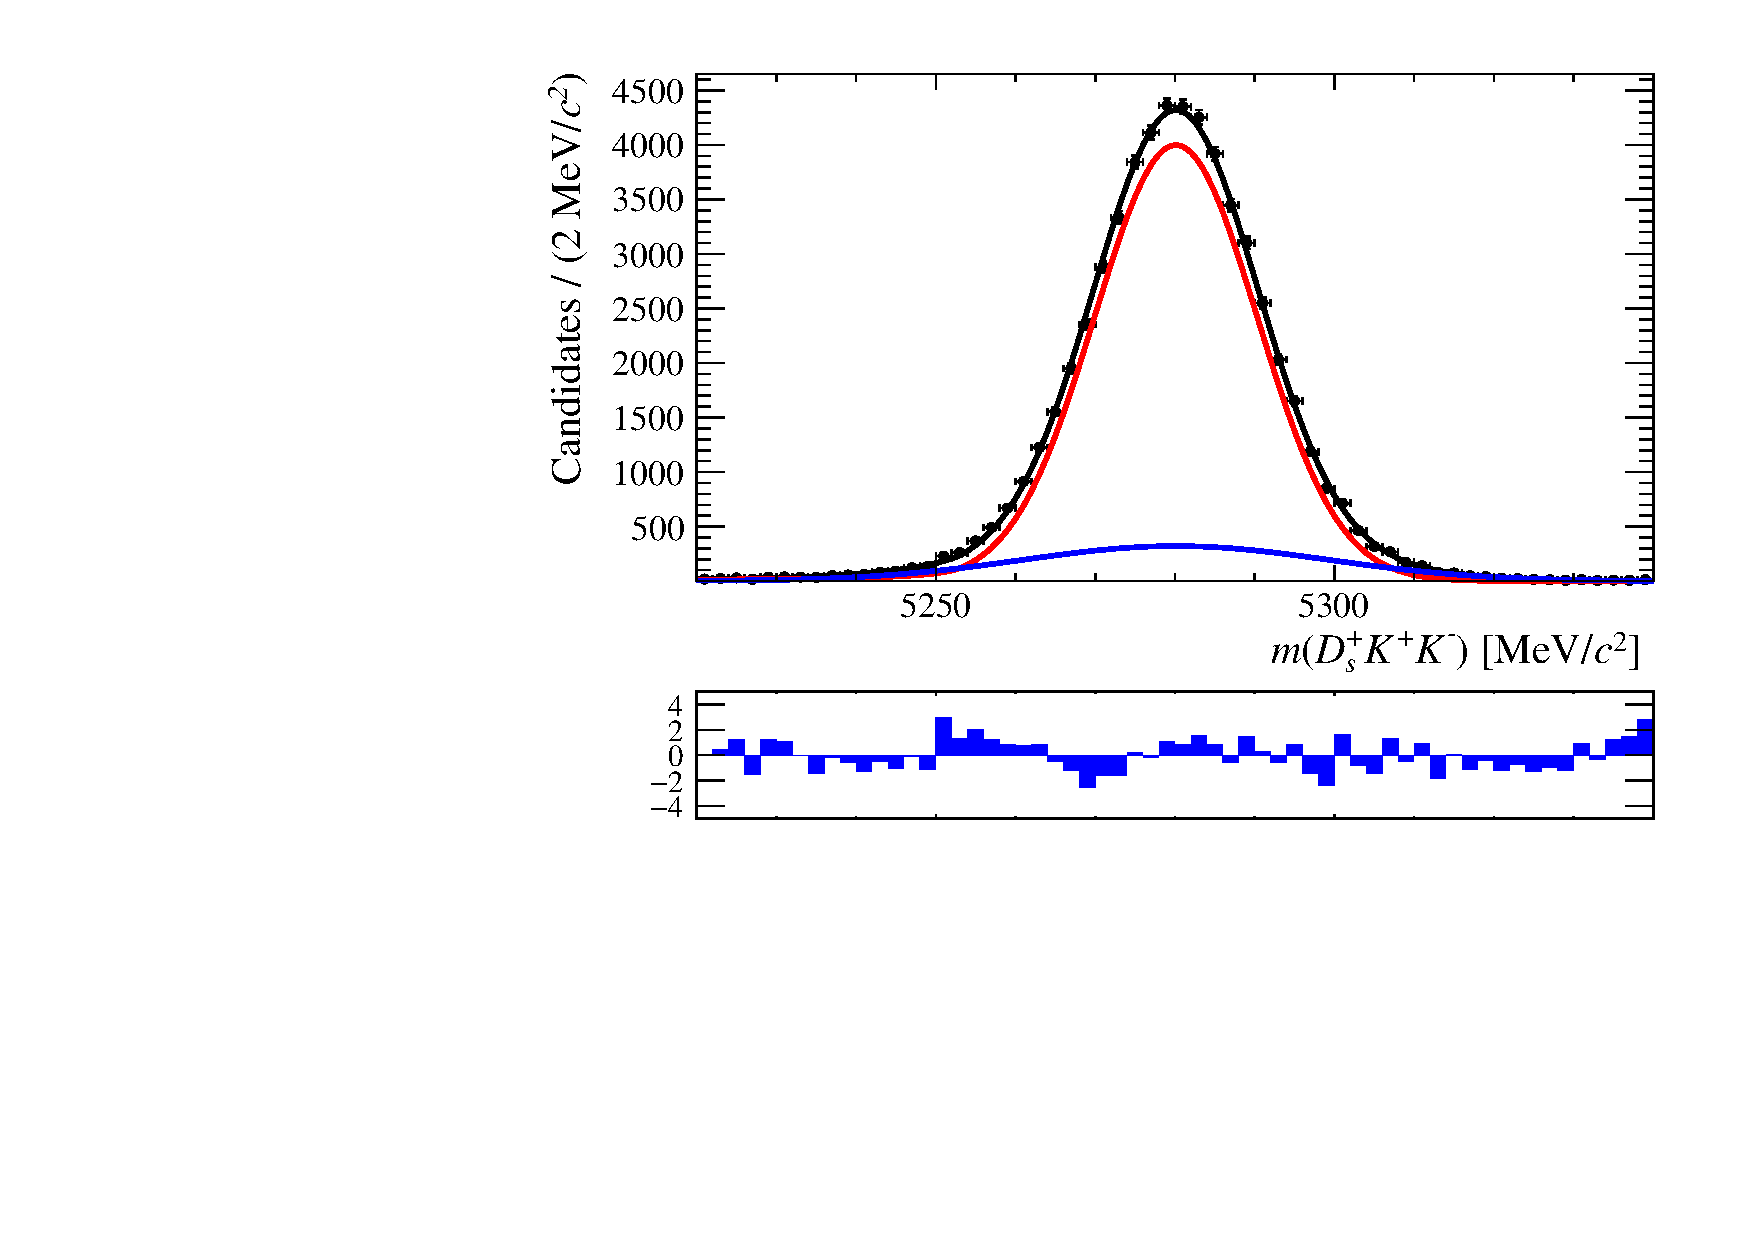
\includegraphics[width=0.48\textwidth]{figs/B2DsKK/Plot_Signal_Fit_All_B2DsKK_Ds2KKPi.pdf}
        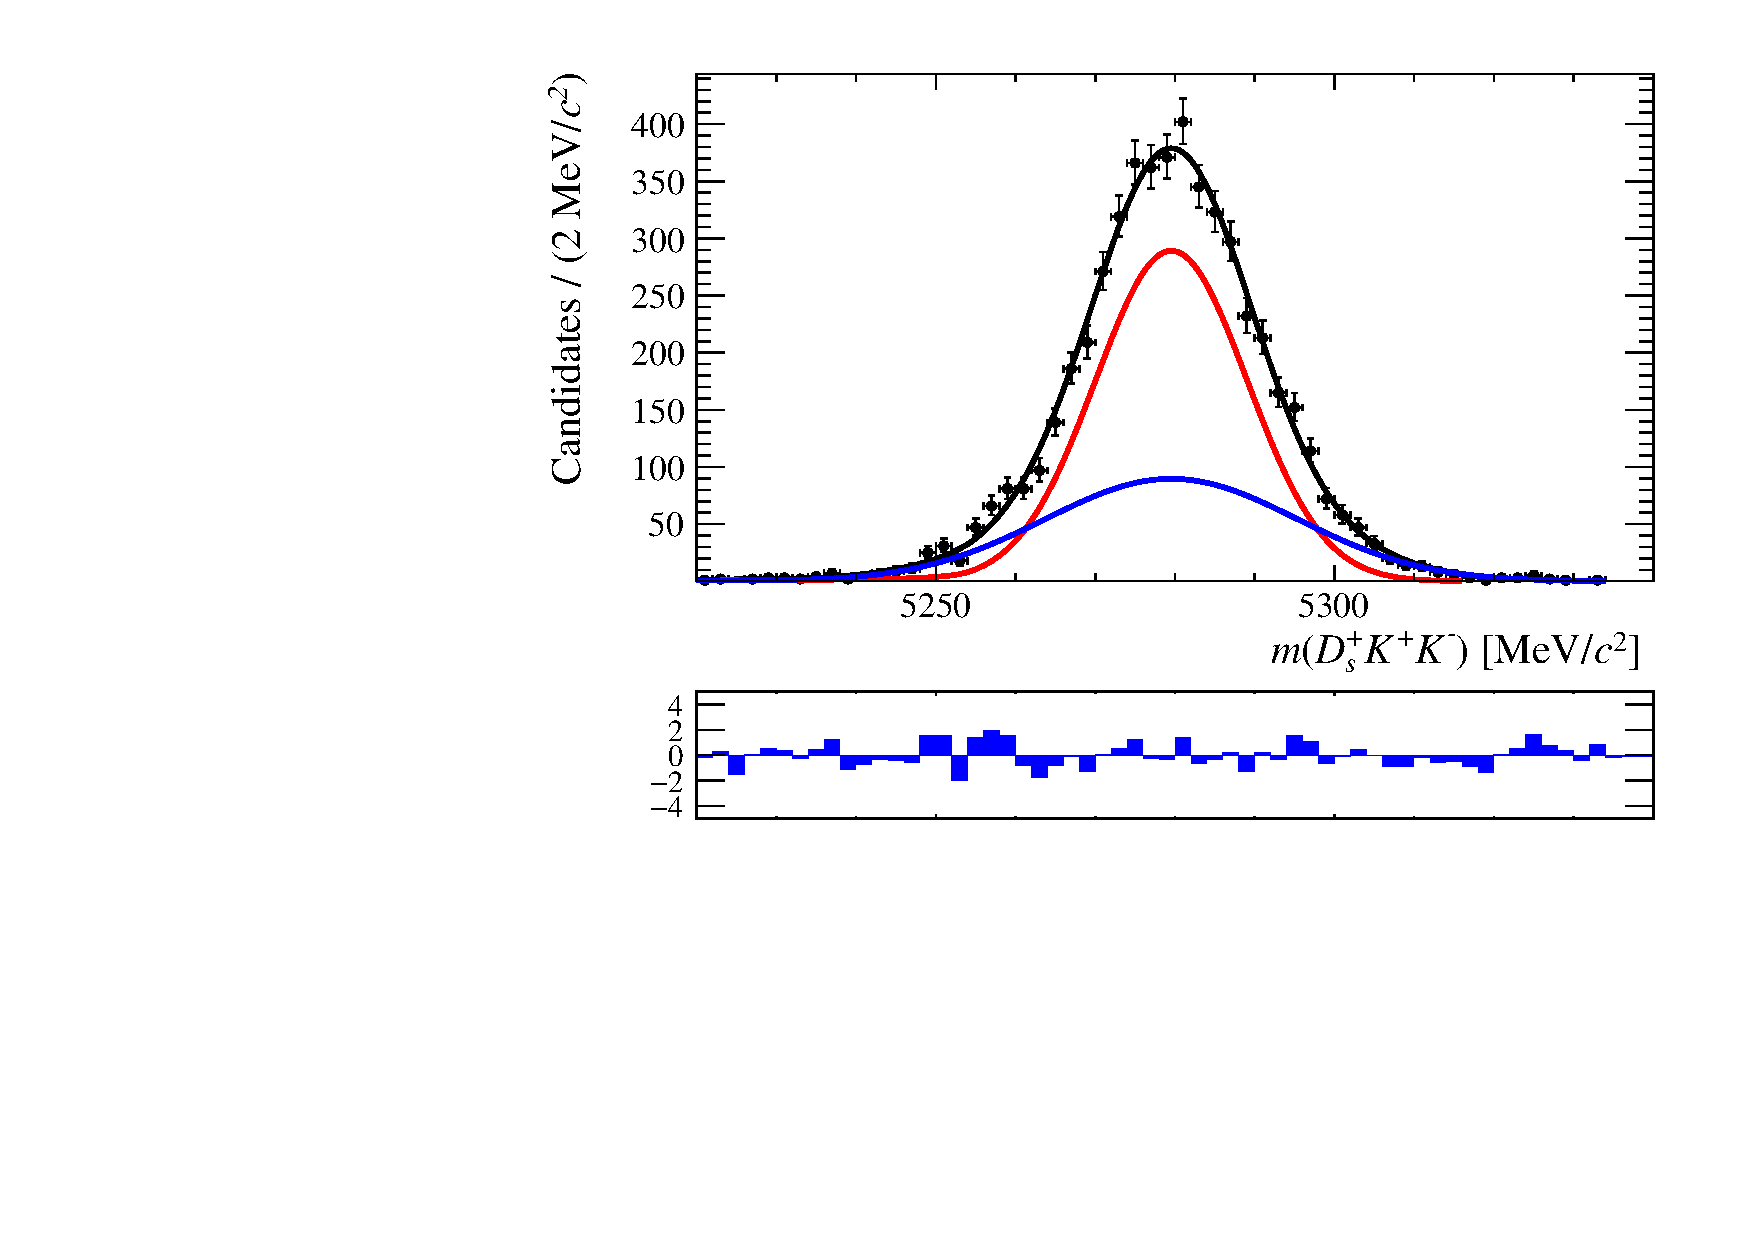
\includegraphics[width=0.48\textwidth]{figs/B2DsKK/Plot_Signal_Fit_All_B2DsD0_Ds2KKPi.pdf}
    \end{subfigure}\\
    \caption{Invariant mass fits to signal (left) and normalisation (right) channel simulation samples.}
    \label{fig:B2DsKK_signal_fits}   
\end{figure}
%%%%%%%%%%%%%%%%%%%%%%%%%%%%%%%%%%%%%%%%%%%%%%%%%%%%%%%%%%


\subsection{Partially reconstructed backgrounds}
\label{sec:B2DsKK_partrecocomps}

Partially reconstructed decays are those in which the five final state particles combined in the signal mode are only a subset of a background mode's final state.
Decays of \bquark-hadrons can contribute at lower invariant masses below the signal peak when one or more the decay products have not been reconstructed. 
For decays to contribute within the fitted \Bp invariant mass window, the particle or particles that have not been reconstructed must be fairly low-momentum (soft) such that the invariant mass of the remaining particles is large. Accurate parametrisation of these contributions is vital as many of the distributions extend close to or within the range of the signal distribution. Incorrectly attributing these decays to the signal component could lead to the incorrect branching fraction being measured. 

\subsubsection{Backgrounds to the normalisation channel}
\label{sec:B2DsKK_norm_partreco}

The low invariant mass region of the \Dsp\Dzb spectrum is populated by decays of \Bp mesons to combinations of \D and excited \D mesons. These \Dstarzb and \Dss mesons decay strongly to a ground state \Dzb or \Dsp meson and a soft pion or photon. The branching fractions for these decays are listed in Table~\ref{tab:dstar_BFs}.


%%%%%%%%%%%%%%%%%%%%%%%%%%%%%%%%%%%%%%%%%%%%%%%%%%%%%%%%%% 
\begin{table}[h]
\centering
\begin{tabular}{ l c }

\hline
Decay                           & Branching fraction \\ 
\hline
\decay{\Dstarzb}{\Dzb\Pgamma}   &   $(64.7\pm0.9)\%$ \\
\decay{\Dstarzb}{\Dzb\piz}      &   $(35.3\pm0.9)\%$ \\
\decay{\Dssp}{\Dsp\Pgamma}      &   $(93.5\pm0.7)\%$ \\
\decay{\Dssp}{\Dsp\piz}         &    $(5.8\pm0.7)\%$ \\
\hline

\end{tabular}  
\caption{Branching fractions for excited charm mesons \cite{PDG2016}. } 
\label{tab:dstar_BFs}
\end{table}
%%%%%%%%%%%%%%%%%%%%%%%%%%%%%%%%%%%%%%%%%%%%%%%%%%%%%%%%%% 

The excited charm mesons \Dstarzb and \Dss {\color{Red}(be more specific)} are vector ($J^{P} = 1^{-}$) mesons. The partially reconstructed invariant mass of the \Dsp and \Dzb mesons, $m(\Dsp\Dzb)$, varies depending on the spin of the missed particle.
Analytical PDFs are used to account for the spin and mass of the missing particle. These PDFs have been used to describe other partially reconstructed \decay{\B}{\D X} decays investigated by the LHCb collaboration~\cite{LHCb-PAPER-2017-021}. 

\begin{description}
\item \textbf{\decay{\Bp}{(\decay{\Dssp}{\Dsp[\piz]})\Dzb} and \decay{\Bp}{\Dsp(\decay{\Dstarzb}{\Dzb[\piz]})}:} the \piz meson is a pseudo-scalar ($J^{P} = 0^{-}$) particle with a mass $m(\piz) = 134.9766 \pm 0.0006 \mevcc$. The partially reconstructed invariant mass distribution $m(\Dsp\Dzb)$ can be described by a parabola convolved with a Gaussian resolution function. The parabola does not extend beyond kinematic endpoints defined by the parameters $a$ and $b$ and has a minimum in the centre 
\begin{equation}
f(m|a,b,\sigma,\xi, \delta) = \int_{a}^{b}\left(\mu-\frac{a+b}{2}\right)^{2} \left( \frac{1-\xi}{b-a}\mu + \frac{b\xi-a}{b-a} \right) e^{-\frac{-(\mu-(m-\delta))^{2}}{2\sigma^{2}}} d\mu.
\end{equation} 

Here, $\sigma$ is the width of the resolution Gaussian and $\delta$ allows the function to be offset in invariant mass. The parameter $\xi$ introduces the freedom for the two sides of the parabola to have difference heights, achieved by multiplying the parabola by a line whose slope is depends on $\xi$. The resulting function is a double peaked structure shown in Fig.~\ref{fig:B2DsPhi_DsD0_partreco}.   
The parameters $a$ and $b$ are calculated from the kinematics of the \decay{\Bp}{(\decay{\Dssp}{\Dsp\piz})\Dzb} and \decay{\Bp}{\Dsp(\decay{\Dstarzb}{\Dzb\piz})} decays respectively, and are listed in Table~\ref{tab:DsKK_pi0_a_and_b}.

\end{description}

\begin{description}

%%%%%%%%%%%%%%%%%%%%%%%%%%%%%%%%%%%%%%%%%%%%%%%%%%%%%%%%%% 
\begin{table}[h]
\centering
\begin{tabular}{ l c c }

\hline
Mode                                              & $a$ (\mevcc)       & $b$ (\mevcc)   \\ 
\hline
\decay{\Bp}{(\decay{\Dssp}{\Dsp[\piz]})\Dzb}      & 5051.4            &  5132.9       \\
\decay{\Bp}{\Dsp(\decay{\Dstarzb}{\Dzb[\piz]})}   & 5051.5            &  5128.6       \\
\hline
\end{tabular}  
\caption{Kinematic endpoints for the partially reconstructed \decay{\Bp}{(\decay{\Dssp}{\Dsp\piz})\Dzb} and \decay{\Bp}{\Dsp(\decay{\Dstarzb}{\Dzb\piz})} decays.} 
\label{tab:DsKK_pi0_a_and_b}
\end{table}
%%%%%%%%%%%%%%%%%%%%%%%%%%%%%%%%%%%%%%%%%%%%%%%%%%%%%%%%%%


\item \textbf{\decay{\Bp}{(\decay{\Dssp}{\Dsp[\Pgamma]})\Dzb} and \decay{\Bp}{\Dsp(\decay{\Dstarzb}{\Dzb[\Pgamma]})}:} the \Pgamma boson is a massless vector ($J^{P} = 1^{-}$) particle. The partially reconstructed $m(\Dsp\Dzb)$ invariant mass is also described by a parabola convolved with a Gaussian resolution function. The parabola does not extend beyond the endpoints $a$ and $b$, and has a maximum in the centre   
\begin{equation}
f(m|a,b,\sigma,\xi, \delta) = \int_{a}^{b} -(\mu-a)(\mu-b)\left( \frac{1-\xi}{b-a}\mu + \frac{b\xi-a}{b-a} \right) e^{-\frac{-(\mu-(m-\delta))^{2}}{2\sigma^{2}}} d\mu.
\end{equation}
Again $\sigma$, $\delta$ and $\xi$ control the width, offset and relative heights of two sides of the parabola. The resulting function is a broad single peak shown in Fig.~\ref{fig:B2DsKK_part_reco_backgrounds}.

\end{description}

%%%%%%%%%%%%%%%%%%%%%%%%%%%%%%%%%%%%%%%%%%%%%%%%%%%%%%%%%% 
\begin{table}[h]
\centering
\begin{tabular}{ l c c }

\hline
Mode                                                 & $a$ (\mevcc)      & $b$ (\mevcc)  \\ 
\hline
\decay{\Bp}{(\decay{\Dssp}{\Dsp[\Pgamma]})\Dzb}      & 4976.7            &  5213.1       \\
\decay{\Bp}{\Dsp(\decay{\Dstarzb}{\Dzb[\Pgamma]})}   & 4970.1            &  5216.1       \\
\hline
\end{tabular}  
\caption{Kinematic endpoints for the partially reconstructed \decay{\Bp}{(\decay{\Dssp}{\Dsp\Pgamma})\Dzb} and \decay{\Bp}{\Dsp(\decay{\Dstarzb}{\Dzb\Pgamma})} decays.} 
\label{tab:DsKK_gamma_a_and_b}
\end{table}
%%%%%%%%%%%%%%%%%%%%%%%%%%%%%%%%%%%%%%%%%%%%%%%%%%%%%%%%%%


%%%%%%%%%%%%%%%%%%%%%%%%%%%%%%%%%%%%%%%%%%%%%%%%%%%%%%%%%%
\begin{figure}[!h]
    \centering
    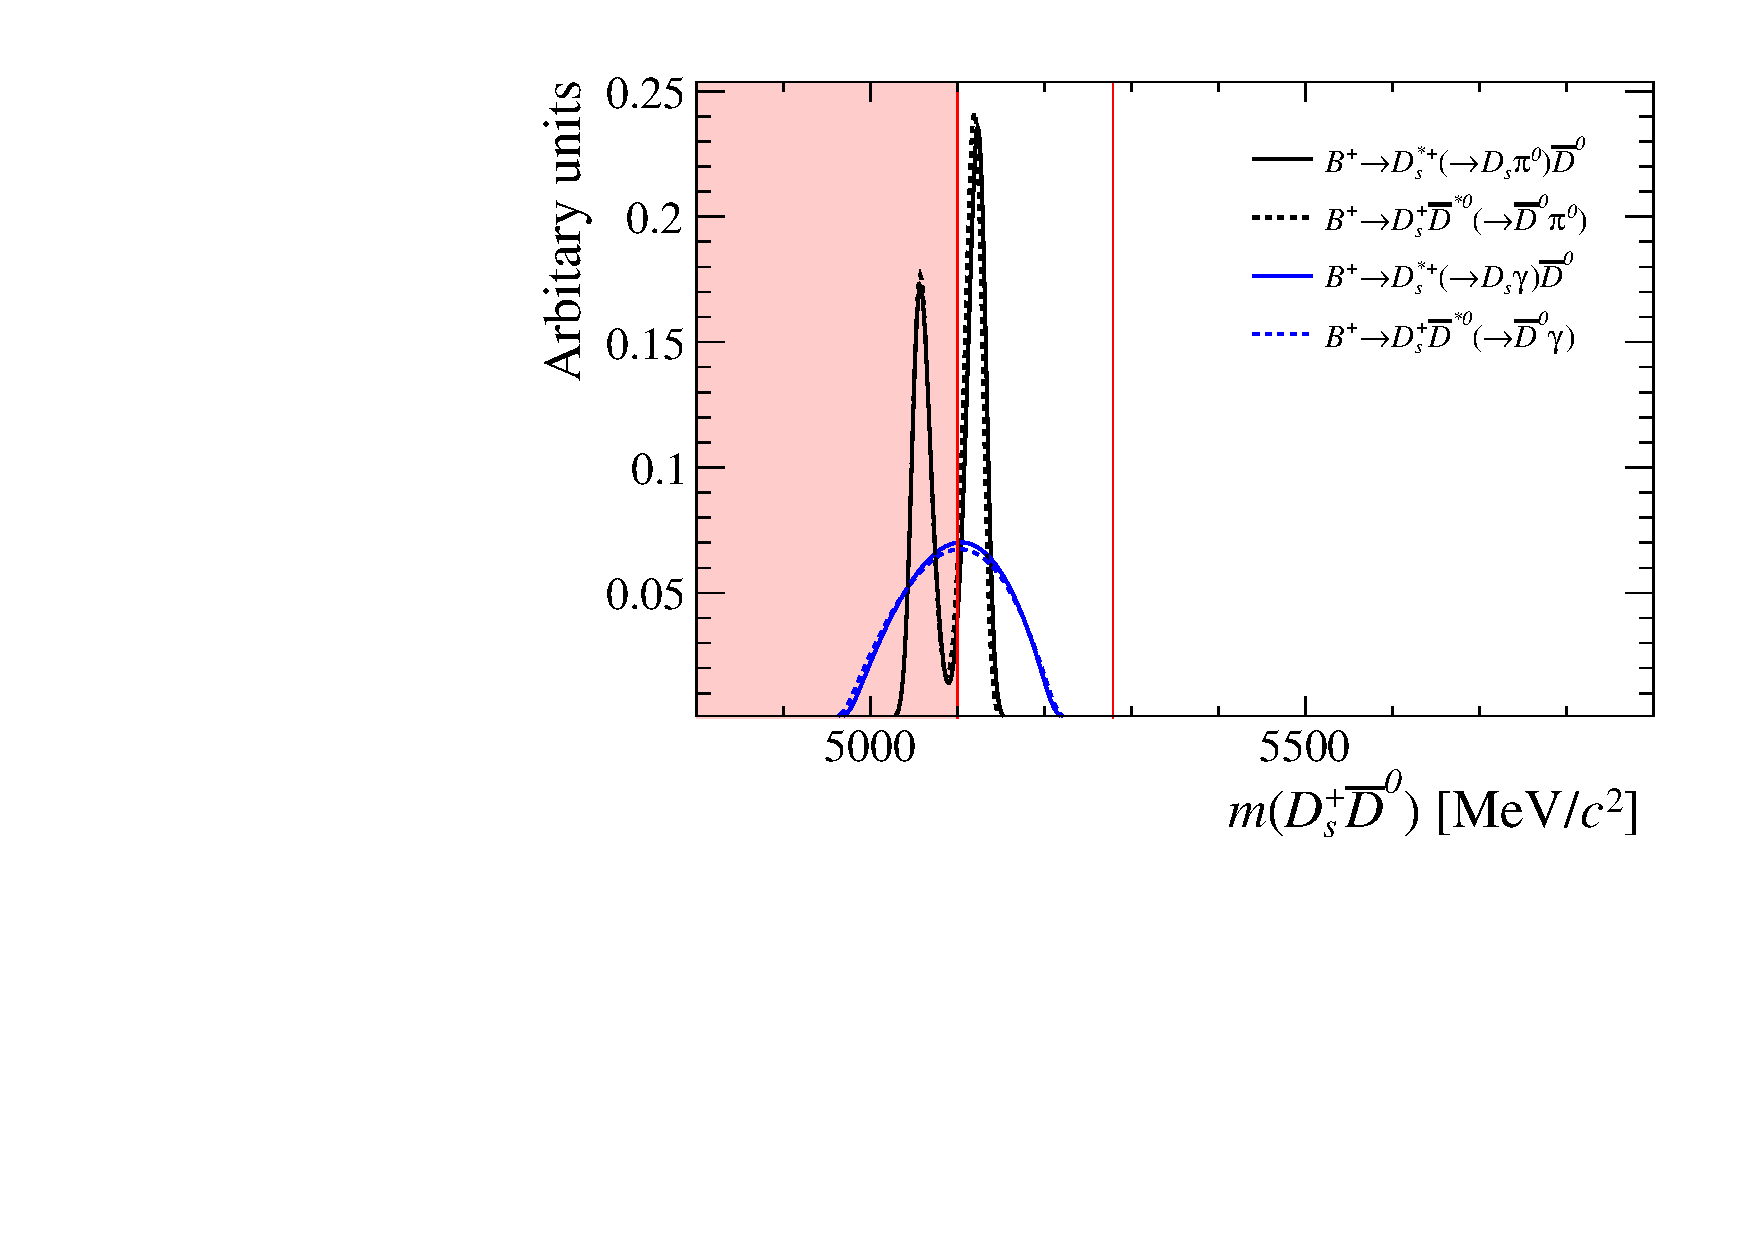
\includegraphics[width=0.80\textwidth]{figs/B2DsKK/B2DsKK_DsD0_part_reco_Shapes.pdf}
    \caption{Partially reconstructed \decay{\Bp}{\Dssp\Dzb} and \decay{\Bp}{\Dsp\Dstarzb} PDFs as described in Sec.~\ref{sec:B2DsKK_norm_partreco}. The range below $5100\mevcc$ (highlighted in red) is not included in the fit range, but included to shown the full PDF distributions. The \Bp meson mass is represented by a vertical line.} 
    \label{fig:B2DsPhi_DsD0_partreco}   
\end{figure}
%%%%%%%%%%%%%%%%%%%%%%%%%%%%%%%%%%%%%%%%%%%%%%%%%%%%%%%%%%





\subsubsection{Backgrounds to the signal channel}

The signal channel receives contributions at low invariant mass from a number of different decays. 
All modes considered involve a \Bs or \Bz meson decay in which one or more soft decay products have not been reconstructed.

\begin{description}
\item \decay{\Bsb}{\Dsp\Km\Kstarz}: this decay can form a background to the \decay{\Bp}{\Dsp\Kp\Km} signal when a soft pion from the \decay{\Kstarz}{\Kp\pim} decay is not reconstructed. The $\Km\Kstarz$ is modelled as originating from the $a_1(1260)$ resonance. This resonance has a width of $250-600$ MeV~\cite{PDG2016}, allowing it to decay to $\Km\Kstarz$ even though it's pole mass is below the $\Km\Kstarz$ threshold.
The PDF for this background is determined from a sample of fully reconstructed simulated events that have been processed using the same procedure as the signal decays. The PDF is created using a kernel estimation technique~\cite{Cranmer:2000du} implemented in the \texttt{RooKeysPDF} class within \roofit. The resulting PDF is shown in Fig.~\ref{fig:B2DsKK_part_reco_backgrounds_DsKKstar}.
\end{description}

%%%%%%%%%%%%%%%%%%%%%%%%%%%%%%%%%%%%%%%%%%%%%%%%%%%%%%%%%%
\begin{figure}[!h]
    \centering
    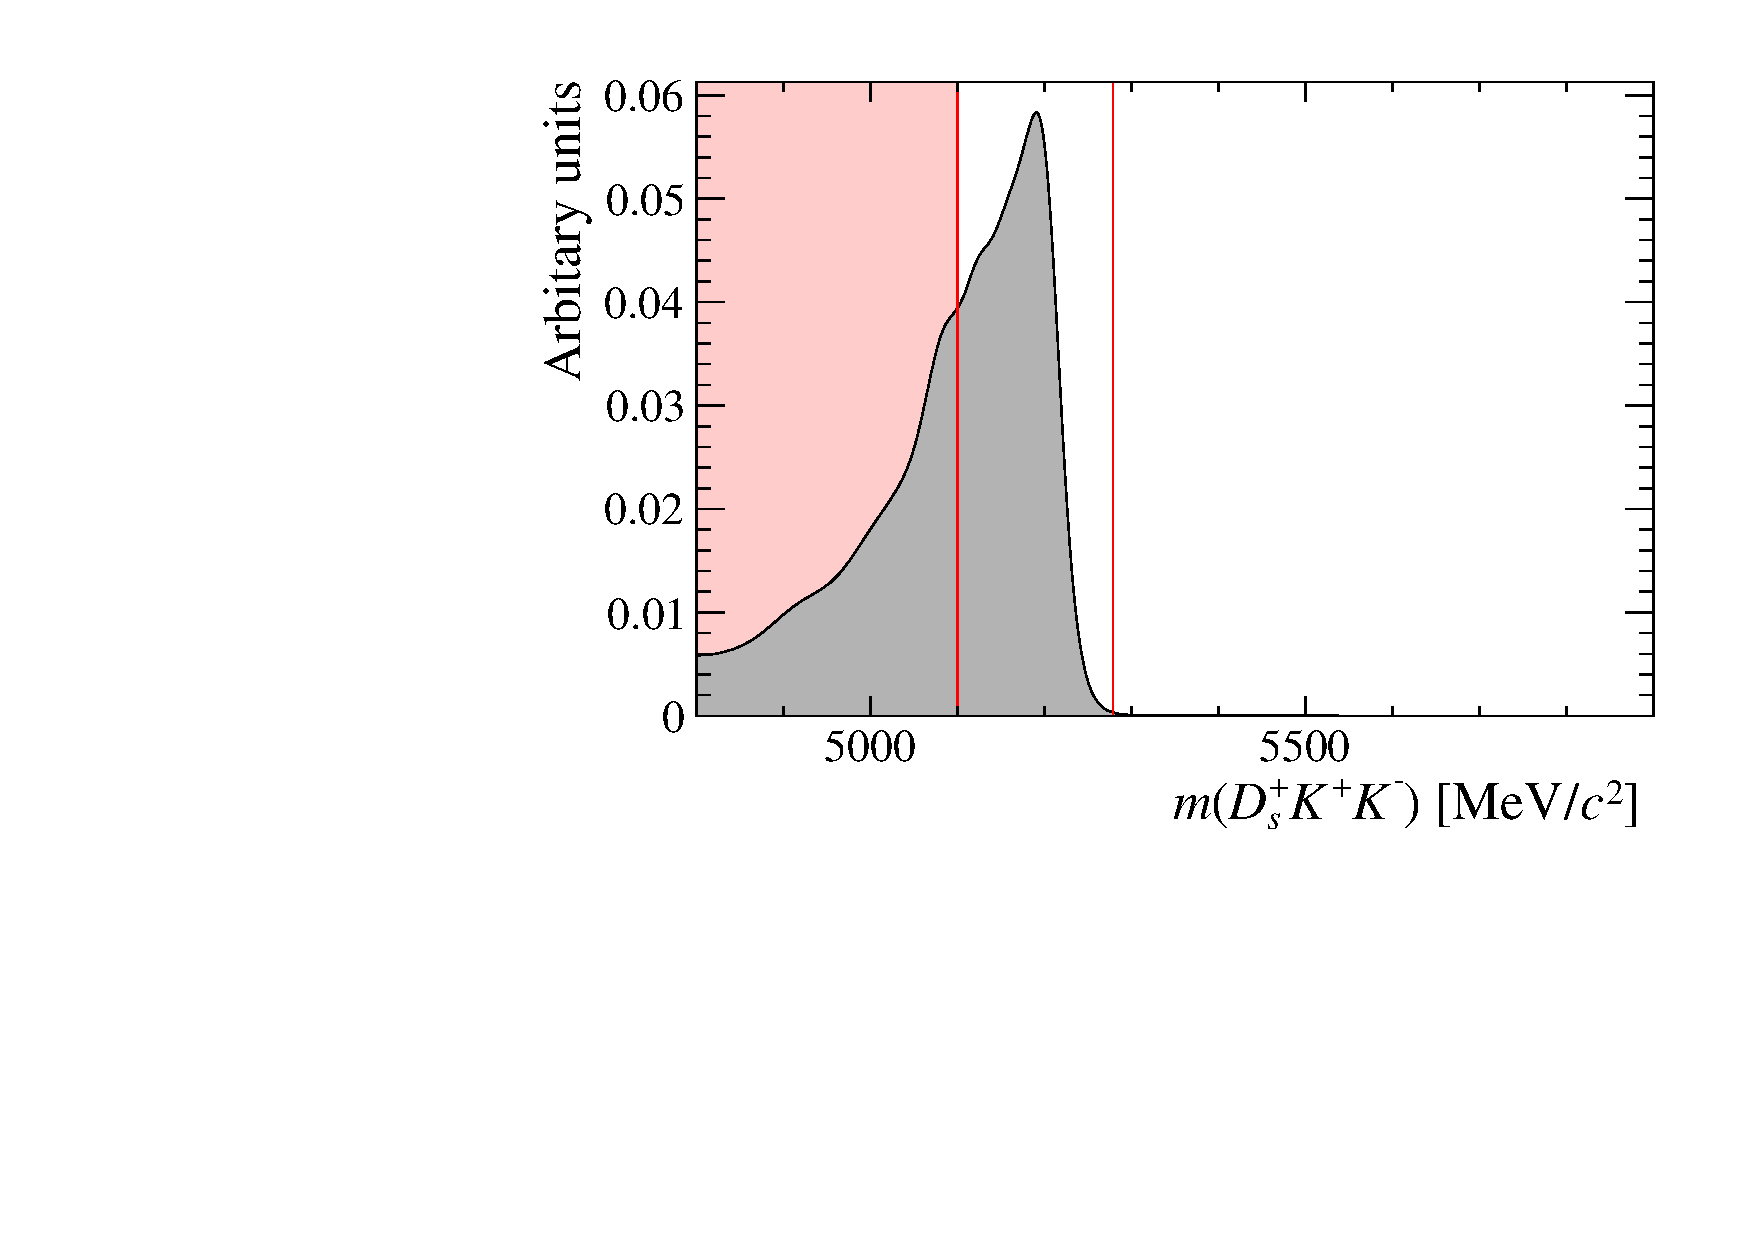
\includegraphics[width=0.49\textwidth]{figs/B2DsKK/Bs2Dsa1_4800_5900_Shape.pdf}
    \caption{Partially reconstructed \decay{\Bsb}{\Dsp\Km\Kstarz} mass shape.}
    \label{fig:B2DsKK_part_reco_backgrounds_DsKKstar}   
\end{figure}
%%%%%%%%%%%%%%%%%%%%%%%%%%%%%%%%%%%%%%%%%%%%%%%%%%%%%%%%%%

\begin{description}
\item \decay{\Bsb}{\Dssp\Km\Kstarz}: similarly this decay can form a background at low invariant mass when a soft neutral particle is not reconstructed in the \decay{\Dssp}{\Dsp X} decay in addition to the pion from the \Kstarz. This PDF is also determined using the \texttt{RooKeysPDF} class and shown in Fig.~\ref{fig:B2DsKK_part_reco_backgrounds_DssKKstar}.
\end{description}

%%%%%%%%%%%%%%%%%%%%%%%%%%%%%%%%%%%%%%%%%%%%%%%%%%%%%%%%%%
\begin{figure}[!h]
    \centering
    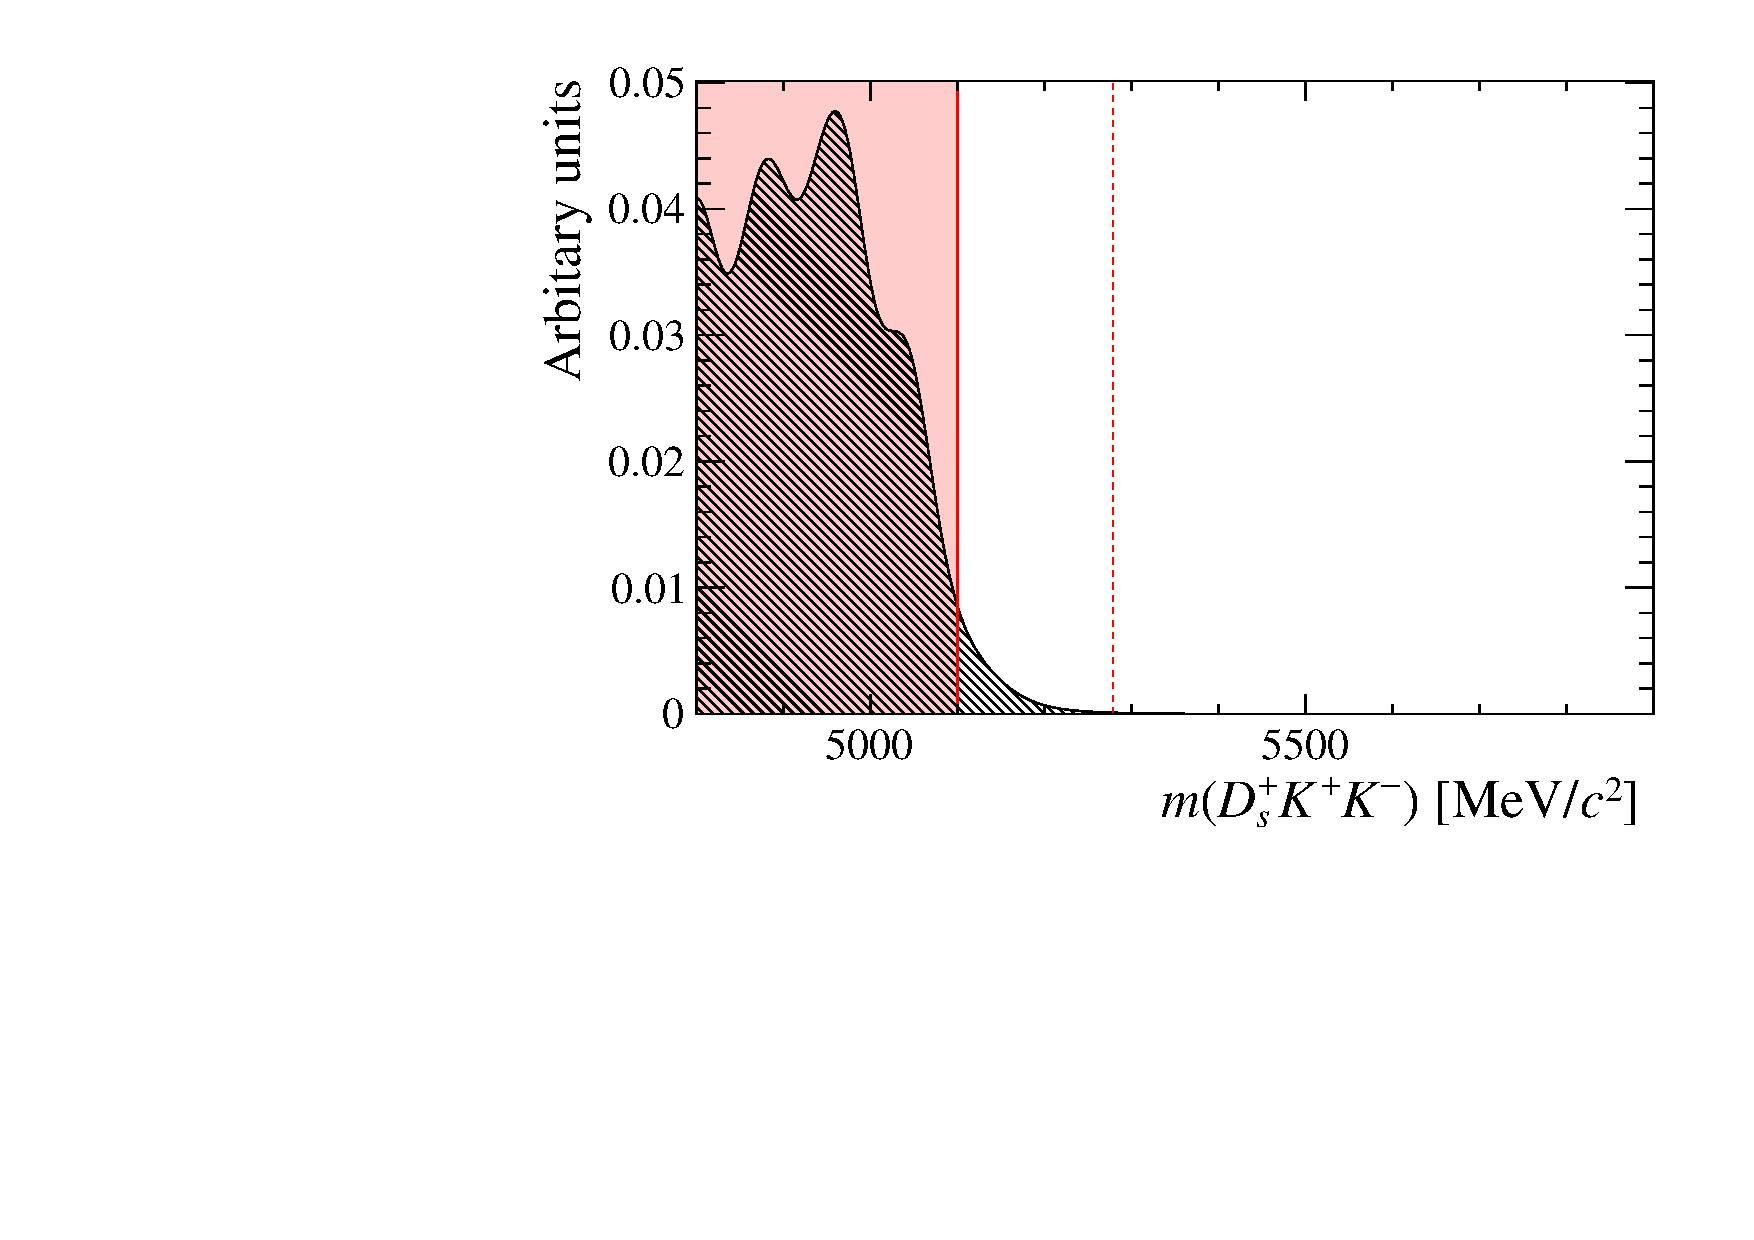
\includegraphics[width=0.49\textwidth]{figs/B2DsKK/Bs2DsstKKst_4800_5900_Shape.pdf}
    \caption{Partially reconstructed \decay{\Bsb}{\Dssp\Km\Kstarz} mass shape.}
    \label{fig:B2DsKK_part_reco_backgrounds_DssKKstar}   
\end{figure}
%%%%%%%%%%%%%%%%%%%%%%%%%%%%%%%%%%%%%%%%%%%%%%%%%%%%%%%%%%

\begin{description}
\item \decay{\Bsb}{\Dsp\Dsm}: this decay can form a background to the signal when a pion is missed from either of the \Dsp decays. This requires both \Dsp mesons to decay to the \decay{\Dsp}{\Kp\Km\pip} final state. 
%Due to the large phase space of \decay{\Dsp}{\Kp\Km\pip} decays, the pion is not as soft as in the previous background modes. 
%Therefore this background only becomes significant at smaller invariant masses as shown in Fig.~\ref{fig:B2DsKK_part_reco_backgrounds}. 
Therefore this background becomes significant at smaller invariant masses as shown in Fig.~\ref{fig:B2DsKK_part_reco_backgrounds_DsDs}. 
This PDF is similarly determined by creating a kernel estimation of fully-reconstructed simulated events passing the signal selection.  
\end{description}

%%%%%%%%%%%%%%%%%%%%%%%%%%%%%%%%%%%%%%%%%%%%%%%%%%%%%%%%%%
\begin{figure}[!h]
    \centering
    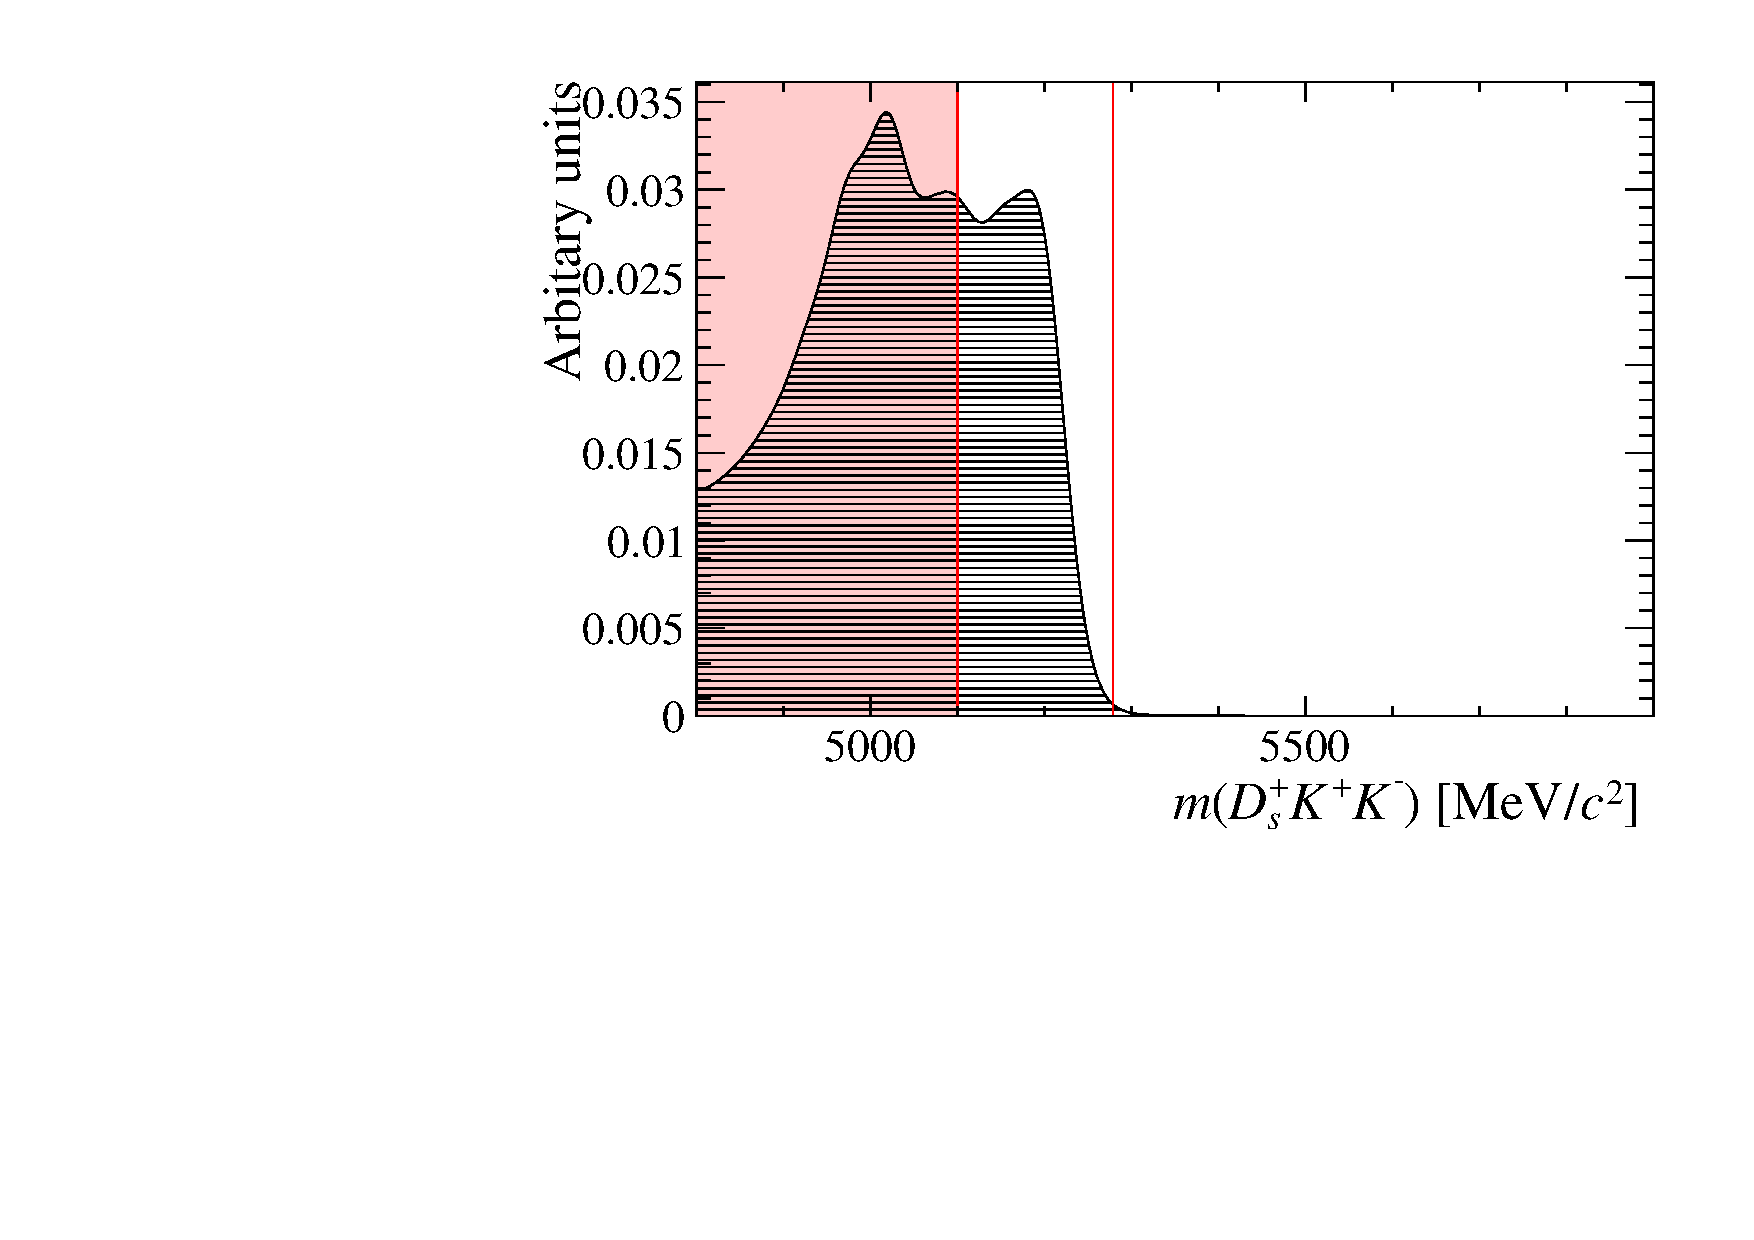
\includegraphics[width=0.49\textwidth]{figs/B2DsKK/Bs2DsDs_4800_5900_Shape.pdf}
    \caption{Partially reconstructed \decay{\Bsb}{\Dsp\Dsm} mass shape.}
    \label{fig:B2DsKK_part_reco_backgrounds_DsDs}   
\end{figure}
%%%%%%%%%%%%%%%%%%%%%%%%%%%%%%%%%%%%%%%%%%%%%%%%%%%%%%%%%%

\begin{description}
\item \decay{\Bzb}{\Dsp\Dm}: this decay can form a background when both the \Dsp and \Dm mesons decay to the \Kpm\Kmp\pipm final state. Due to the similar topology to the \decay{\Bsb}{\Dsp\Dsm} decay, the same PDF determined from simulated events is used, however it is shifted down in mass by 40\mevcc to account for the difference in kinematics.

\item \decay{\Bsb}{\Dssp\Dsm}: similarly this decay can cause a background when both a soft neutral particle is missed from the \decay{\Dssp}{\Dsp X} decay as well as a pion from either of the \Dsp mesons. As such this only has a small contribution within the fit range as shown in Fig.~\ref{fig:B2DsKK_part_reco_backgrounds_DssDs}. 
\end{description}

%%%%%%%%%%%%%%%%%%%%%%%%%%%%%%%%%%%%%%%%%%%%%%%%%%%%%%%%%%
\begin{figure}[!h]
    \centering
    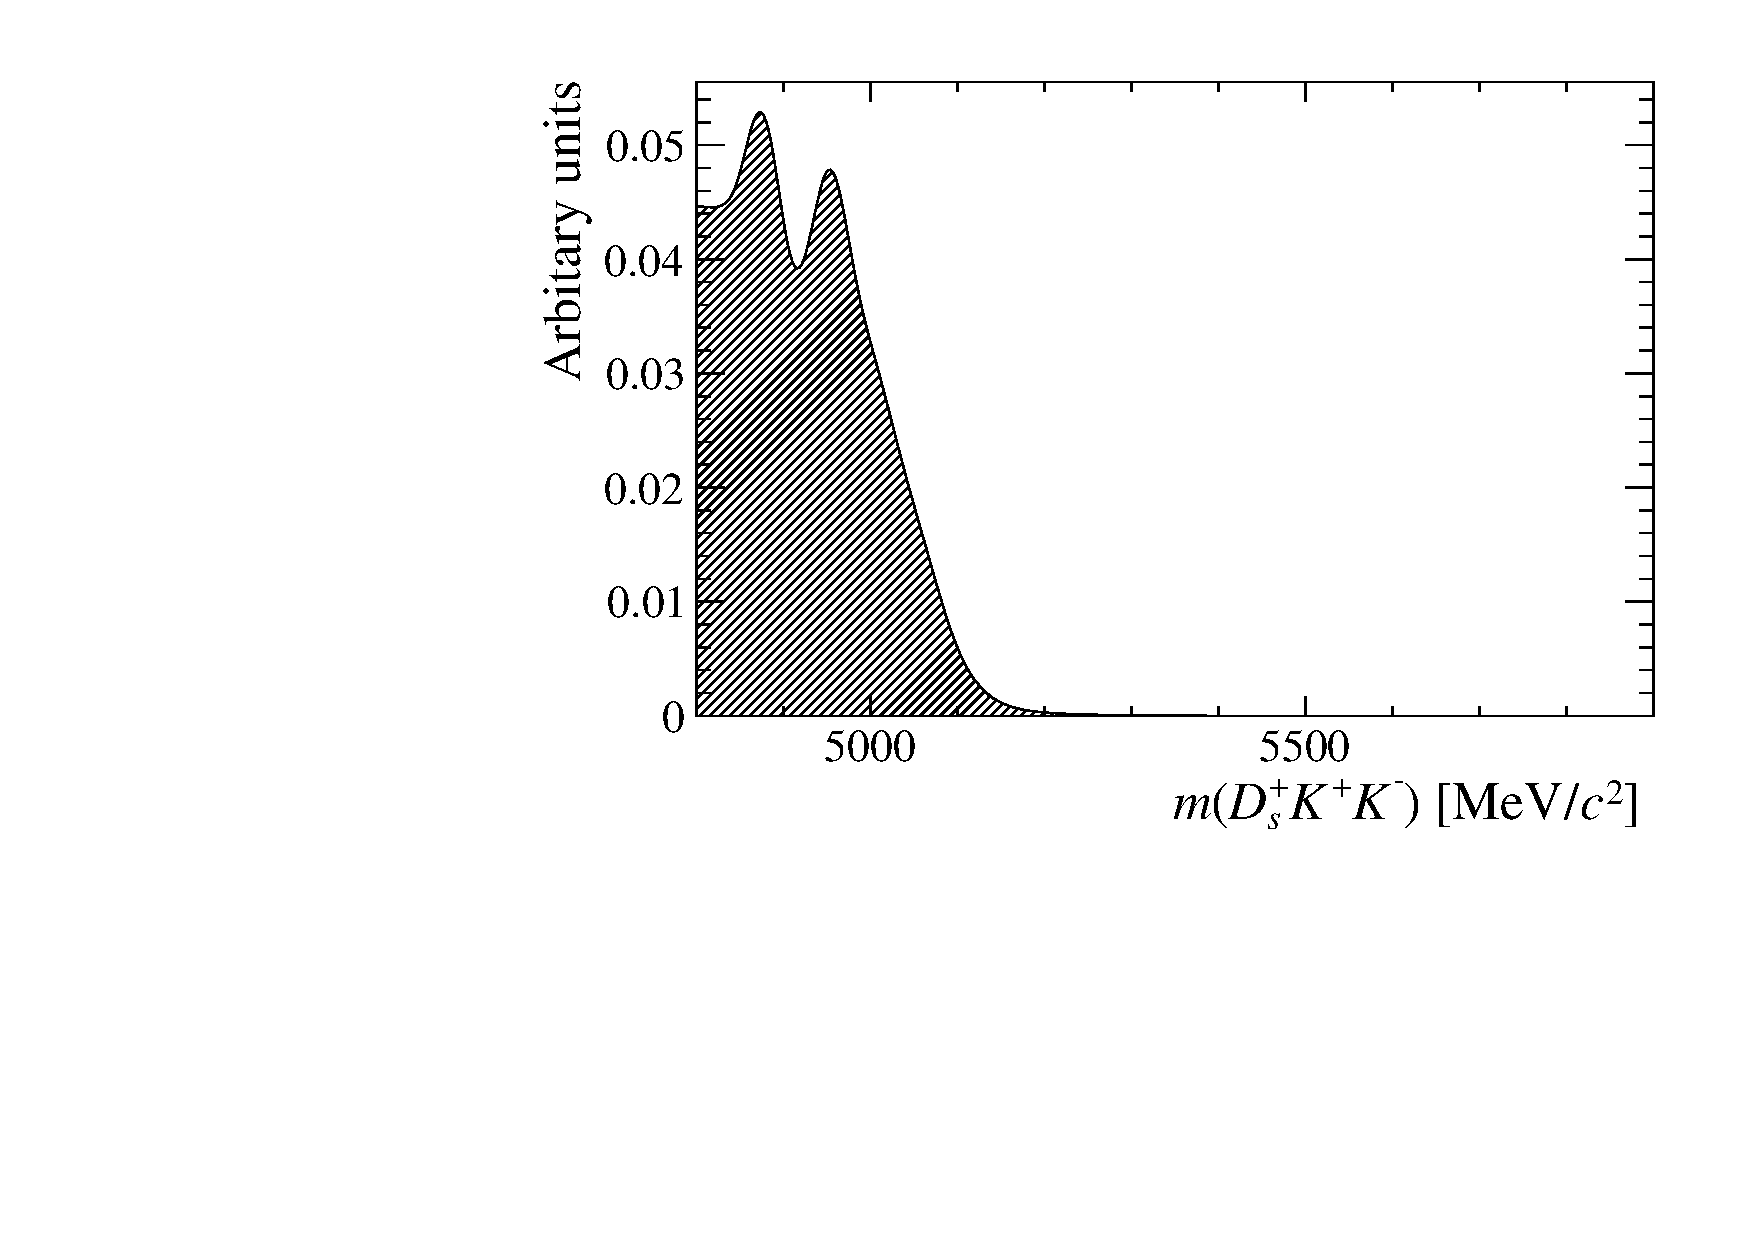
\includegraphics[width=0.49\textwidth]{figs/B2DsKK/Bs2DsstDs_4800_5900_Shape.pdf}
    \caption{Partially reconstructed \decay{\Bsb}{\Dssp\Dsm} mass shape.}
    \label{fig:B2DsKK_part_reco_backgrounds_DssDs}   
\end{figure}
%%%%%%%%%%%%%%%%%%%%%%%%%%%%%%%%%%%%%%%%%%%%%%%%%%%%%%%%%%


All PDFs determined using kernel estimations from simulated events are convolved with a Gaussian distribution to account for difference between the simulations and data. The mean position of the Gaussian is given by a single free parameter $\delta$, allowing these PDF to move slightly high or lower in mass. The width of the Gaussian is increased to account for the difference in resolution between simulation and data.

% %%%%%%%%%%%%%%%%%%%%%%%%%%%%%%%%%%%%%%%%%%%%%%%%%%%%%%%%%%
% \begin{figure}[!h]
%     \centering
%     \begin{subfigure}[t]{0.49\textwidth}
%         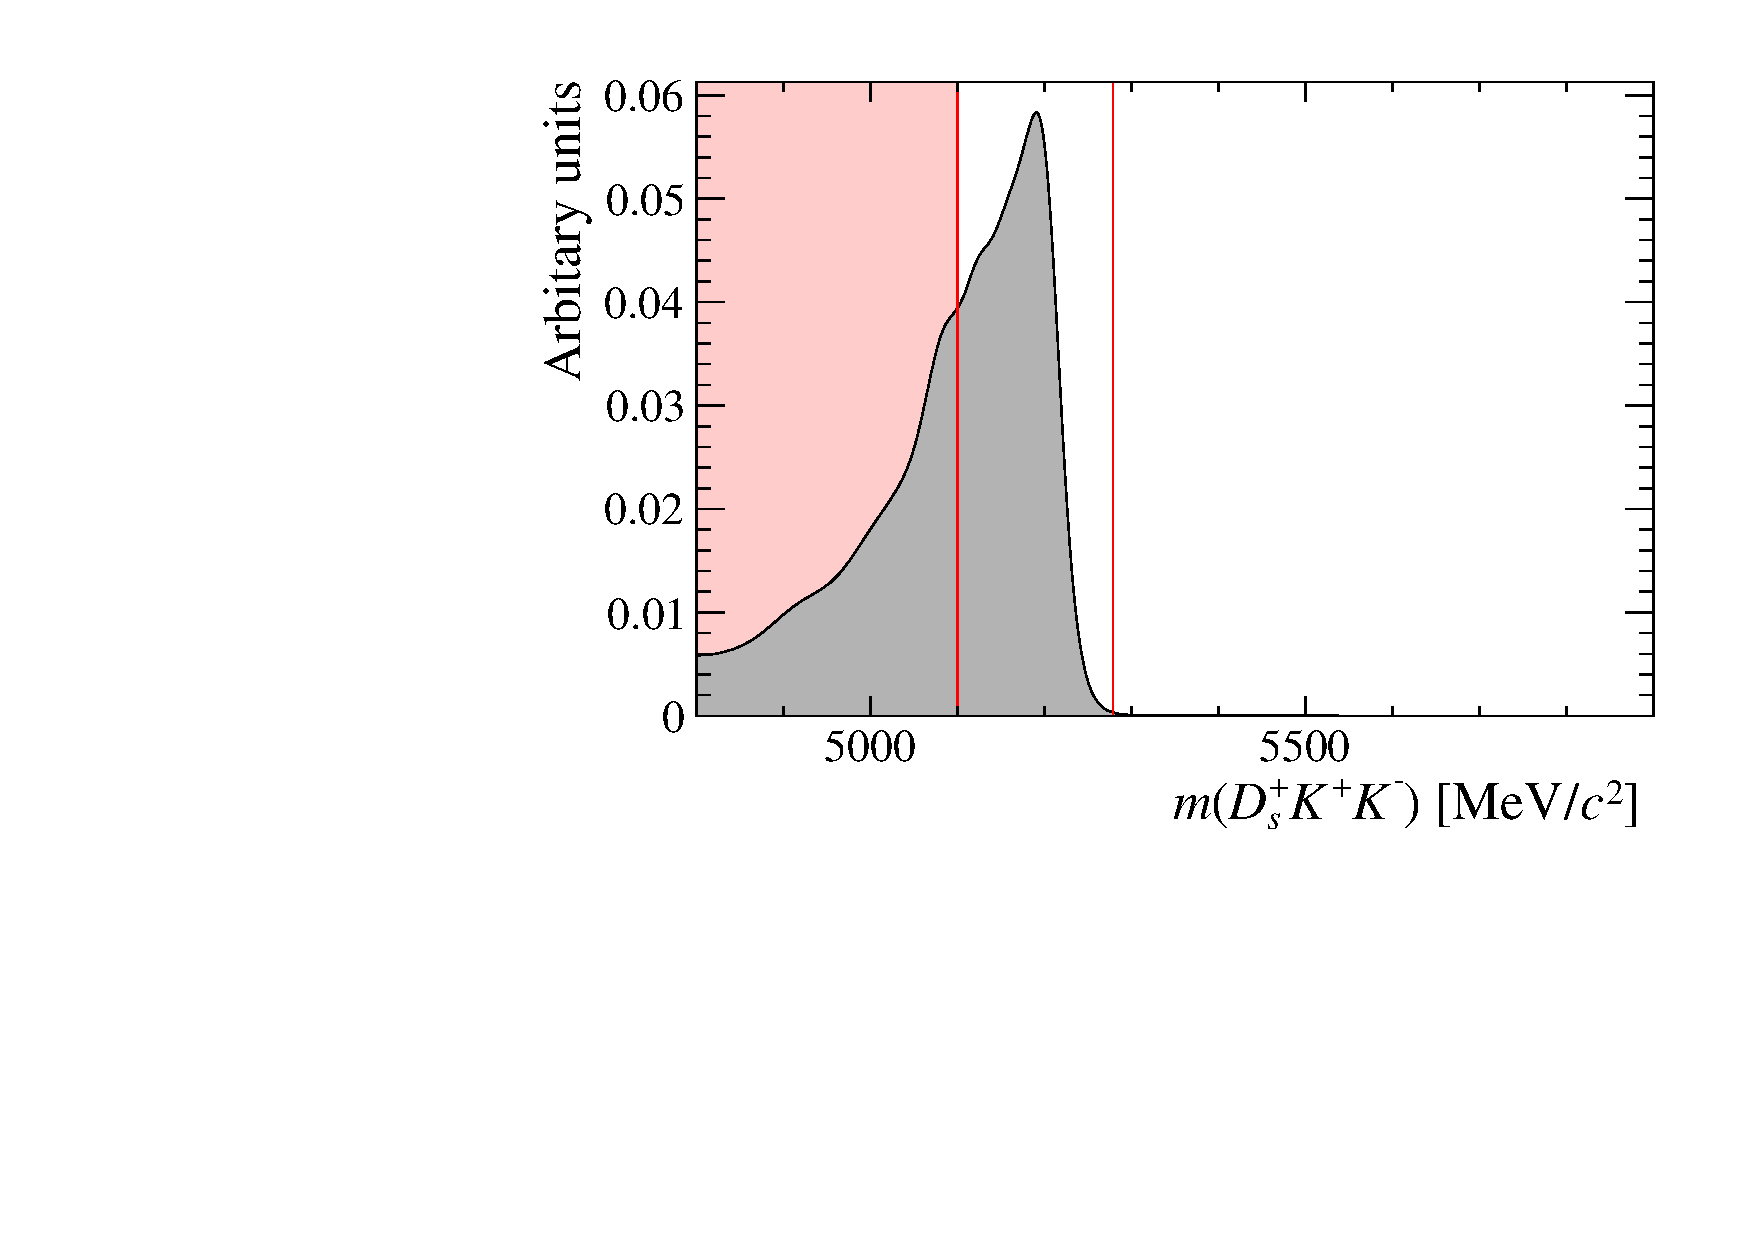
\includegraphics[width=1.0\textwidth]{figs/B2DsKK/Bs2Dsa1_4800_5900_Shape.pdf}
%         \caption{\decay{\Bsb}{\Dsp\Km\Kstarz} }
%     \end{subfigure}
%     \begin{subfigure}[t]{0.49\textwidth}
%         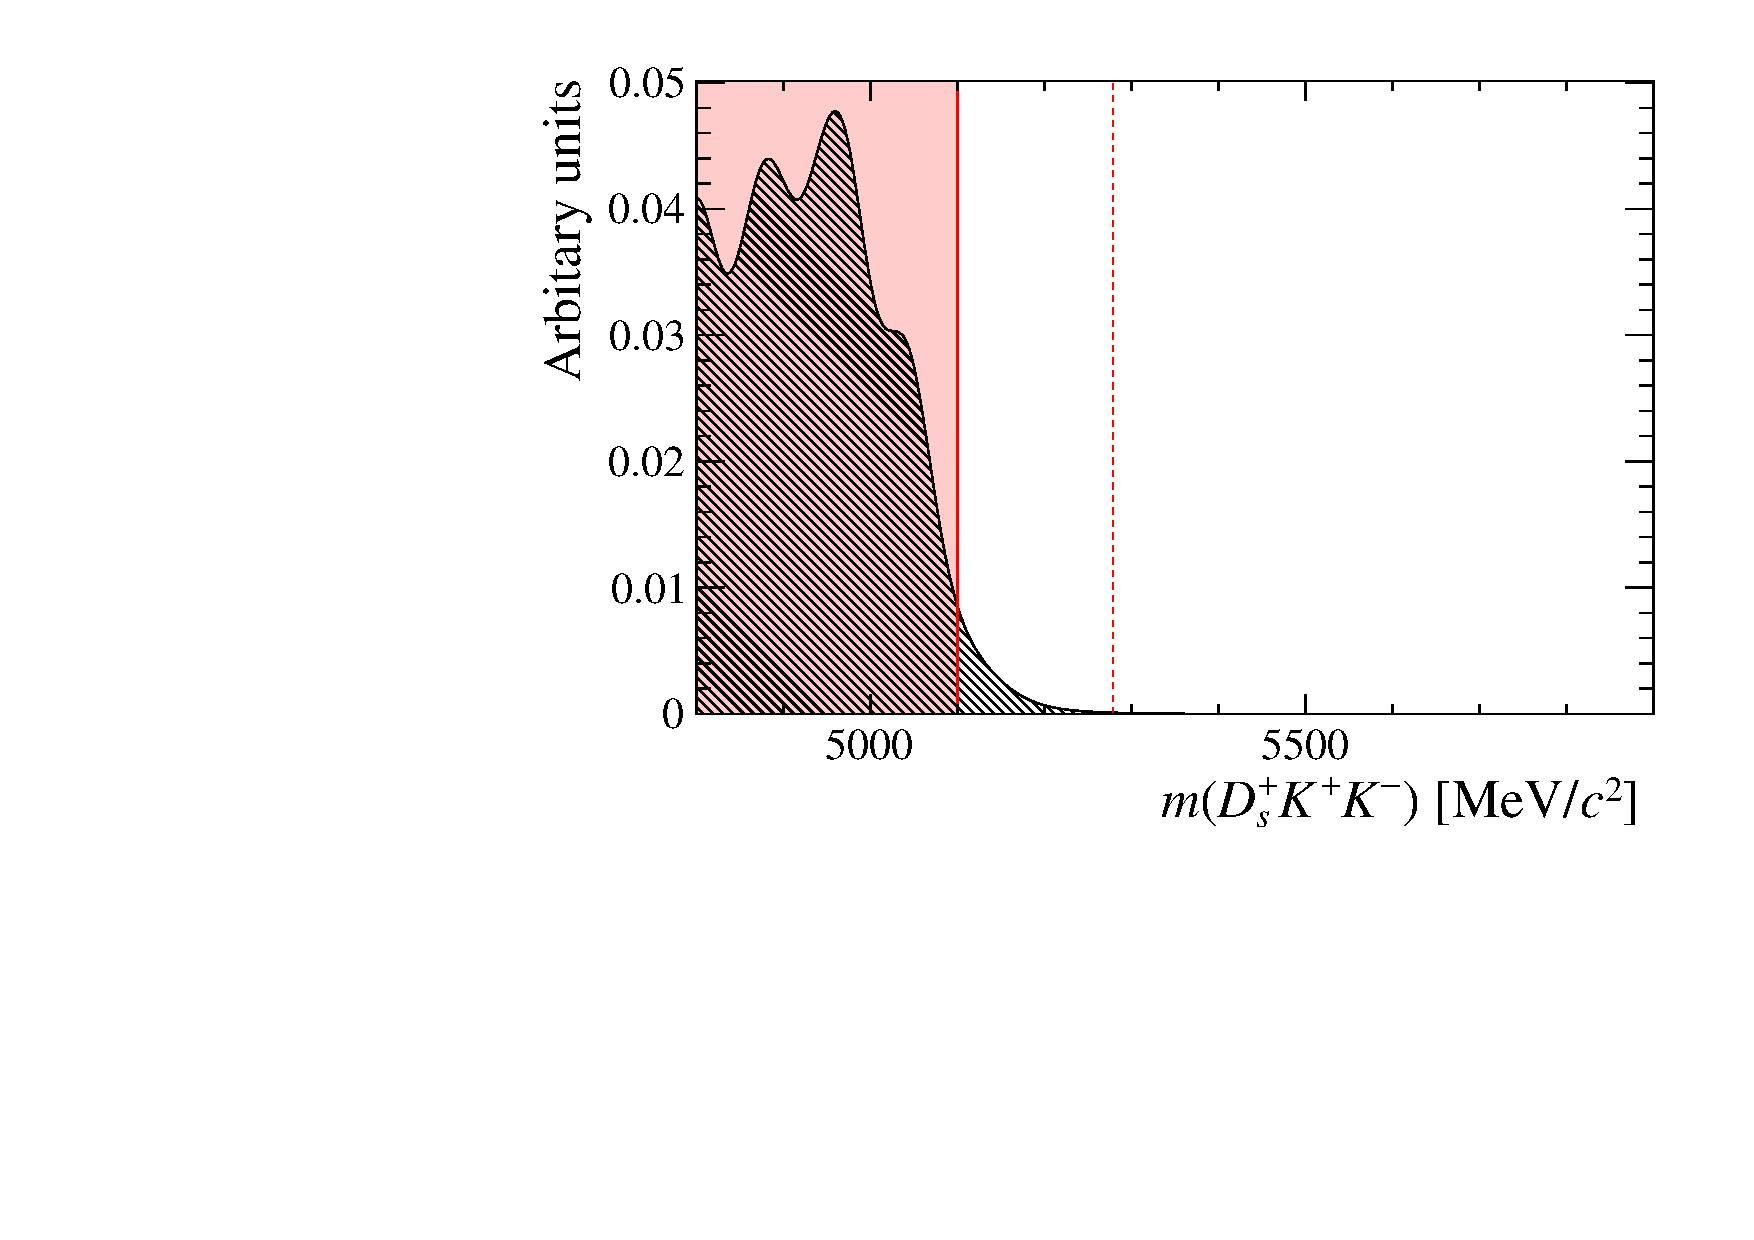
\includegraphics[width=1.0\textwidth]{figs/B2DsKK/Bs2DsstKKst_4800_5900_Shape.pdf}
%         \caption{\decay{\Bsb}{\Dssp\Km\Kstarz}}
%     \end{subfigure}
%     \begin{subfigure}[t]{0.49\textwidth}
%         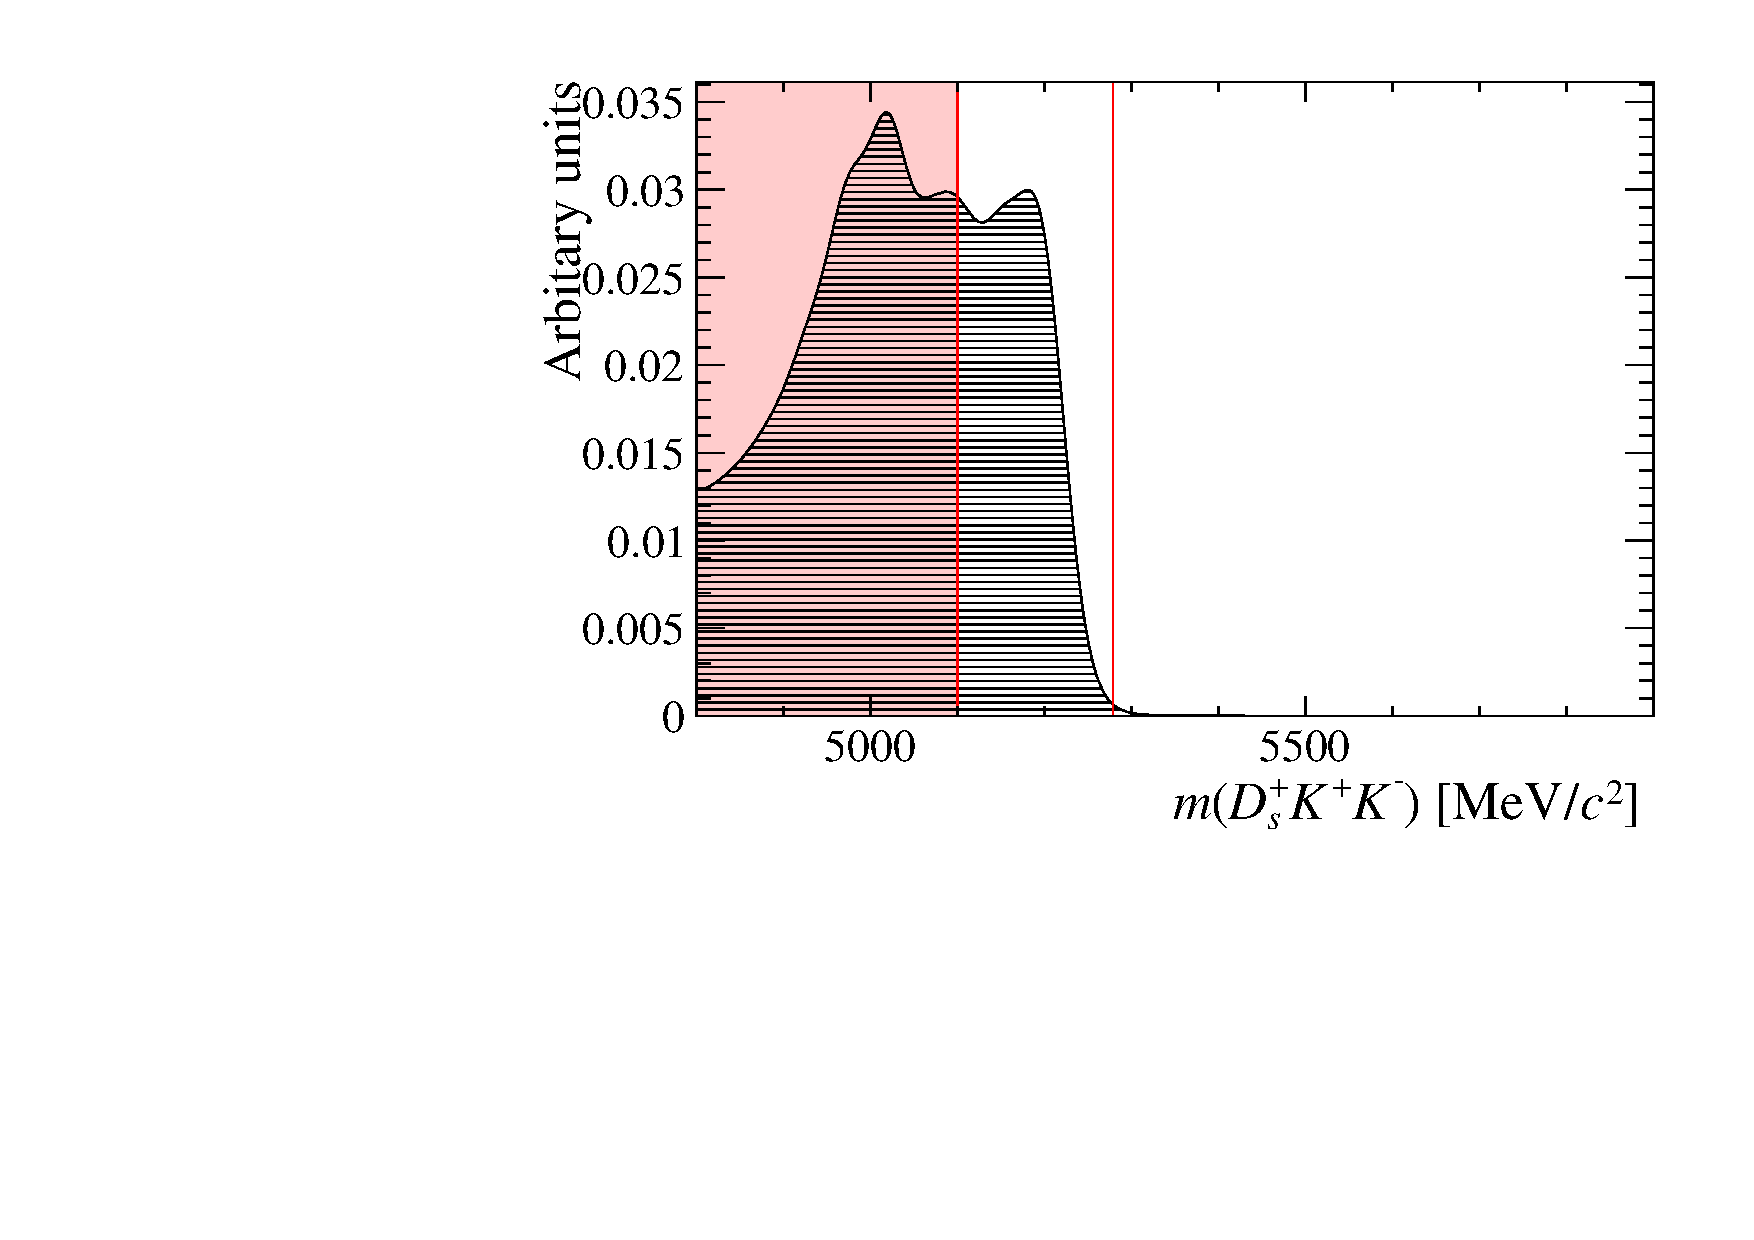
\includegraphics[width=1.0\textwidth]{figs/B2DsKK/Bs2DsDs_4800_5900_Shape.pdf}
%         \caption{\decay{\Bsb}{\Dsp\Dsm} }
%     \end{subfigure}
%     \begin{subfigure}[t]{0.49\textwidth}
%         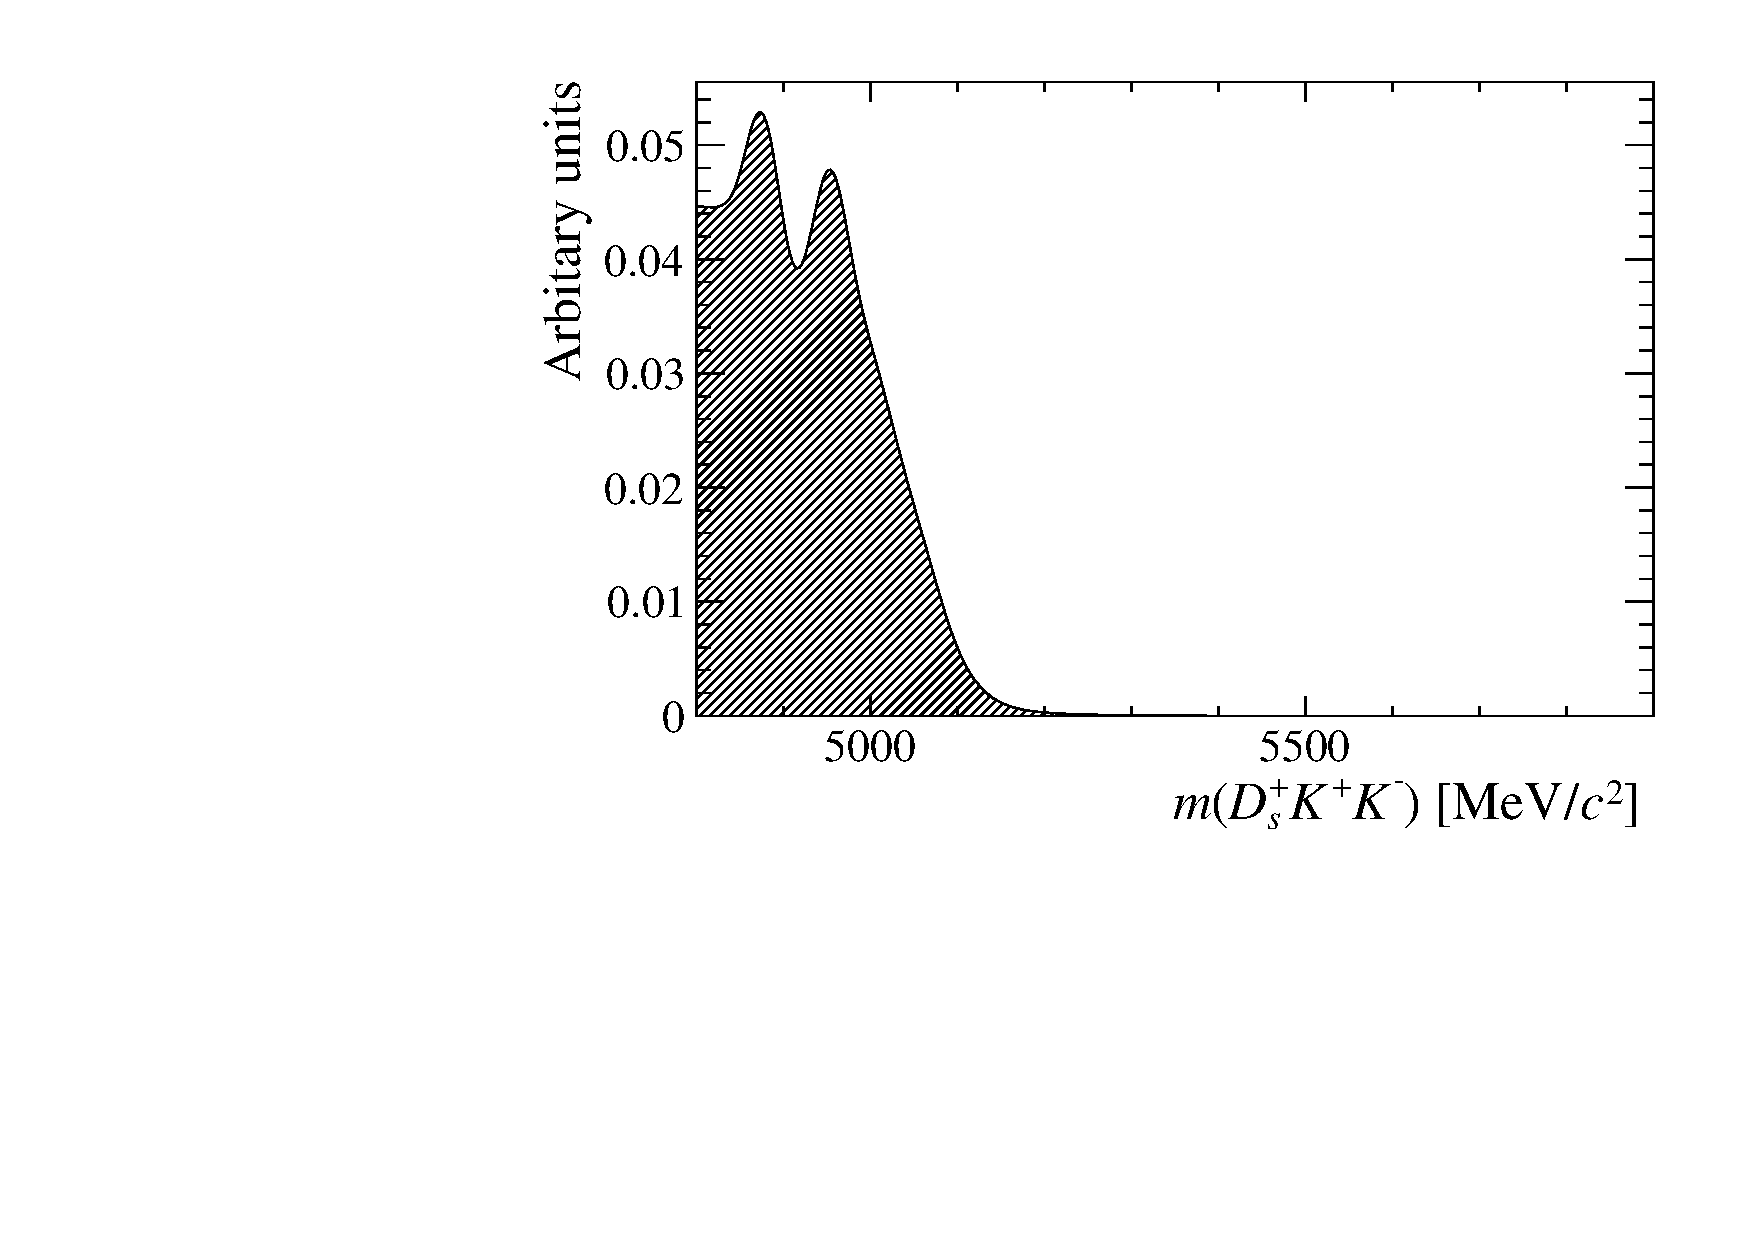
\includegraphics[width=1.0\textwidth]{figs/B2DsKK/Bs2DsstDs_4800_5900_Shape.pdf}
%         \caption{\decay{\Bsb}{\Dssp\Dsm} }
%     \end{subfigure}
%     \caption{Partially reconstructed mass shapes}
%     \label{fig:B2DsKK_part_reco_backgrounds}   
% \end{figure}
% %%%%%%%%%%%%%%%%%%%%%%%%%%%%%%%%%%%%%%%%%%%%%%%%%%%%%%%%%%


\subsection{Combinatorial  background}
\label{sec:B2DsKK_combcomps}

The dominant source of background under the signal peak is due to combinations of unrelated tracks. This combinatorial background is modelled using an exponential function 
\begin{equation}
f(m|c) = e^{-m\times c},
\end{equation}
where $c$ is the single degree of freedom controlling the effective slope of the function and $m$ is the observable \Bp meson invariant mass. The separate fits to the signal and normalisation modes have the freedom to have different combinatorial slopes, motivated by the difference in background levels for the two decays.




\section{Free and constrained parameters}


The fit to signal and normalisation decays have eleven and nine free parameters respectively. These control the yields shapes of the fit components.  
\subsection{Parameter of interest}
\begin{description}
\item \textbf{Signal:} the parameter of interest in the signal decay is $N(\decay{\Bp}{\Dsp\Kp\Km})$, the yield attributed to the signal PDF.

\item \textbf{Normalisation:} the parameter of interest in the signal decay is $N(\decay{\Bp}{\Dsp\Dzb})$, the yield attributed to the normalisation PDF. 

\end{description}

          %         nsig    4.4287e+02    4.4277e+02 +/-  2.94e+01  <none>
          %         nsig    1.0905e+03    1.0905e+03 +/-  3.42e+01  <none>

\subsection{Shape parameters}
\begin{description}
\item \textbf{Signal:} The signal fit contains four free parameters that determine the shape of various PDFs. This corresponds to the mass offset $\delta$, signal mean value $\mu$, signal width $\sigma_{1}$ and combinatorial slope $c$.
          % global_shift    2.2538e+00    3.5457e+00 +/-  1.17e+01  <none>
          %       mean_B    5.2789e+03    5.2789e+03 +/-  8.82e-01  <none>
          %        sigma    1.2298e+01    1.2291e+01 +/-  8.77e-01  <none>
          %        slope   -2.8199e-03   -2.8202e-03 +/-  2.79e-04  <none>
\item \textbf{Normalisation:} The normalisation fit has five free parameters that control the distributions of the signal and background PDFs. This includes the mean \Bp mass $\mu$, signal width $\sigma_{1}$, the combinational slope $c$, the mass offset $\delta$ and the relative heights of the double peaked partially reconstructed shapes $\xi$.   
          %   global_csi    1.2683e-06    5.2233e-08 +/-  2.25e-01  <none>
          % global_shift   -1.0585e+01   -1.0586e+01 +/-  1.31e+00  <none>
          %       mean_B    5.2784e+03    5.2784e+03 +/-  4.00e-01  <none>
          %        slope   -9.4305e-03   -9.4308e-03 +/-  1.13e-03  <none>
          %        sigma    1.2436e+01    1.2435e+01 +/-  3.23e-01  <none>
\end{description}

\subsection{Yields}
\begin{description}
\item \textbf{Signal:} the yields of each background component are left free in the signal fit. This corresponds to six free parameters for $N_{\text{comb}}$, $N(\decay{\Bsb}{\Dsp\Km\Kstarz})$, $N(\decay{\Bsb}{\Dssp\Km\Kstarz})$, $N(\decay{\Bs}{\Dsp\Dsm})$, $N(\decay{\Bz}{\Dsp\Dm})$, and $N(\decay{\Bs}{\Dssp\Dsm})$.

          %          nBG    1.1139e+03    1.1142e+03 +/-  7.30e+01  <none>
          %     nBs2Dsa1    1.1153e+03    1.1147e+03 +/-  4.61e+02  <none>
          % nBs2DsstKKst    2.9756e+02    2.9691e+02 +/-  1.24e+02  <none>
          %     nBs2DsDs    2.0262e+02    2.0307e+02 +/-  5.08e+02  <none>
          %      nB02DsD    4.6587e+02    4.6621e+02 +/-  1.54e+02  <none>
          %   nBs2DsstDs    1.1208e-04    6.2385e-02 +/-  3.98e+02  <none>
\item \textbf{Normalisation:} the yields of the combinatorial and partially reconstructed backgrounds are left free in the fit to the normalisation channel. This corresponds to three parameters; $N_{\text{comb}}$, $N(\decay{\Bp}{\Dssp\Dzb})$ and $N(\decay{\Bp}{\Dsp\Dstarzb})$. The relatives contributions of the \decay{\Dssp}{\Dsp\piz} and \decay{\Dssp}{\Dsp\Pgamma} decays are fixed to their ratio of branching fractions (similarly for \Dstarzb). A factor is included to account for the fraction of each PDF that is within the fitted \Bp invariant mass range.
\end{description}

          %          nBG    2.4773e+02    2.4769e+02 +/-  5.42e+01  <none>
          %      nDsDst0    3.3055e+02    3.3055e+02 +/-  6.72e+01  <none>
          %      nDsstD0    7.5230e+02    7.5220e+02 +/-  5.48e+01  <none>



\section{Fit validation}
\label{sec:B2DsKK_fitvalidation}

The fitting framework is validated using large quantities of pseudo-experiments randomly generated using the same fit model. The free parameters are treated using the plug-in method~\cite{plugin}; the generated values of all free parameters are \emph{plugged in} using the fitted values from the fit to data.      

The fitted values and uncertainties are determined for each pseudo-experiment and a corresponding pull determined, defined as
\begin{equation}
g_{\text{pull}} = \frac{x_{\text{fit}} - x_{\text{gen}} }{\sigma}
\end{equation}
where $x_{\text{gen}}$ and $x_{\text{fit}}$ are the generated and fitted values of the variable, and $\sigma$ is the parameter's uncertainty.
For an ideal unbiased fit model, the pull of each parameter of interest would be normally distributed with unit width and mean of zero.  


%%%%%%%%%%%%%%%%%%%%%%%%%%%%%%%%%%%%%%%%%%%%%%%%%%%%%%%%%%
\begin{figure}[!h]
   \centering
   \begin{subfigure}[t]{1.0\textwidth}
      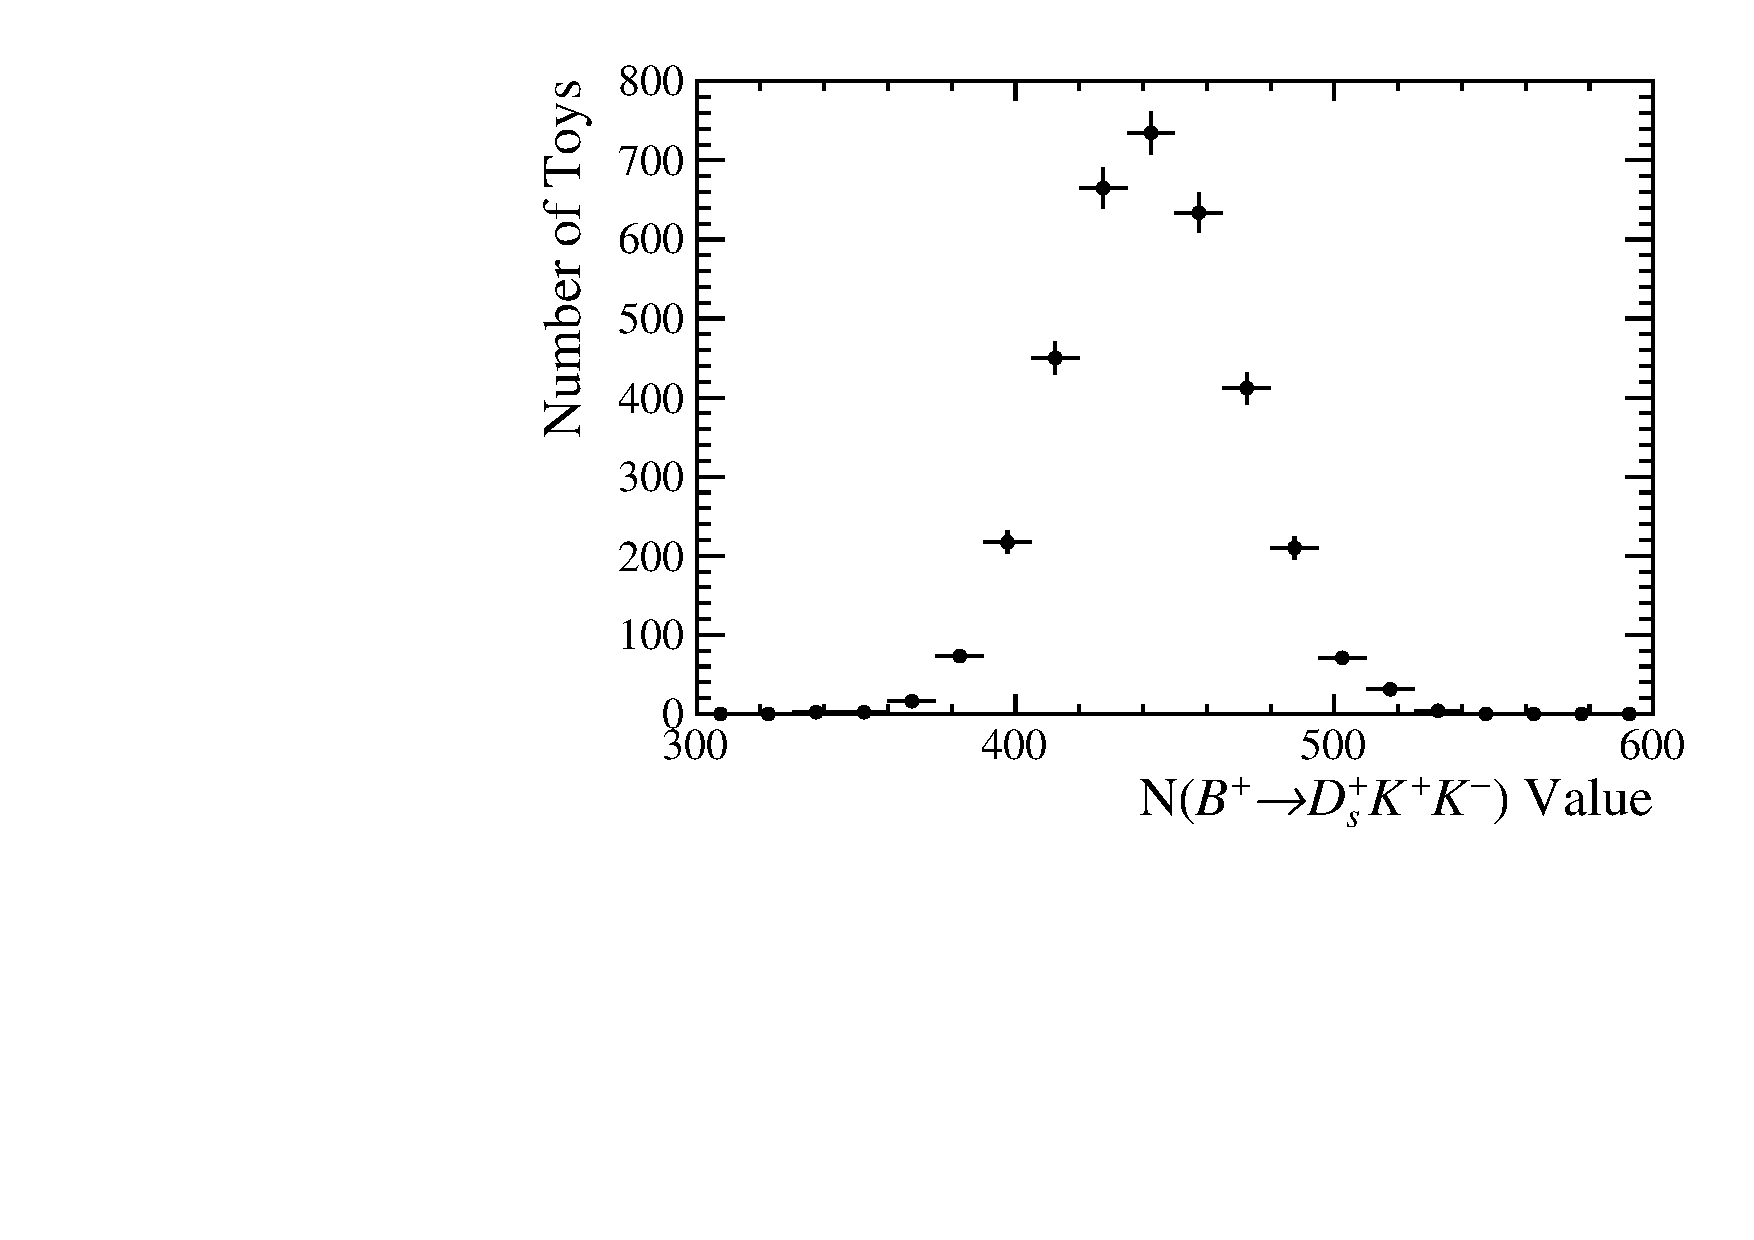
\includegraphics[width=0.32\textwidth]{figs/B2DsKK/Plots_DsKK_nsig_val.pdf}
      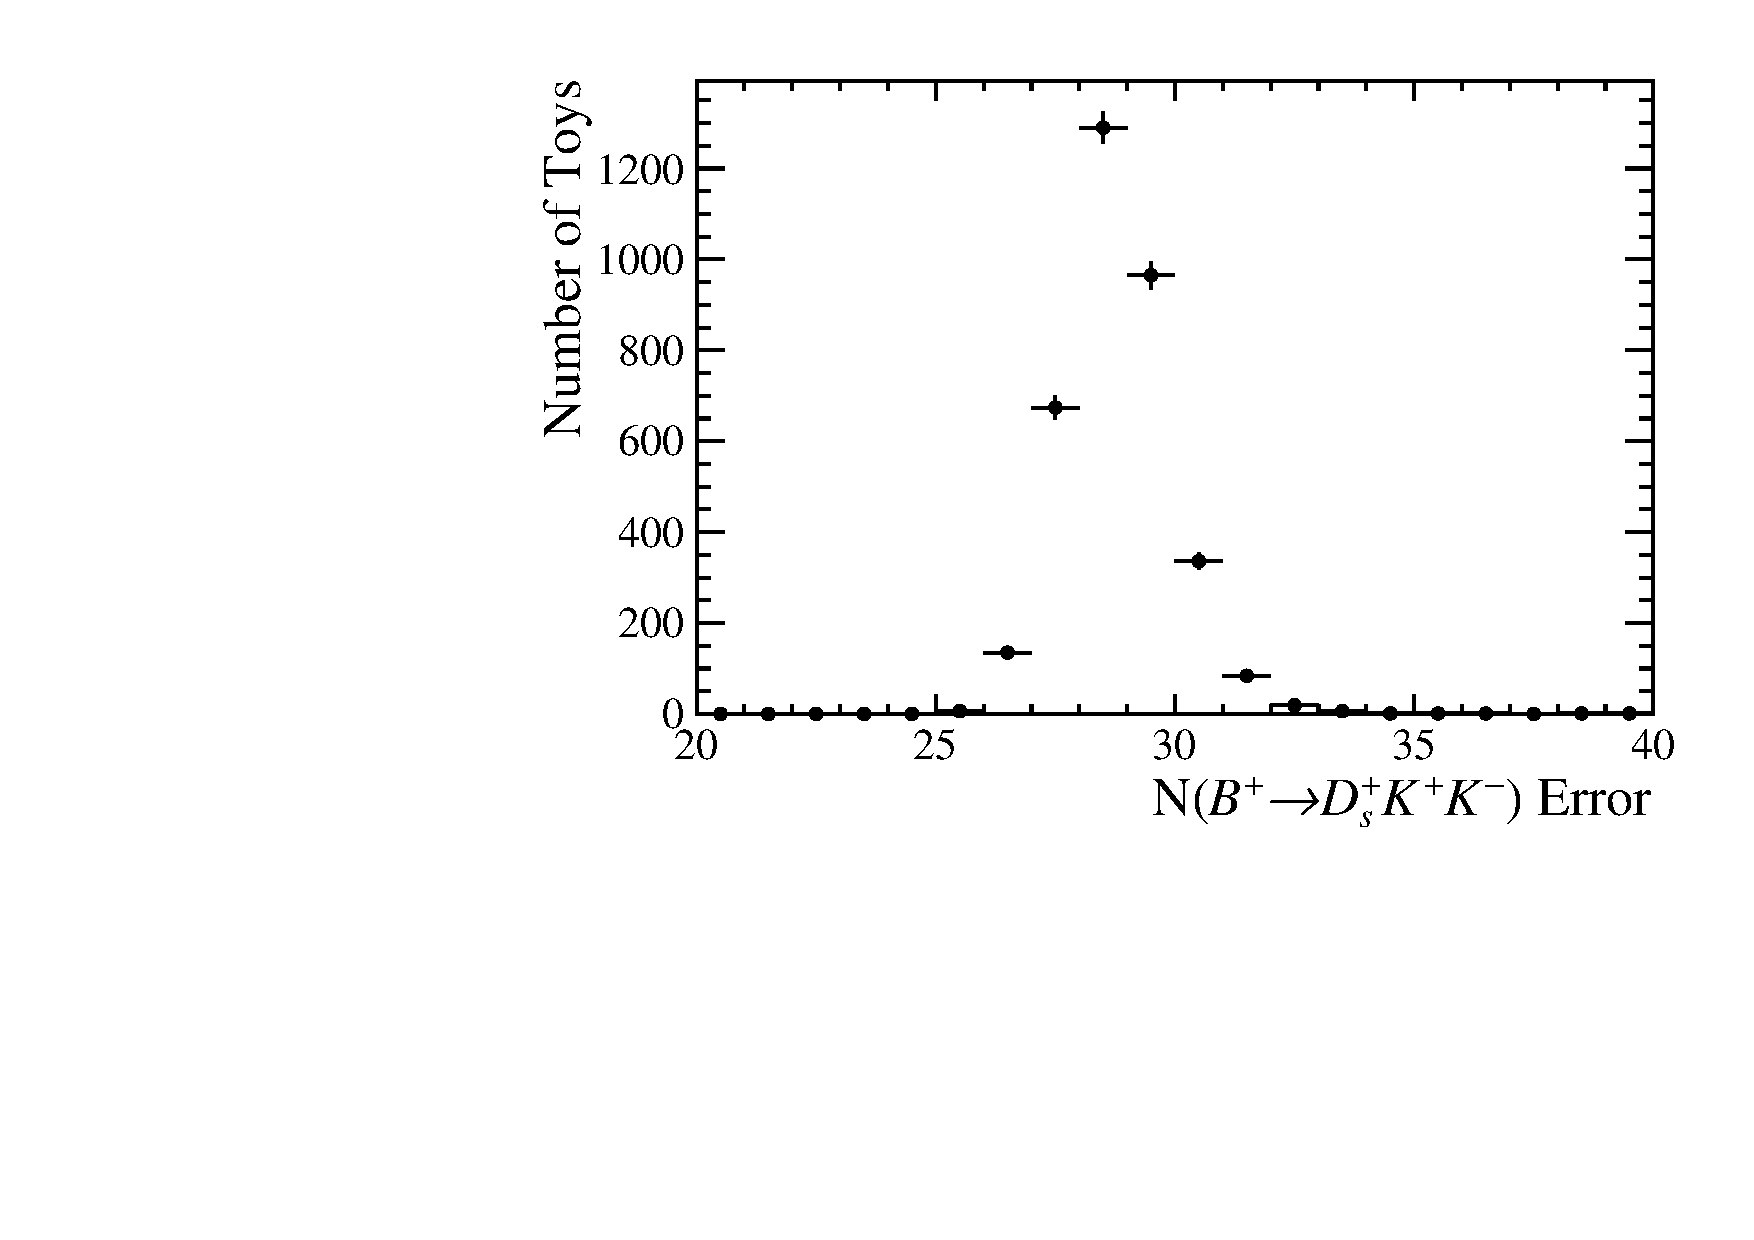
\includegraphics[width=0.32\textwidth]{figs/B2DsKK/Plots_DsKK_nsig_err.pdf}
      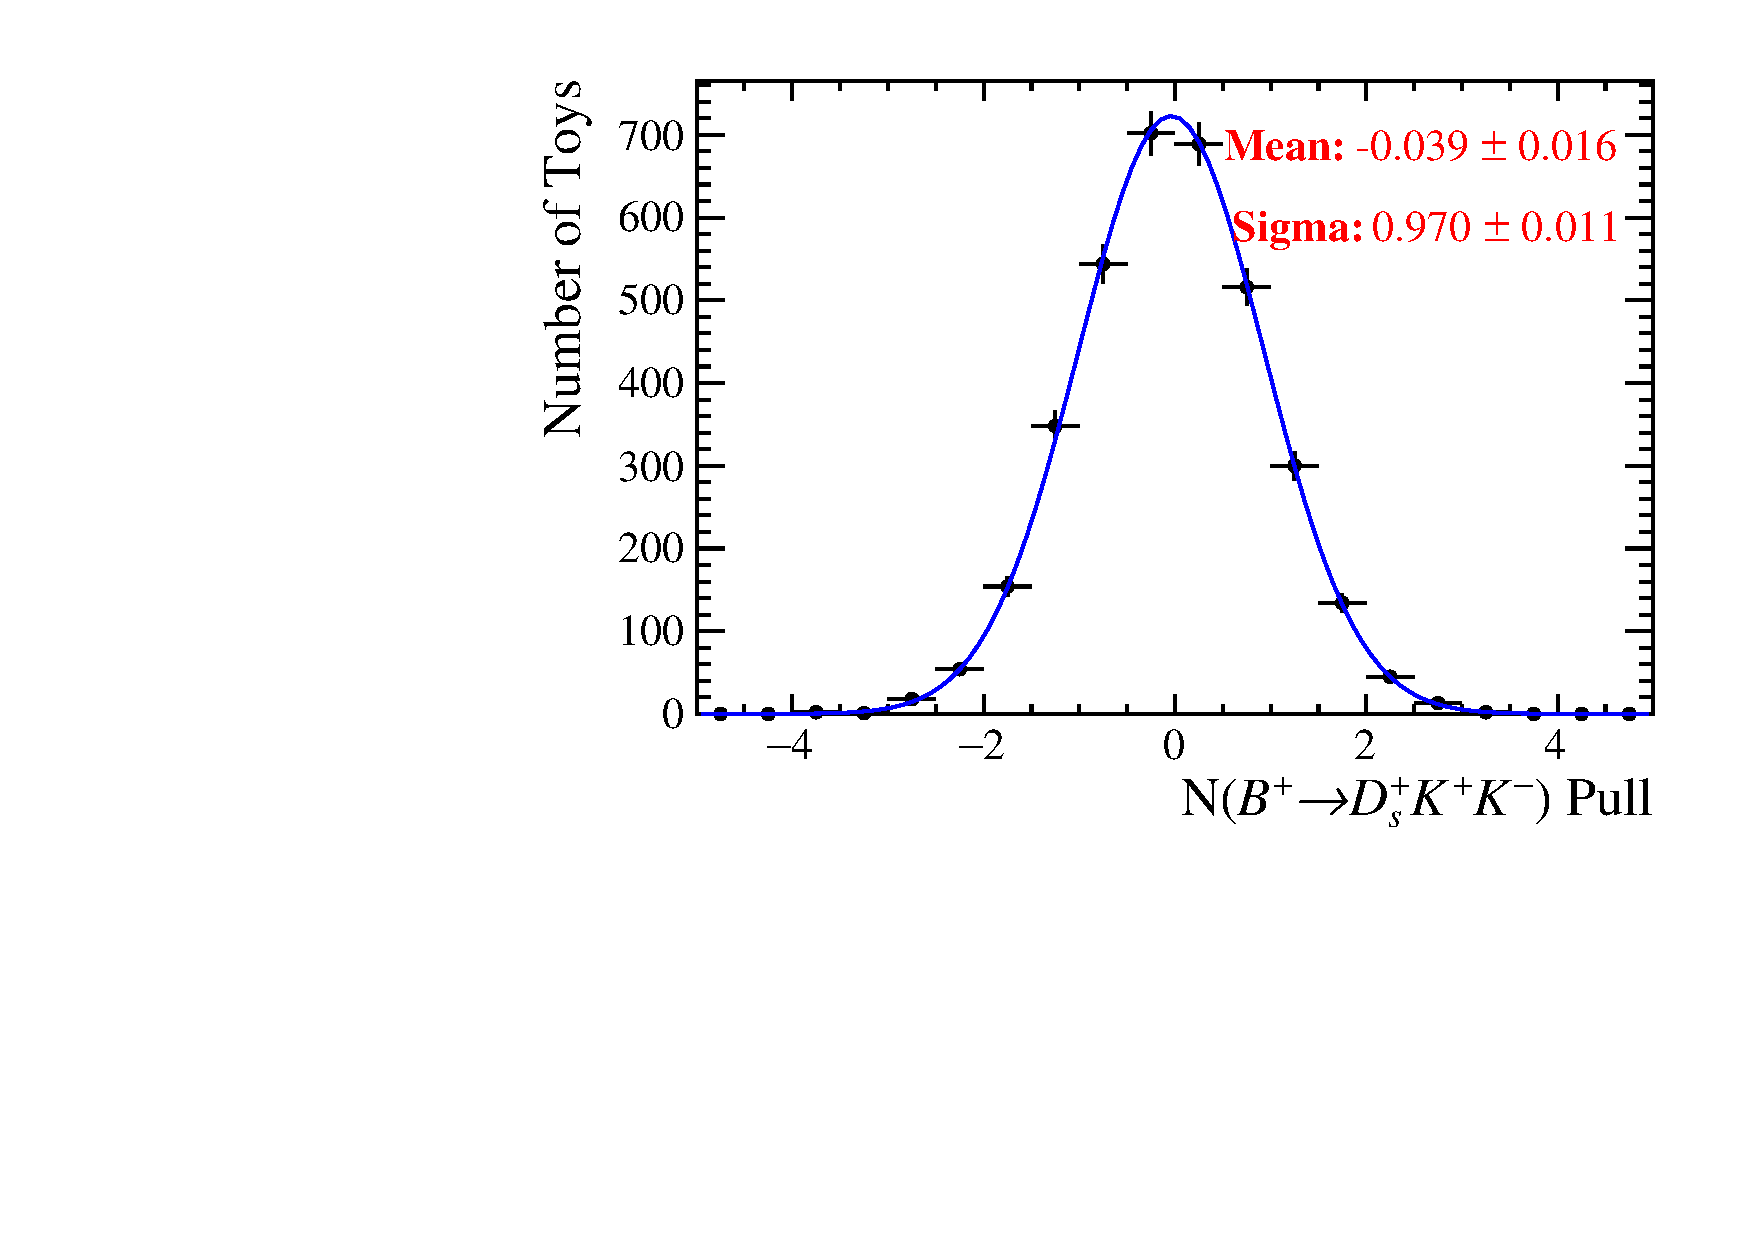
\includegraphics[width=0.32\textwidth]{figs/B2DsKK/Plots_DsKK_nsig_pul.pdf}
      \caption{Signal fit}
   \end{subfigure}\\
   \begin{subfigure}[t]{1.0\textwidth}
      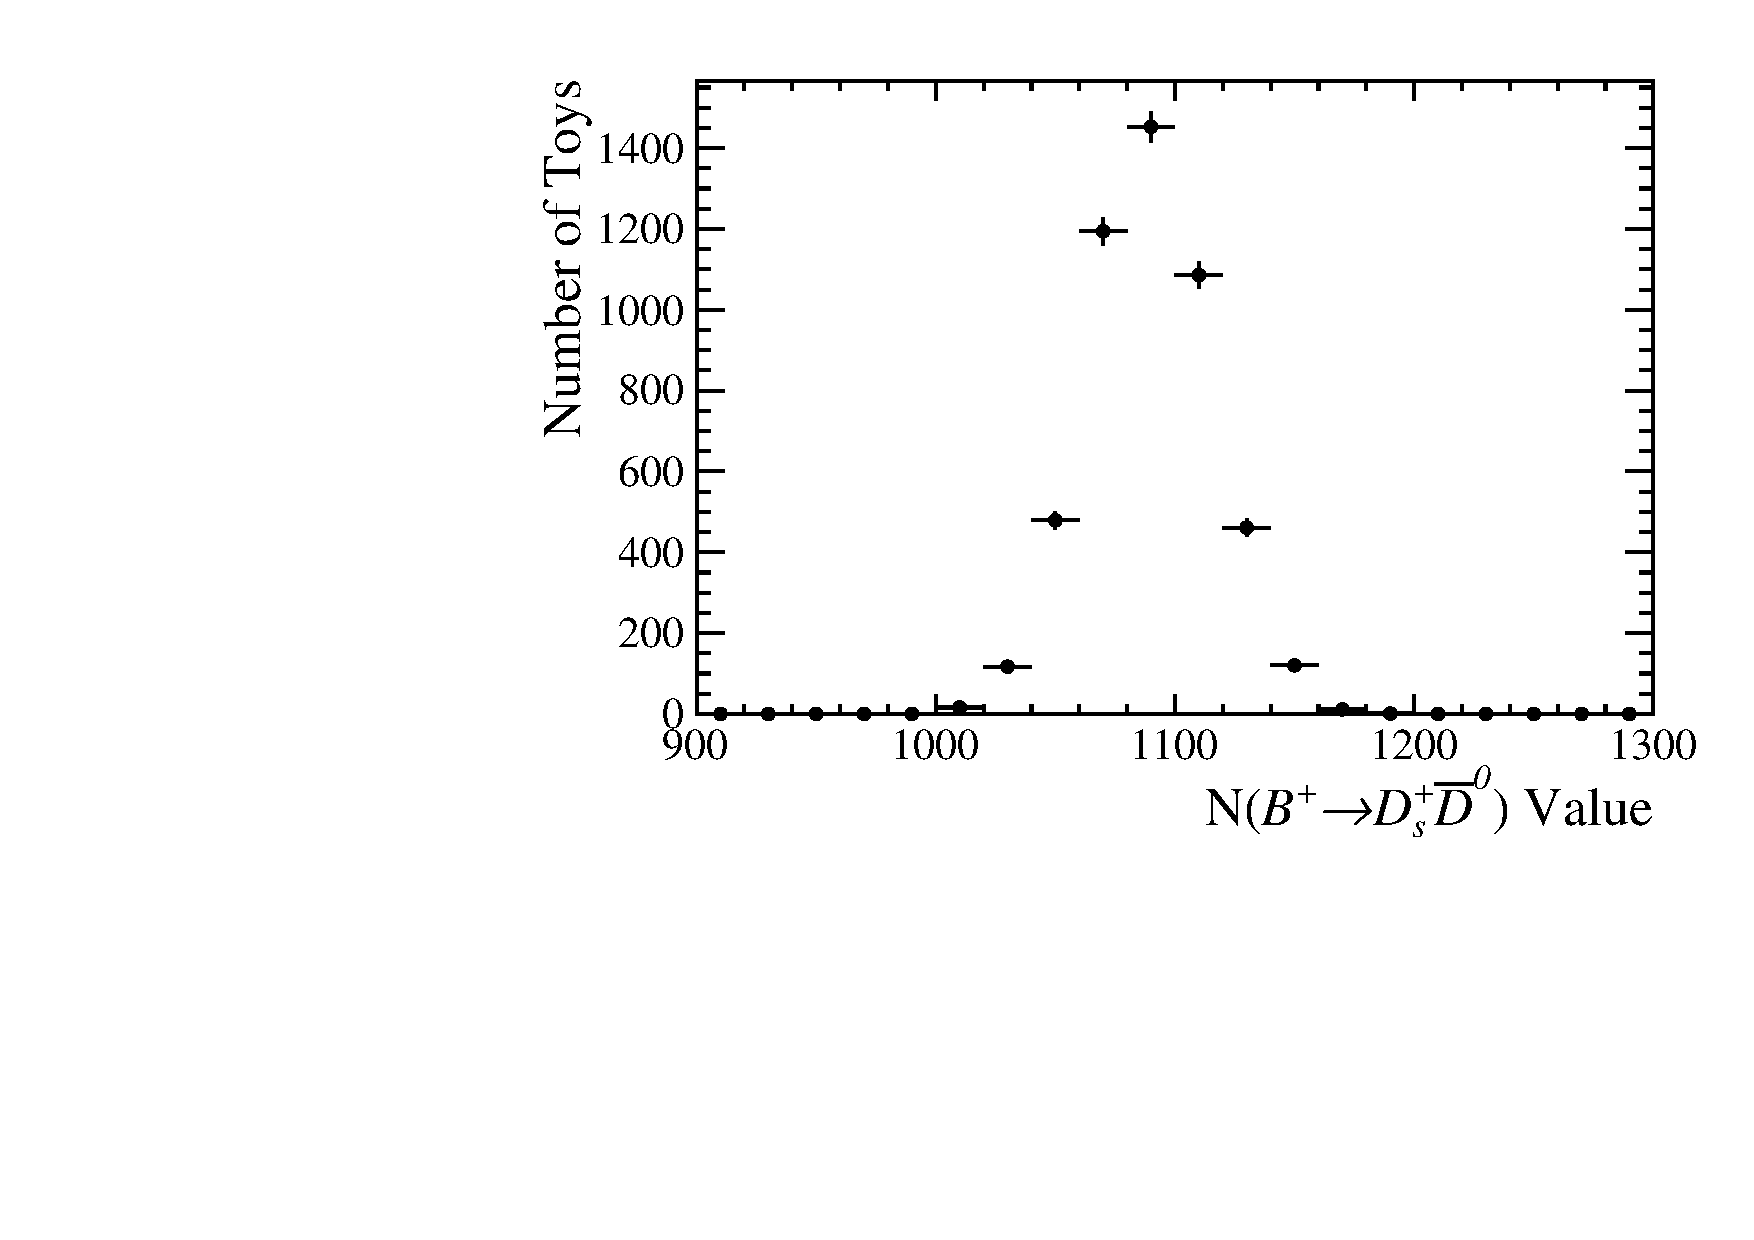
\includegraphics[width=0.32\textwidth]{figs/B2DsKK/Plots_DsD0_nsig_val.pdf}
      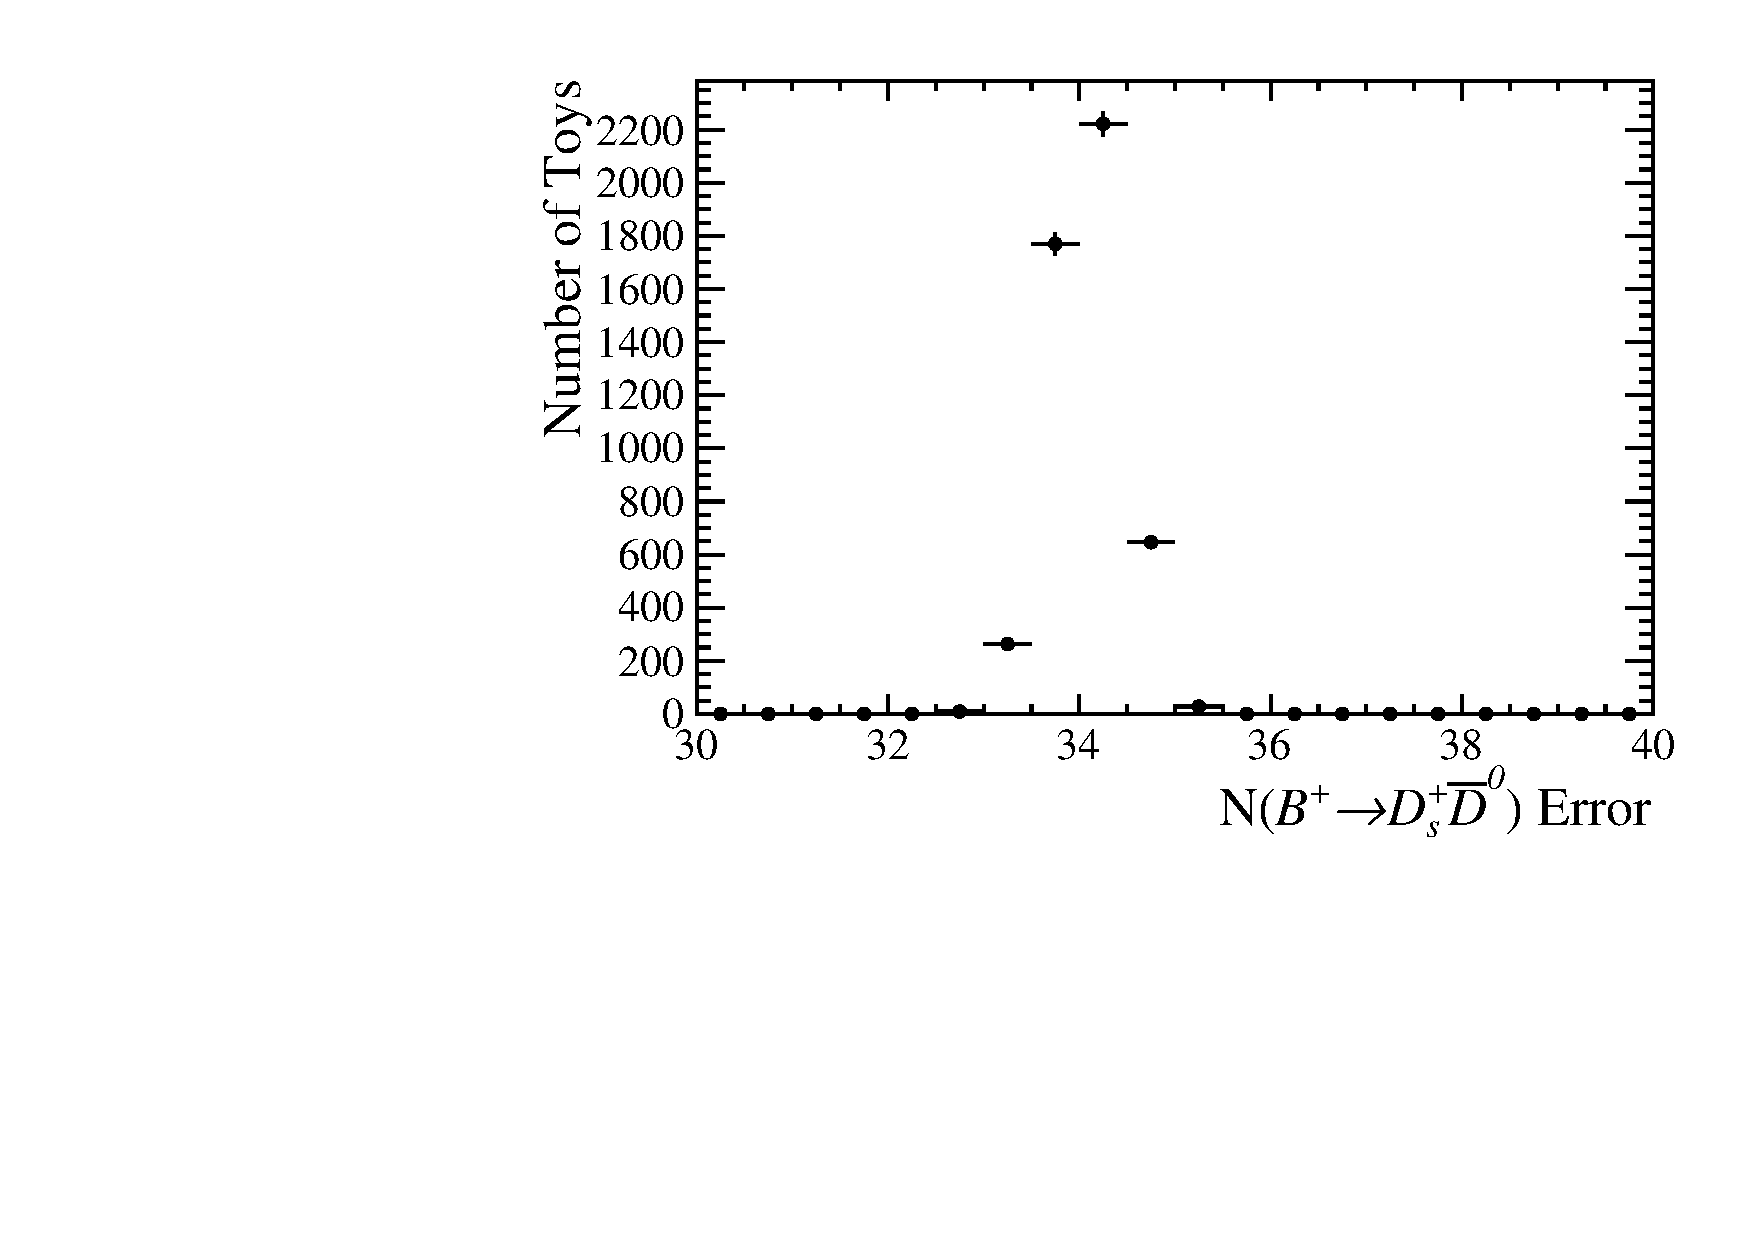
\includegraphics[width=0.32\textwidth]{figs/B2DsKK/Plots_DsD0_nsig_err.pdf}
      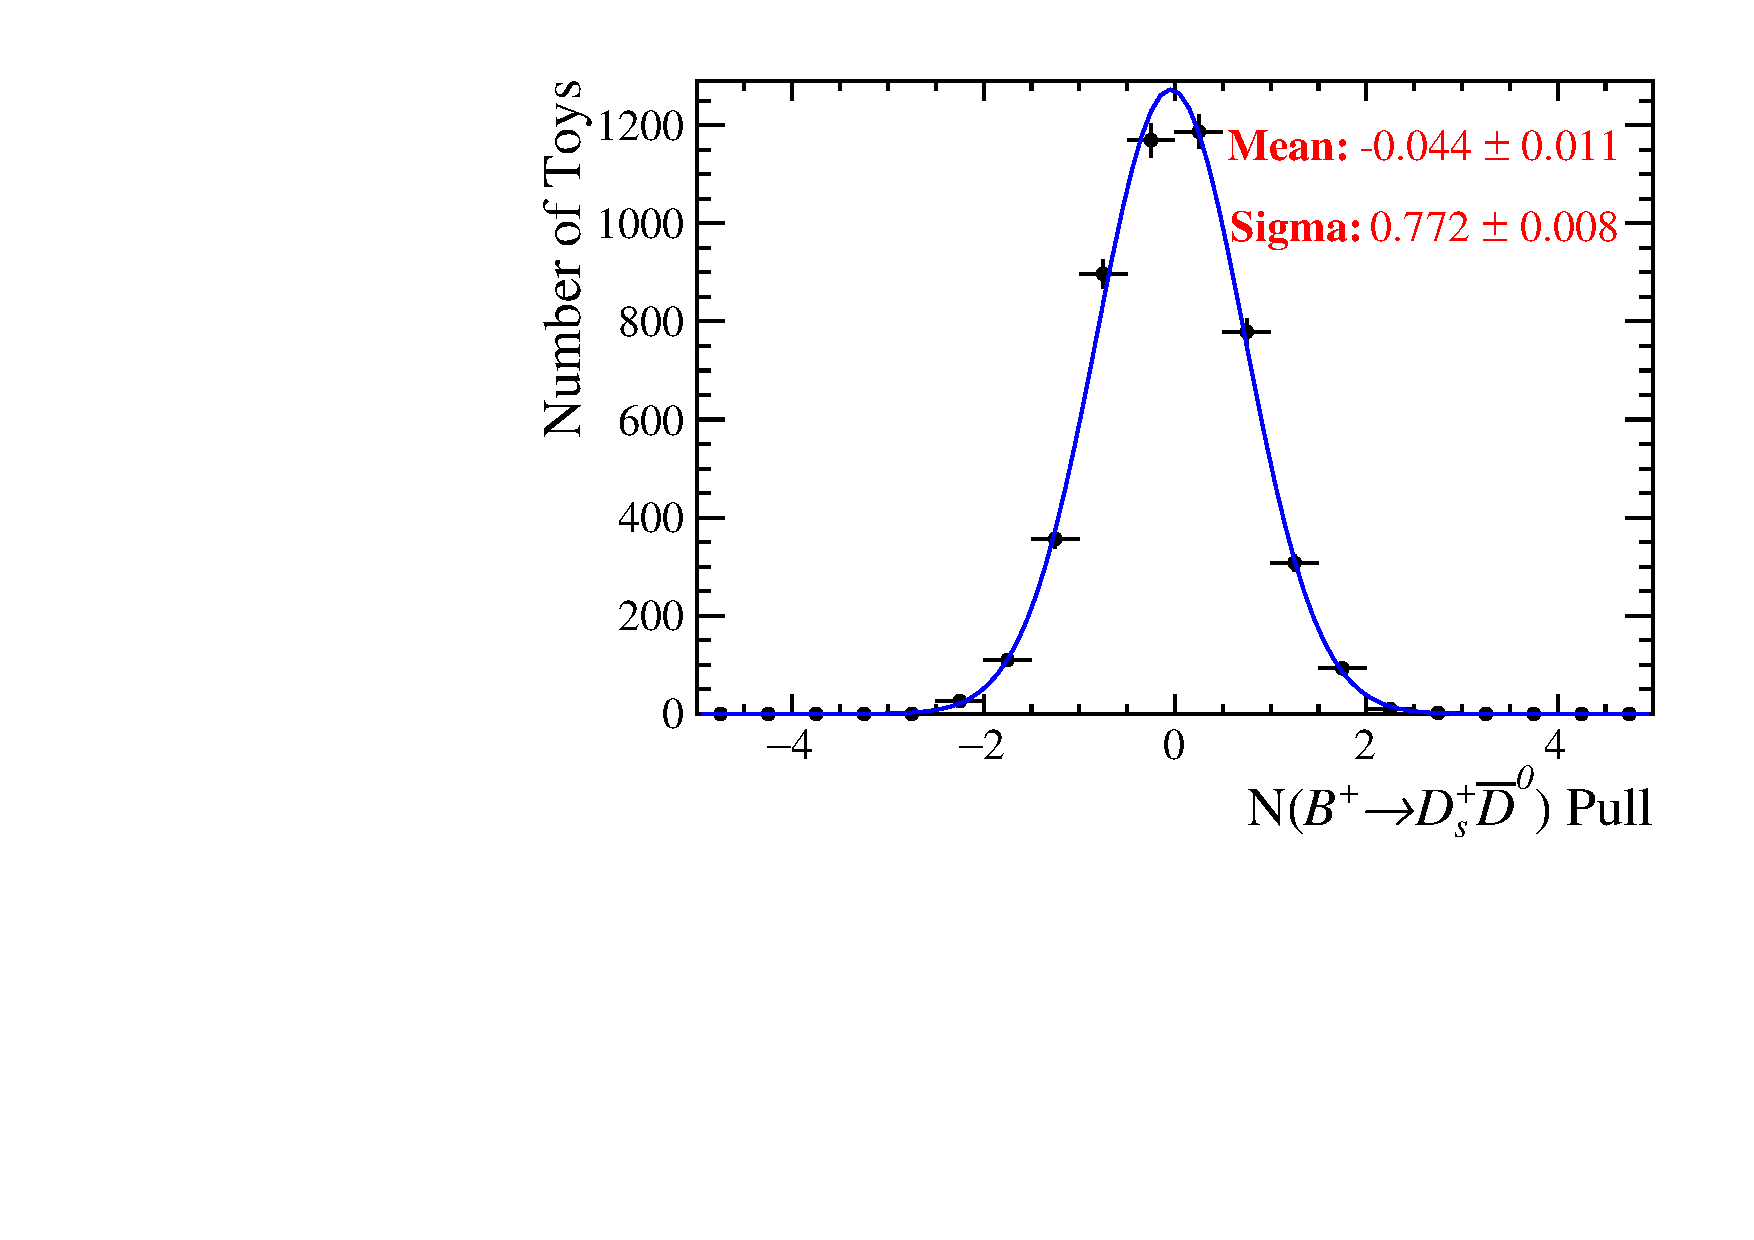
\includegraphics[width=0.32\textwidth]{figs/B2DsKK/Plots_DsD0_nsig_pul.pdf}
      \caption{Normalisation fit}
   \end{subfigure}\\
   \caption{The distribution of the signal and normalisation yields, errors and pulls as determined from pseudo-experiments. The result of fit performed to the pull distributions is overlaid in blue, along with the numerical results in red.}
   \label{fig:B2DsKK_Pulls}
\end{figure}
%%%%%%%%%%%%%%%%%%%%%%%%%%%%%%%%%%%%%%%%%%%%%%%%%%%%%%%%%%

The distributions of the yields, errors and pulls for the signal and normalisation pseudo-experiments are shown in Fig.~\ref{fig:B2DsKK_Pulls}. A fit is performed for each pull distributions using a Gaussian to determine the mean and width. 
For the signal yield the mean and with are within $3\sigma$ of zero and one respectively. The normalisation yield shows a significant bias in the width. The bias implies the fit model is overestimating the uncertainty $\sigma$ of the yield.
If the normalisation yield uncertainty dominates the uncertainty in the branching fraction this could lead to an overestimation of the uncertainty on the final measured branching fraction.

To determine how the normalisation uncertainty propagates to the branching fraction another set of pseudo-experiments are produced.
This set includes both signal and normalisation decays. To calculated the branching fraction the yield of \decay{\Bp}{\Dsp\Kp\Km} decays is corrected according to the signal efficiency as a function of the kinematics of a given candidate, as detailed previously in Eq.~\ref{eq:B2DsKK_corrected_yield}. The candidates are assumed to have a flat distribution in the two dimensional $m^{2}(\Kp\Km)$ vs. $m^{2}(\Dsp\Km)$ space used to parametrise the efficiency. For each pseudo-experiment the branching fraction and uncertainty are produced. As no branching fraction is explicitly used to generate the pseudo-experiment (rather independent signal and normalisation yields), the pulls are redefined to be measured relative to the mean branching fraction
\begin{equation}
g_{\text{pull}} = \frac{x_{\text{fit}} - \bar{x}_{\text{fit}} }{\sigma}
\end{equation}
where $x_{\text{fit}}$ is the fitted value of the parameter, $\bar{x}_{\text{fit}}$ is the average of all fitted values and $\sigma$ is the uncertainty. The distribution of the branching fraction, uncertainty and pull are shown in Fig~\ref{fig:B2DsKK_BR_Pulls}. 


%%%%%%%%%%%%%%%%%%%%%%%%%%%%%%%%%%%%%%%%%%%%%%%%%%%%%%%%%%
\begin{figure}[!h]
   \centering
   \begin{subfigure}[t]{1.0\textwidth}
      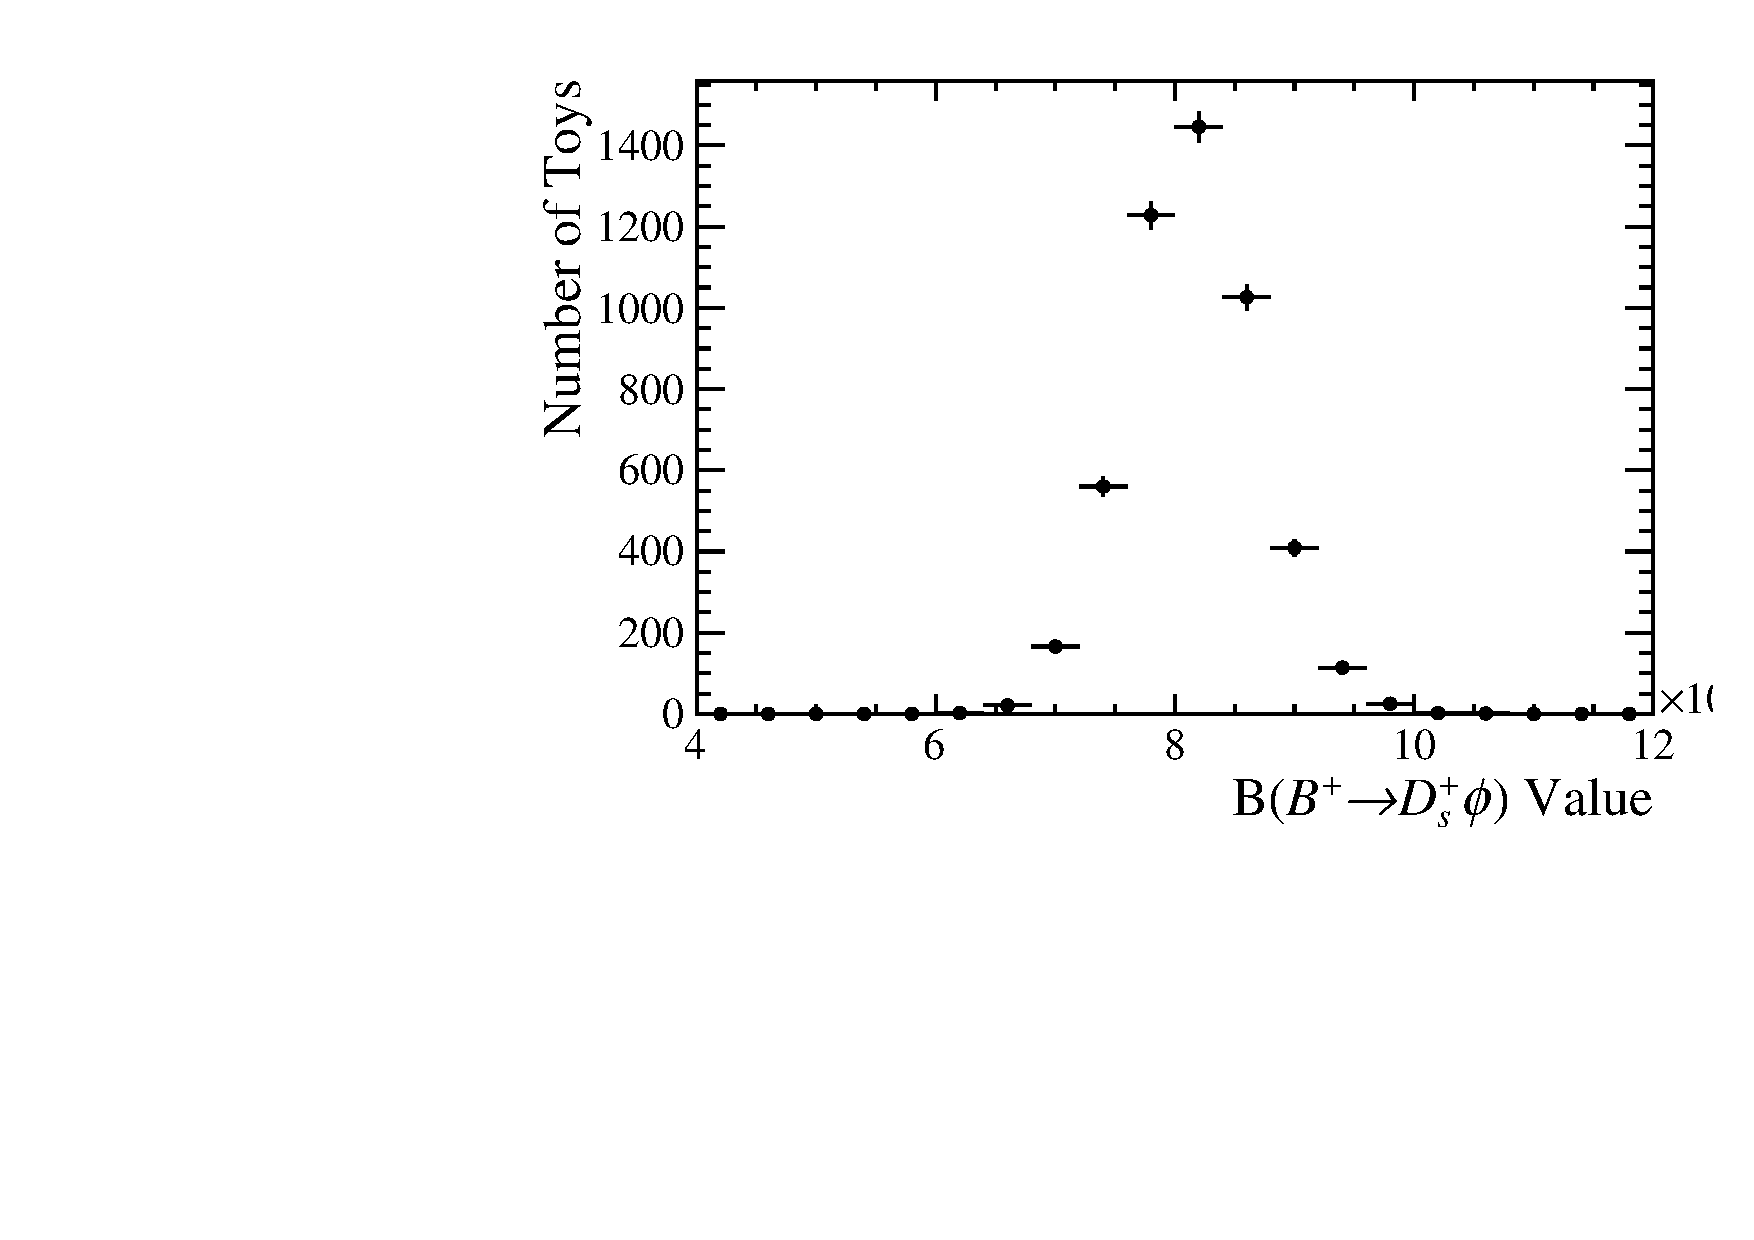
\includegraphics[width=0.32\textwidth]{figs/B2DsKK/Branching_Fraction_val.pdf}
      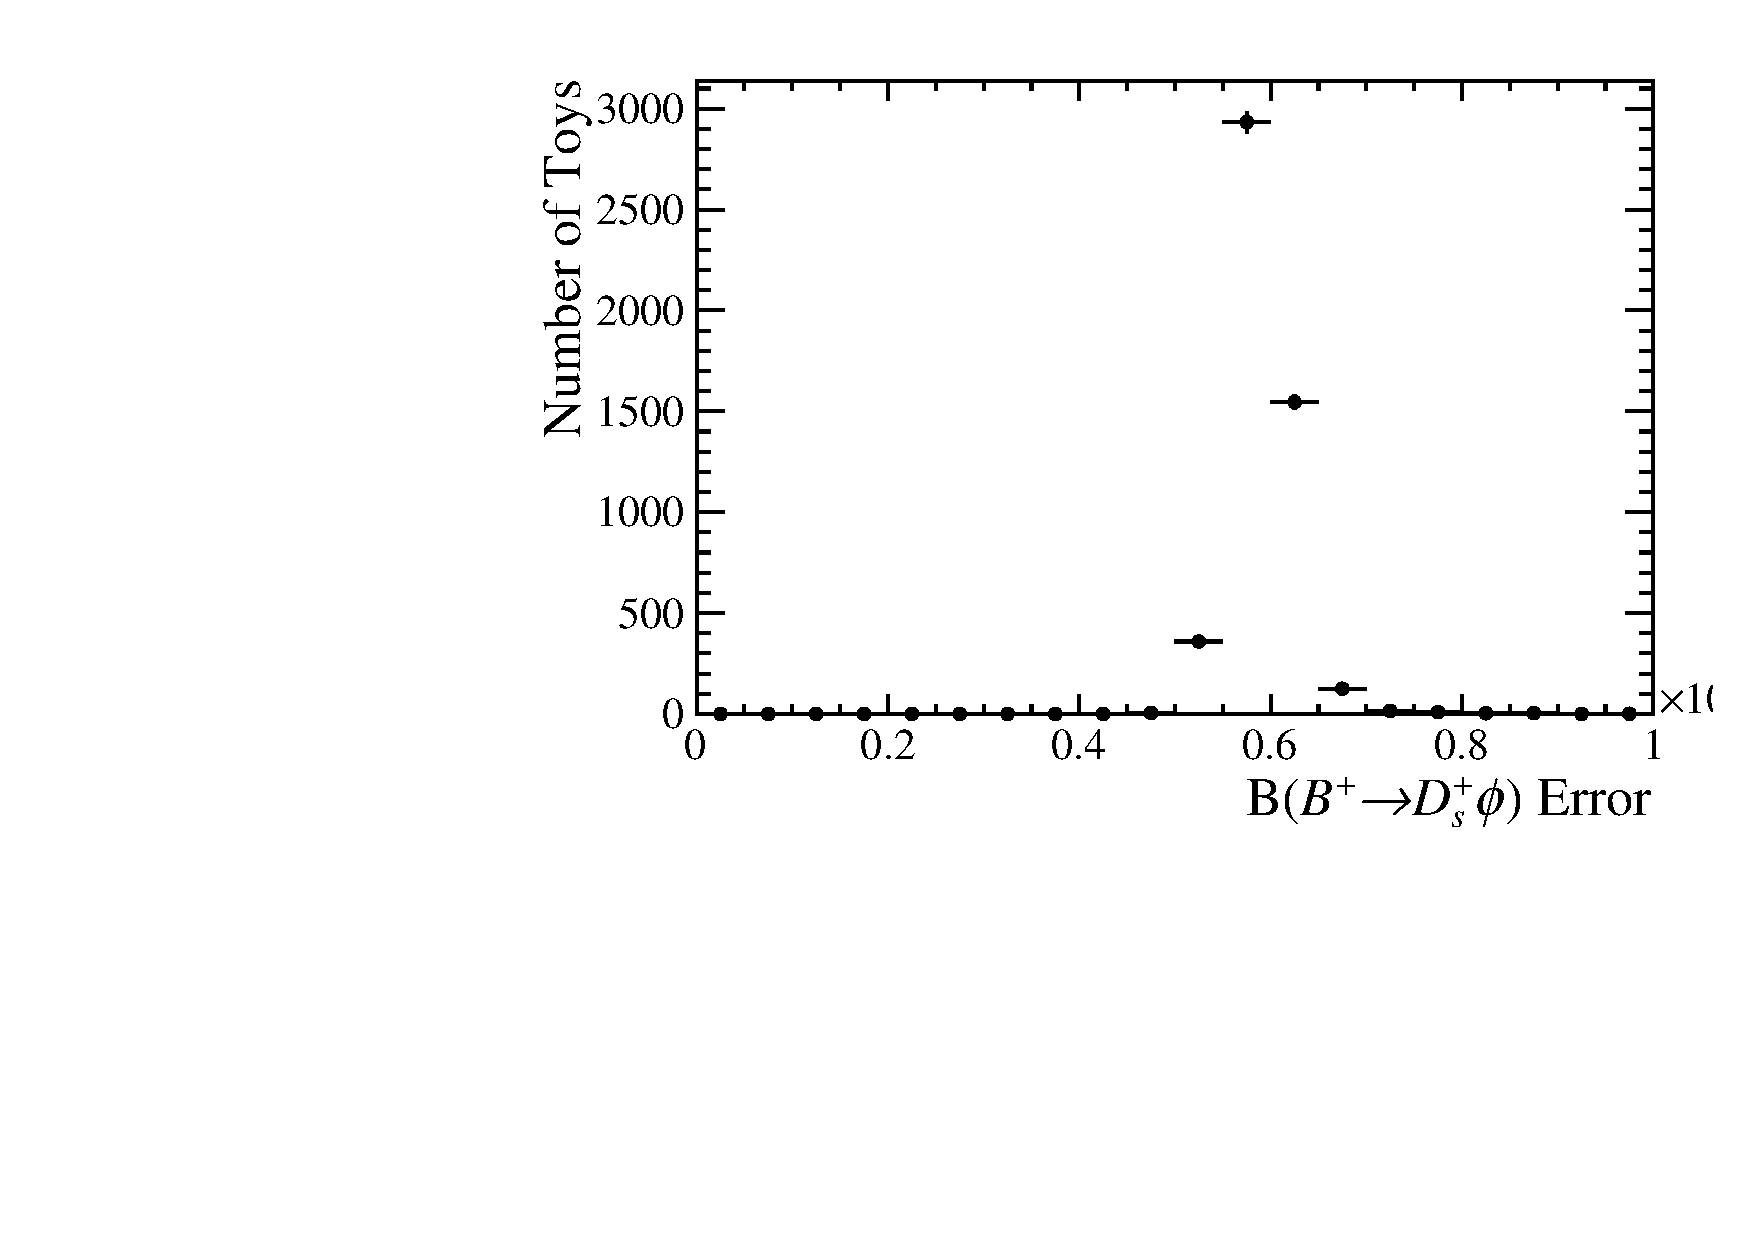
\includegraphics[width=0.32\textwidth]{figs/B2DsKK/Branching_Fraction_err.pdf}
      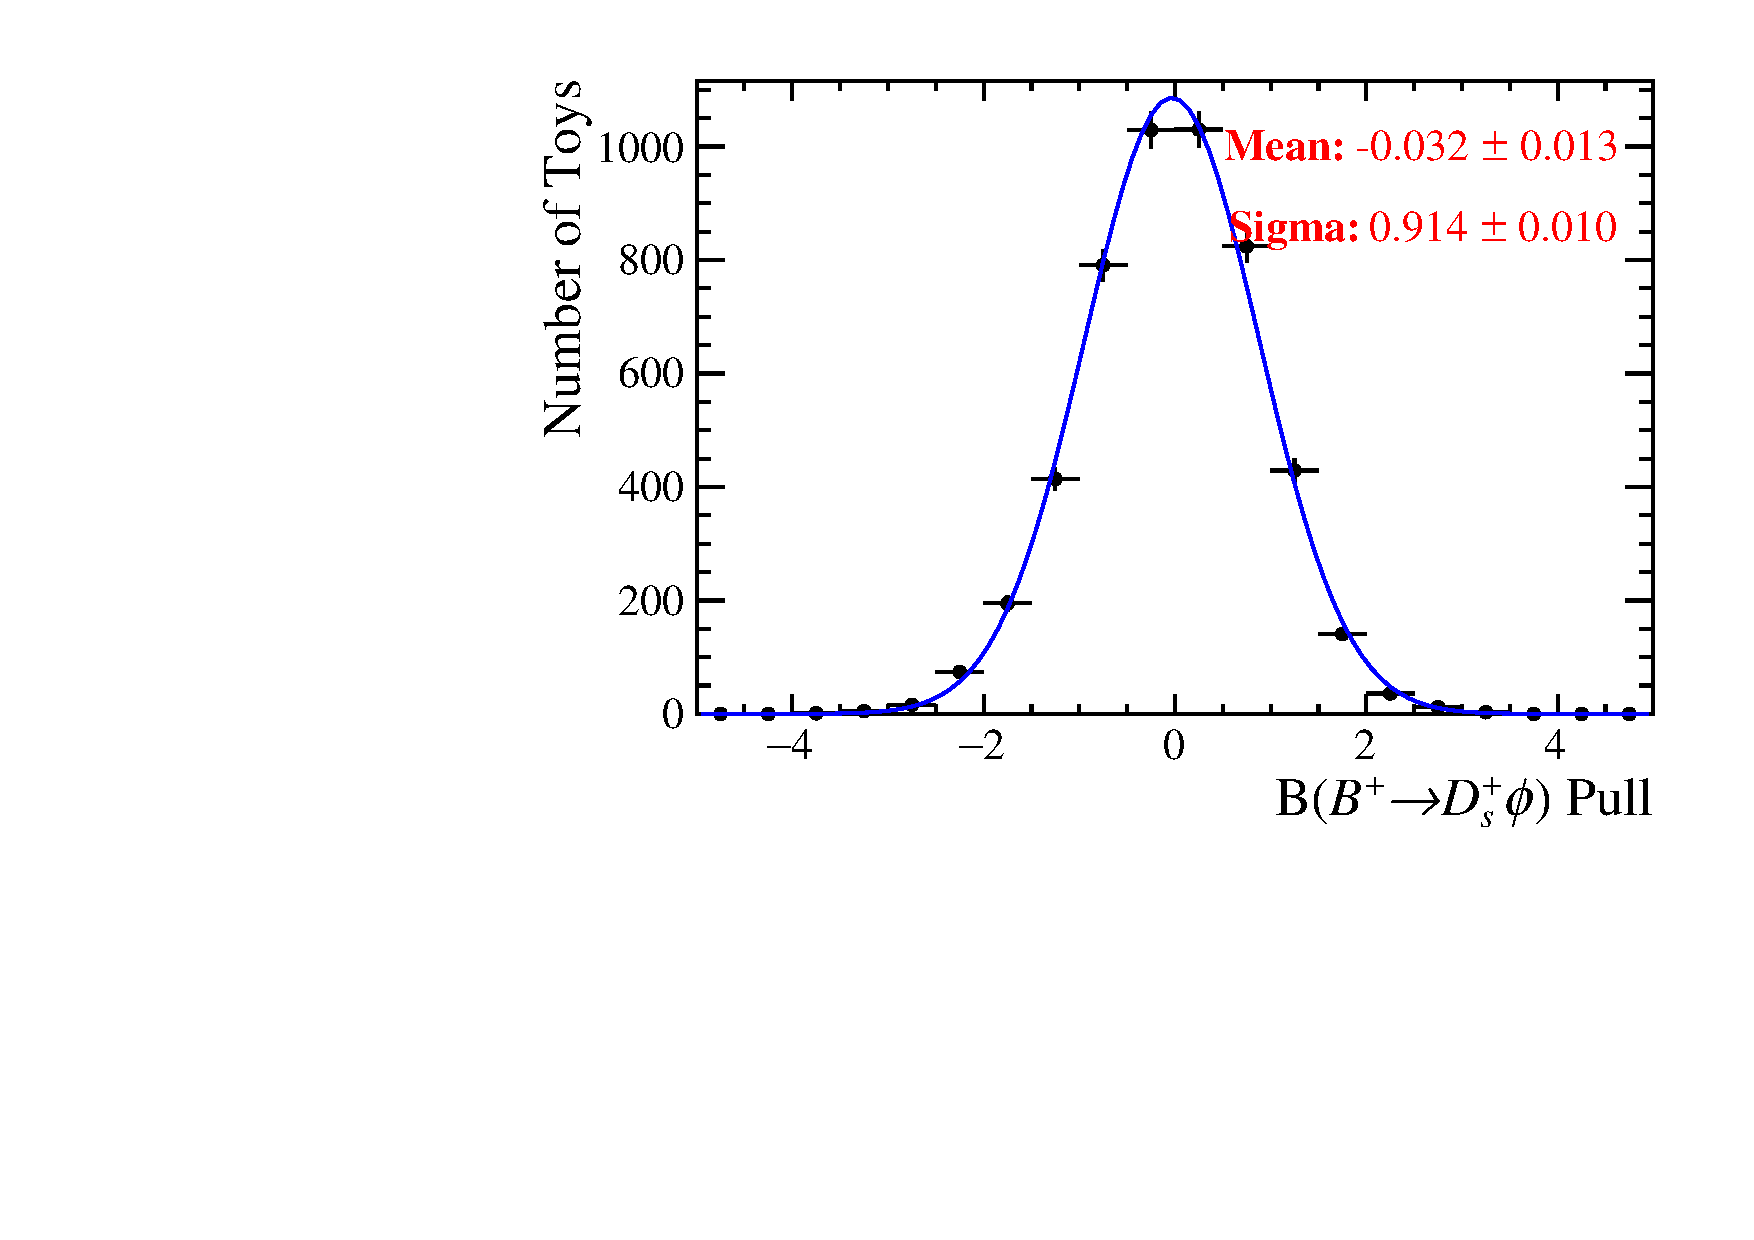
\includegraphics[width=0.32\textwidth]{figs/B2DsKK/Branching_Fraction_pul.pdf}
   \end{subfigure}\\
   \caption{The distribution of the branching fraction, error and pull as determined from pseudo-experiments. The result of fit performed to the pull distributions is overlaid in blue, along with the numerical results in red.}
   \label{fig:B2DsKK_BR_Pulls}
\end{figure}
%%%%%%%%%%%%%%%%%%%%%%%%%%%%%%%%%%%%%%%%%%%%%%%%%%%%%%%%%%

The pull in the branching fraction has a much smaller bias in the width than the normalisation pull.
It would be possible to scale the uncertainty in the branching fraction as determined by the fit to account for the residual bias in the uncertainty. However, this would introduce a source of systematic uncertainty associated to scaling factor so the choice is made to not correct the slightly overestimated uncertainty. 

\section{Normalisation and signal fits}

The signal and normalisation fits are performed using the model and dataset previously described. The results of the two fits are shown in Figs.~\ref{fig:B2DsKK_fit_B2DsD0} and \ref{fig:B2DsKK_fit_B2DsKK}. These figures shown the distribution of \Bp candidates along with the total model PDF constructed with the values of the free parameters determined in the NLL minimisation process. The contributions from each different component in the model are superimposed, stacked upon one another, and detailed in the legends.

%%%%%%%%%%%%%%%%%%%%%%%%%%%%%%%%%%%%%%%%%%%%%%%%%%%%%%%%%%
\begin{figure}[!h]
    \centering
    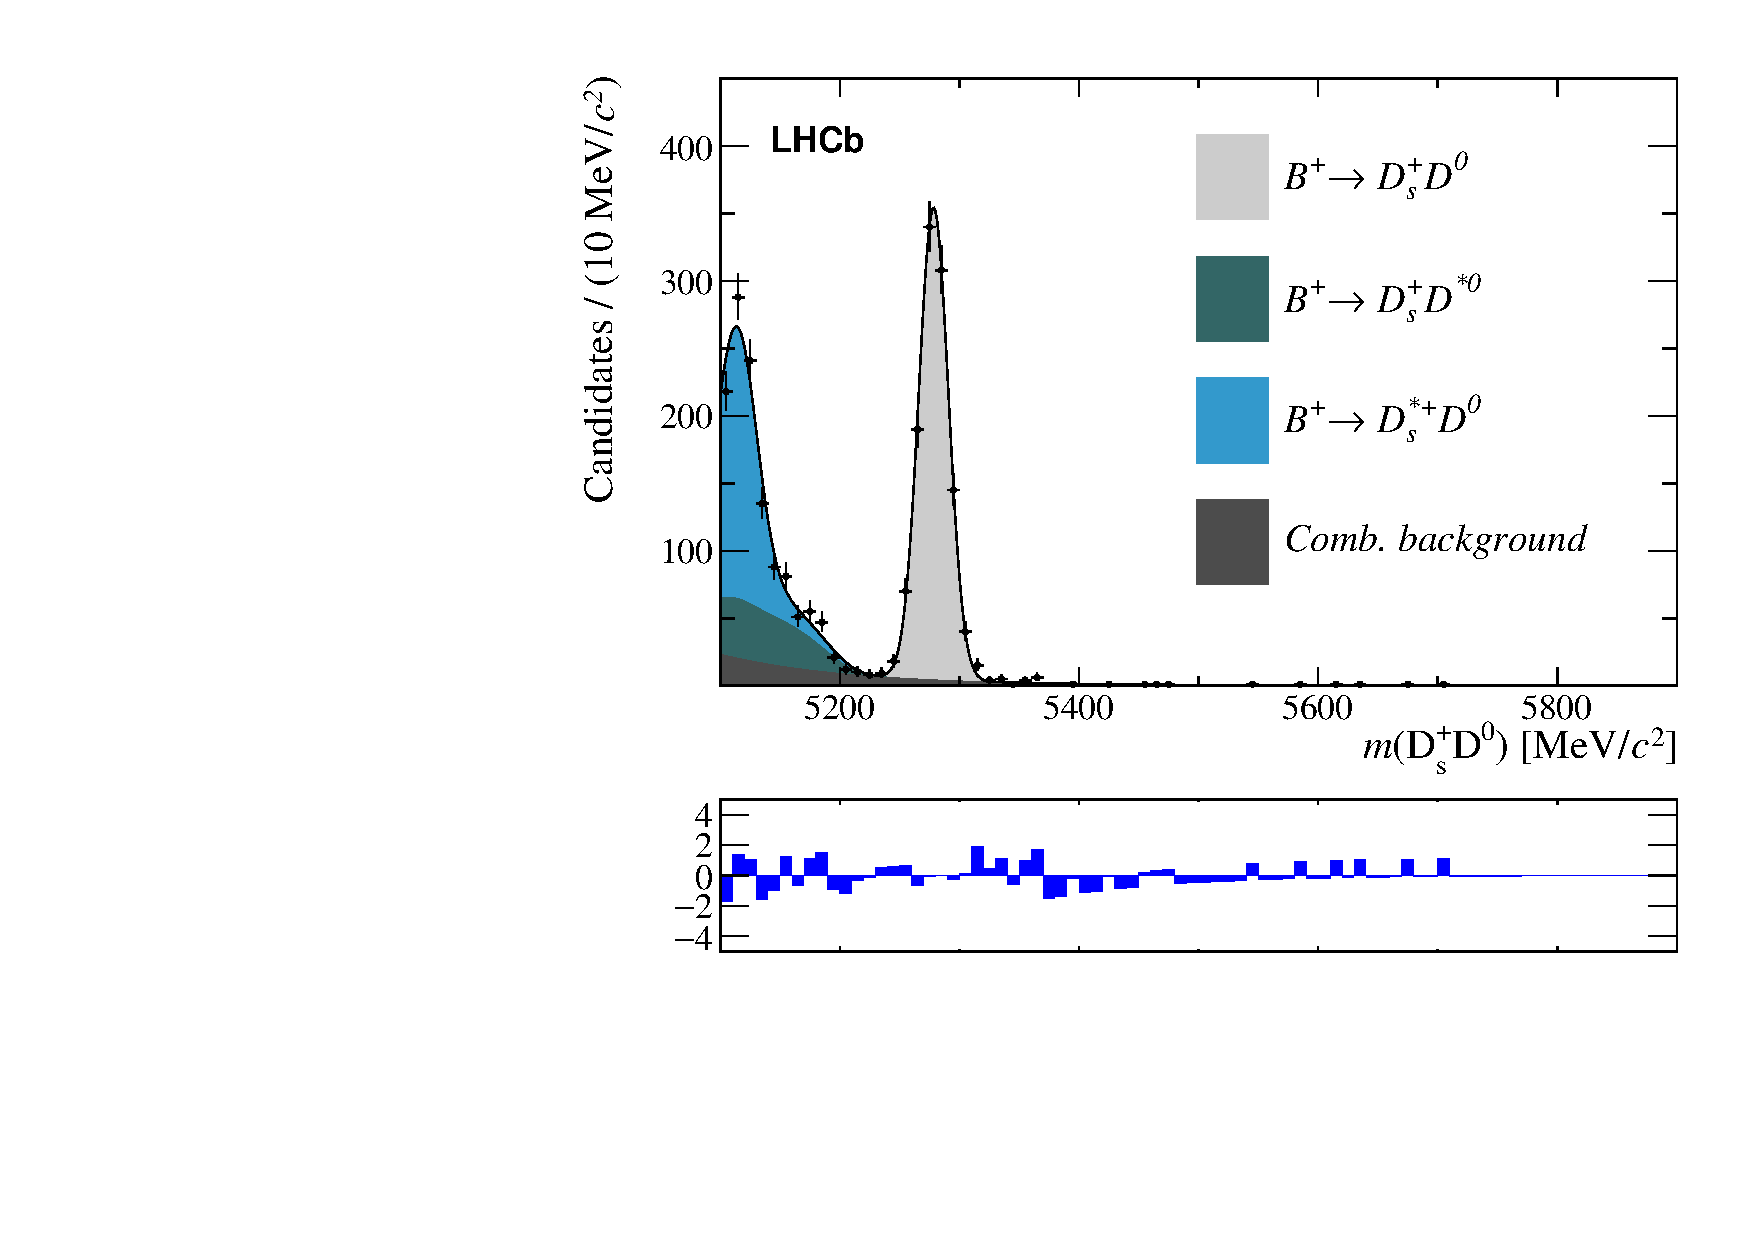
\includegraphics[width=0.8\textwidth]{figs/B2DsKK/Fit_DsD0.pdf}
    \caption{Invariant mass fit to \decay{\Bp}{\Dsp\Dzb} candidates.}
    \label{fig:B2DsKK_fit_B2DsD0}   
\end{figure}
%%%%%%%%%%%%%%%%%%%%%%%%%%%%%%%%%%%%%%%%%%%%%%%%%%%%%%%%%%

The distribution of \decay{\Bp}{\Dsp\Dzb} candidates in Fig.~\ref{fig:B2DsKK_fit_B2DsD0} demonstrates the relatively high purity of the selection. Additionally, there is a good separation between the normalisation peak and the partially reconstructed background. Only the combinatorial background is found to have a contribution at the same invariant mass as the normalisation peak. 


%%%%%%%%%%%%%%%%%%%%%%%%%%%%%%%%%%%%%%%%%%%%%%%%%%%%%%%%%%
\begin{figure}[!h]
    \centering
    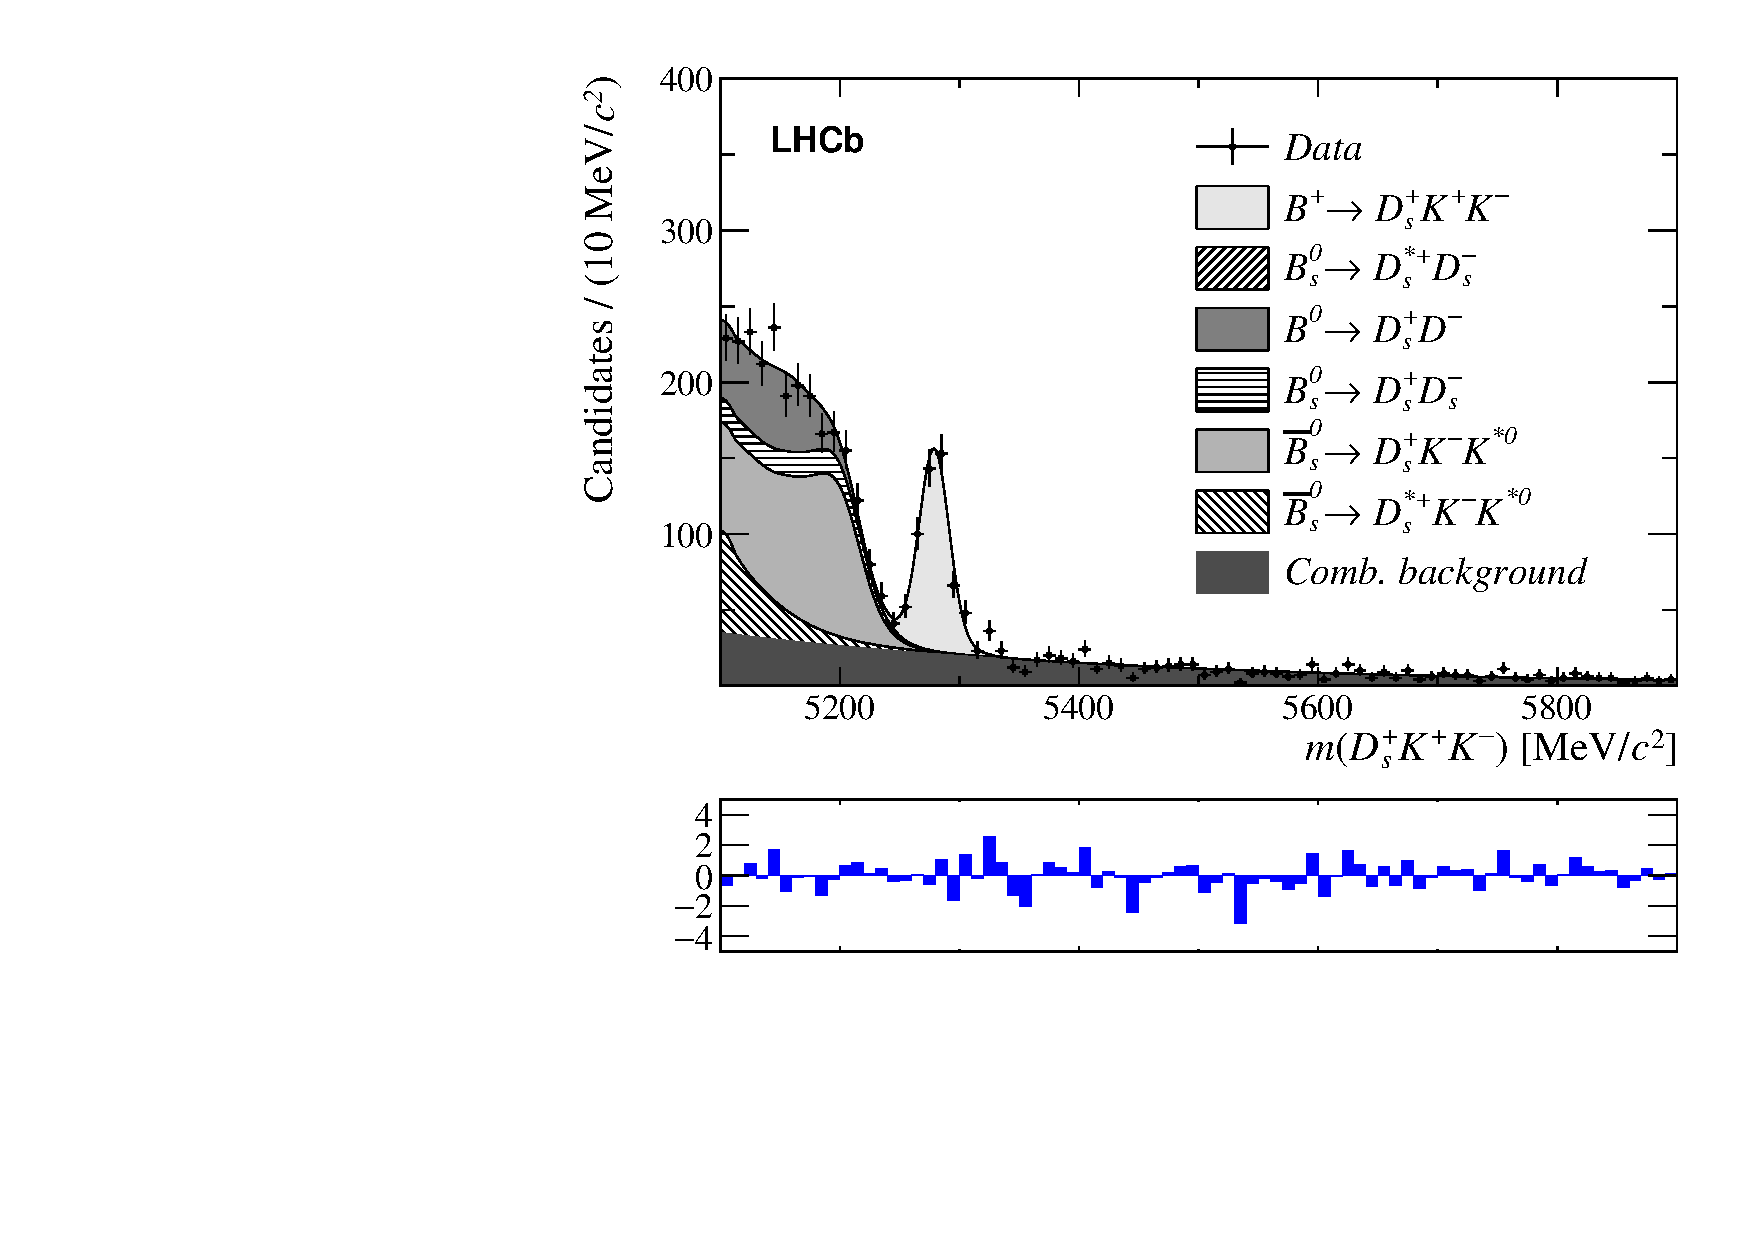
\includegraphics[width=0.8\textwidth]{figs/B2DsKK/Fit_DsKK.pdf}
    \caption{Invariant mass fit to \decay{\Bp}{\Dsp\Kp\Km} candidates.}
    \label{fig:B2DsKK_fit_B2DsKK}   
\end{figure}
%%%%%%%%%%%%%%%%%%%%%%%%%%%%%%%%%%%%%%%%%%%%%%%%%%%%%%%%%%

The distribution of \decay{\Bp}{\Dsp\Kp\Km} candidates shown in Fig.~\ref{fig:B2DsKK_fit_B2DsKK} has a significant contribution from the signal decay. The background contribution under the signal PDF is larger than was observed for the normalisation channel. Although the dominant background below the signal is still the combinatorial background, the contribution from the partially reconstructed backgrounds is also larger; several of the background PDFs extend underneath the leftmost half of the signal distribution.  


The numerical values of the free parameters determined in the fit to the signal and normalisation channels are listed in Tables~\ref{tab:B2DsKK_fit_result_norm} and \ref{tab:B2DsKK_fit_result_signal}.

\begin{table}[h]
    \centering
    \begin{tabular}{ l l c }
        \hline
        Type       & Parameter                                 & Fit result                         \\
        \hline
        POI         & $N(\decay{\Bp}{\Dsp\Dzb})$               & $1091\pm34$                \\

                  %         nsig    1.0905e+03    1.0905e+03 +/-  3.42e+01  <none>
        \hline
        Shape       & Mass shift $\delta$ (\mevcc)              & $-10.6\pm1.3$                 \\
                    & Relative peak heights $\xi$               & $0.0\pm0.2$                       \\
                    & Mean \Bp mass $\mu$ (\mevcc)              & $5278.4\pm0.4$                    \\
                    & Signal width $\sigma_{1}$ (\mevcc)        & $12.4\pm0.3$                      \\
                    & Combinatorial slope $c$                   & $(-9.4\pm1.1) \times 10^{-3}$     \\
                  %   global_csi    1.2683e-06    5.2233e-08 +/-  2.25e-01  <none>
                  % global_shift   -1.0585e+01   -1.0586e+01 +/-  1.31e+00  <none>
                  %       mean_B    5.2784e+03    5.2784e+03 +/-  4.00e-01  <none>
                  %        slope   -9.4305e-03   -9.4308e-03 +/-  1.13e-03  <none>
                  %        sigma    1.2436e+01    1.2435e+01 +/-  3.23e-01  <none>
        \hline
        Yields      & $N_{\text{comb}}$                         & $250\pm50$                        \\
                    & $N(\decay{\Bp}{\Dsp\Dstarzb})$            & $330\pm70$                        \\
                    & $N(\decay{\Bp}{\Dssp\Dzb})$               & $750\pm50$                        \\
                  %          nBG    2.4773e+02    2.4769e+02 +/-  5.42e+01  <none>
                  %      nDsDst0    3.3055e+02    3.3055e+02 +/-  6.72e+01  <none>
                  %      nDsstD0    7.5230e+02    7.5220e+02 +/-  5.48e+01  <none>
        \hline
    \end{tabular}  
    \caption{Normalisation fit result} 
    \label{tab:B2DsKK_fit_result_norm}
\end{table}
  

\begin{table}[h]
    \centering
    \begin{tabular}{ l l c }

        \hline
        Type        & Parameter                                 & Fit result                    \\
        \hline
        POI         & $N(\decay{\Bp}{\Dsp\Kp\Km})$              & $442\pm29$                    \\
                  %         nsig    4.4287e+02    4.4277e+02 +/-  2.94e+01  <none>
        \hline
        Shape       & Mass shift $\delta$ (\mevcc)              & $4\pm12$                      \\
                    & Mean \Bp mass $\mu$ (\mevcc)              & $5278.9\pm0.9$                \\
                    & Signal width $\sigma_{1}$ (\mevcc)        & $12.3\pm0.9$                  \\
                    & Combinatorial slope $c$                   & $(-2.8\pm0.3) \times 10^{-3}$ \\
                  % global_shift    2.2538e+00    3.5457e+00 +/-  1.17e+01  <none>
                  %       mean_B    5.2789e+03    5.2789e+03 +/-  8.82e-01  <none>
                  %        sigma    1.2298e+01    1.2291e+01 +/-  8.77e-01  <none>
                  %        slope   -2.8199e-03   -2.8202e-03 +/-  2.79e-04  <none>
        \hline
        Yields      & $N_{\text{comb}}$                         & $1110\pm70$                   \\
                    & $N(\decay{\Bsb}{\Dsp\Km\Kstarz})$         & $1100\pm500$                  \\
                    & $N(\decay{\Bsb}{\Dssp\Km\Kstarz})$        & $300\pm120$                   \\
                    & $N(\decay{\Bs}{\Dsp\Dsm})$                & $200\pm500$                   \\
                    & $N(\decay{\Bz}{\Dsp\Dm})$                 & $470\pm150$                   \\
                    & $N(\decay{\Bs}{\Dssp\Dsm})$               & $0\pm400$                     \\
                  %          nBG    1.1139e+03    1.1142e+03 +/-  7.30e+01  <none>
                  %     nBs2Dsa1    1.1153e+03    1.1147e+03 +/-  4.61e+02  <none>
                  % nBs2DsstKKst    2.9756e+02    2.9691e+02 +/-  1.24e+02  <none>
                  %     nBs2DsDs    2.0262e+02    2.0307e+02 +/-  5.08e+02  <none>
                  %      nB02DsD    4.6587e+02    4.6621e+02 +/-  1.54e+02  <none>
                  %   nBs2DsstDs    1.1208e-04    6.2385e-02 +/-  3.98e+02  <none>
        \hline
    \end{tabular}  
    \caption{Signal fit result} 
    \label{tab:B2DsKK_fit_result_signal}
\end{table}



Two of the common parameters between the two modes, namely the mean \Bp mass and width, have consistent values between the two fits. The combinatorial slopes vary between the two, likely because of the different background levels in the two datasets. Similarly the mass shifts vary between the two. 

\section{Efficiency corrections}
\label{sec:B2DsKK_effcorrection}

The branching fraction for \decay{\Bp}{\Dsp\Kp\Km} decays is determined by correcting the yields of signal and background decays by their corresponding selection efficiencies. These account for each step of the selection process and ultimately quantifies the extent to which the signal and normalisation channels are affected differently. As described in Sec.~\ref{sec:B2DsKK_fitstrategy} the signal yield is corrected by the efficiency as a function of the candidate's kinematic properties. Therefore the relative signal efficiency is determined as a function of the two-dimensional Dalitz plot coordinates $m^{2}(\Dsp\Km)$ and $m^{2}(\Kp\Km)$
\begin{equation}
\epsilon_{\text{ratio}}(m^{2}(\Dsp\Km),m^{2}(\Kp\Km)) = \frac{\epsilon_{\decay{\Bp}{\Dsp\Kp\Km}}(m^{2}(\Dsp\Km),m^{2}(\Kp\Km))}{\epsilon_{\decay{\Bp}{\Dsp\Dzb}}}.
\end{equation}
The normalisation decay efficiency $\epsilon_{\decay{\Bp}{\Dsp\Dzb}}$ is a pseudo-two-body decay and therefore the efficiency has no dependence on the phase space coordinates. The kinematic phase space is split into bins and the efficiencies determined in each. 


The efficiencies are all determined using samples of simulated signal and normalisation decays. The PID and MVA efficiencies require additional input from external calibration samples to correct for the imperfect modelling of the PID variables in the simulations.

{\color{Red}
\begin{itemize}
\item add total equation for efficiency? 
\end{itemize}
}

\subsection{Efficiencies from simulations} 

\begin{description}
\item \textbf{Acceptance:} this accounts for the likelihood for the five final state tracks to be within the \lhcb detector's acceptance. The charged tracks are required to be in the range $10 < \cos\theta < 400 \mrad$, where $\theta$ is the angle between the beam direction and the track. The relative efficiency is shown as a function of the \decay{\Bp}{\Dsp\Kp\Km} Dalitz plot in Fig.\ref{fig:B2DsKK_releff_acceptance}. The relative efficiency is close to one for most of the phase-space. 

\item \textbf{Reconstruction:} the reconstruction efficiency accounts for the fraction of decays in which all five final state tracks have been correctly reconstructed and combined into a \Bp candidate that passes all selection requirements outlined in the \decay{\Bp}{\Dsp\Kp\Km} \emph{Stripping Line}. The \emph{Stripping Line} reconstruction also explicitly requires that at least one trigger has fired for the event to be reconstructed, therefore this efficiency also account for part of the trigger efficiency. The distribution of the relative reconstruction efficiency between the signal and normalisation mode is shown in Fig.~\ref{fig:B2DsKK_releff_reconstruction}. This is greater than one across the whole phase-space as a result of the choice to reconstruct the \decay{\Bp}{\Dsp\Dzb} normalisation decays using the same selection as the \decay{\Bp}{\Dsp\Kp\Km} signal. The latter requires the \Dsp, \Kp and \Km candidates to form a well reconstructed vertex where the \Bp meson decays. However, for the normalisation channel the \Dzb meson travels away from this vertex, so some of the longer lived \Dzb candidates do not pass the vertex quality requirement. This reduces the efficiency for the normalisation channel relative to the signal.

\end{description}
%%%%%%%%%%%%%%%%%%%%%%%%%%%%%%%%%%%%%%%%%%%%%%%%%%%%%%%%%%
\begin{figure}[!h]
   \centering
   \begin{subfigure}[t]{0.4\textwidth}
      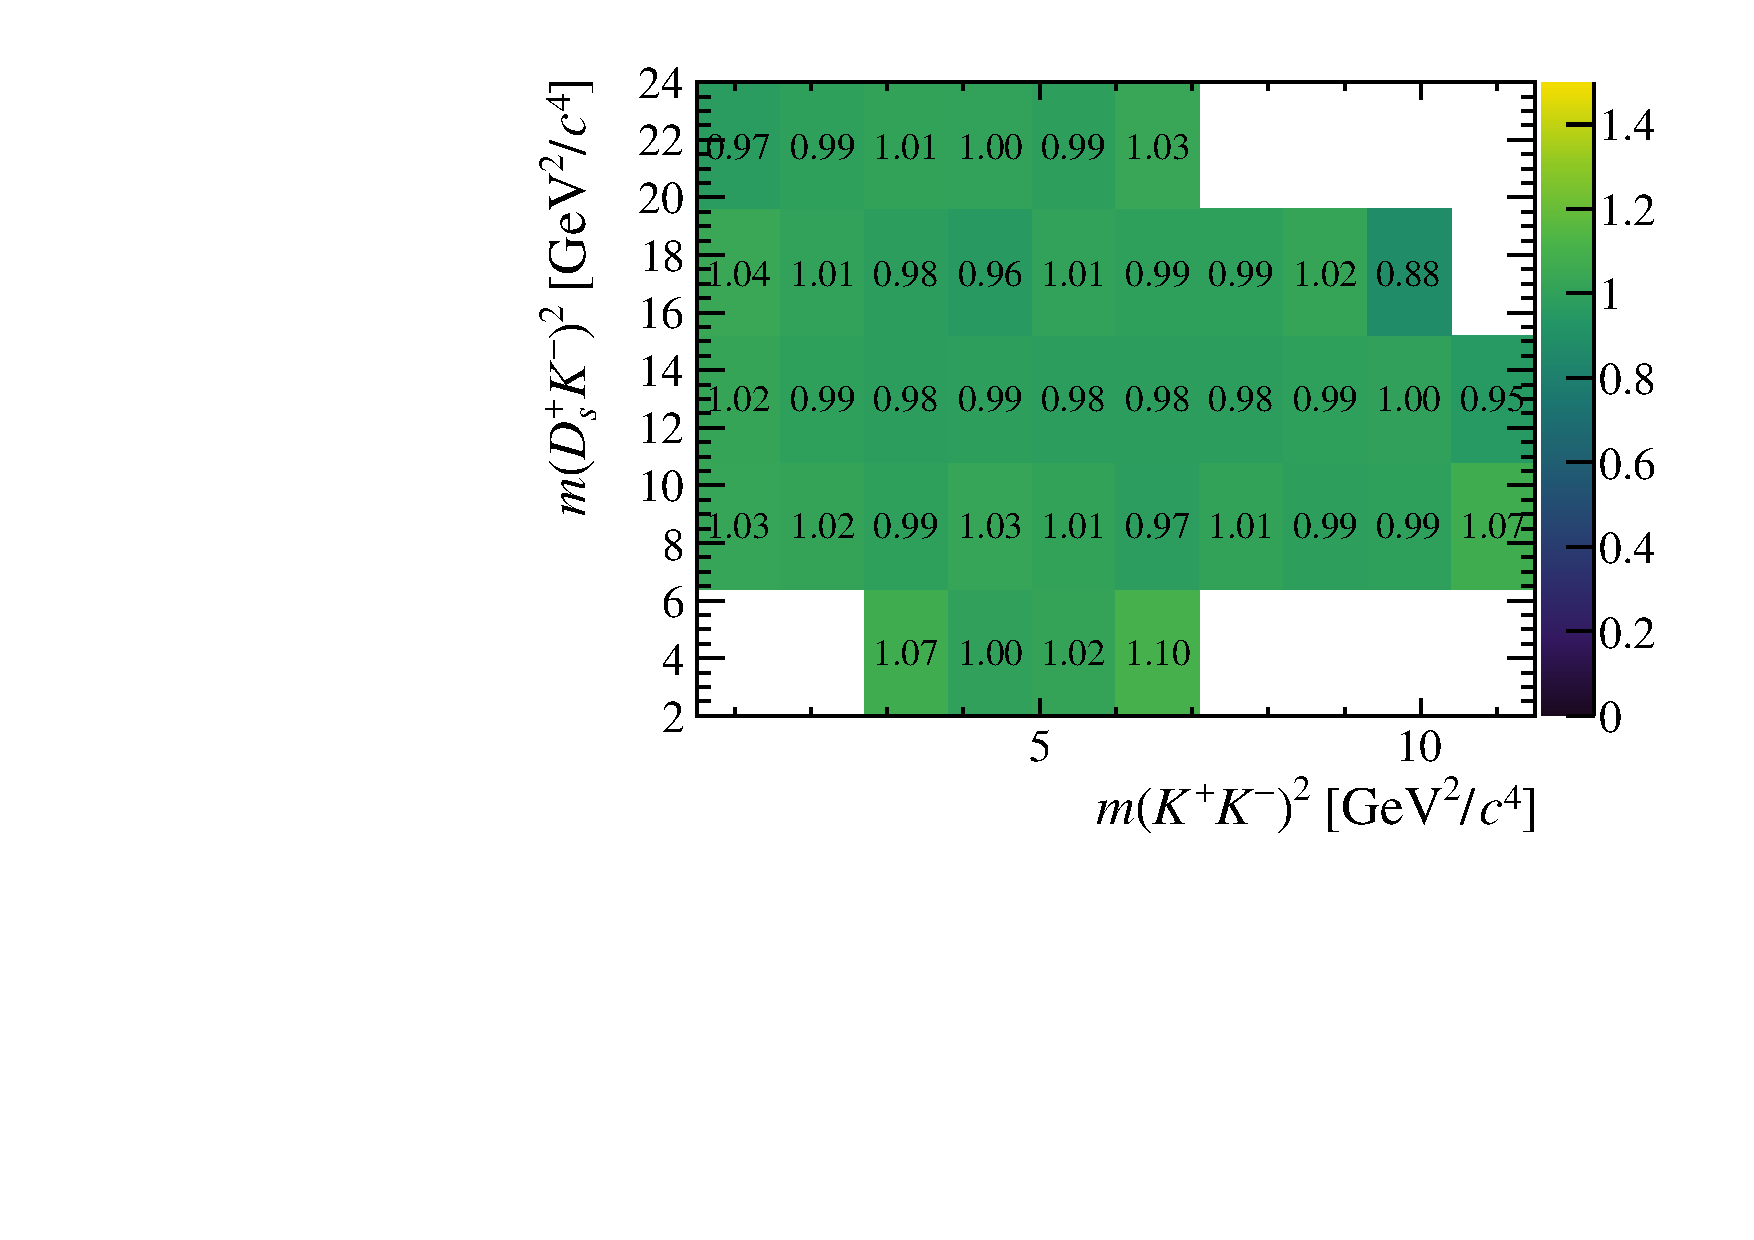
\includegraphics[width=1.0\textwidth]{figs/B2DsKK/Relative_Eff_gen_All_Full.pdf}
      \caption{Acceptance}
      \label{fig:B2DsKK_releff_acceptance}
   \end{subfigure}
   \begin{subfigure}[t]{0.4\textwidth}
      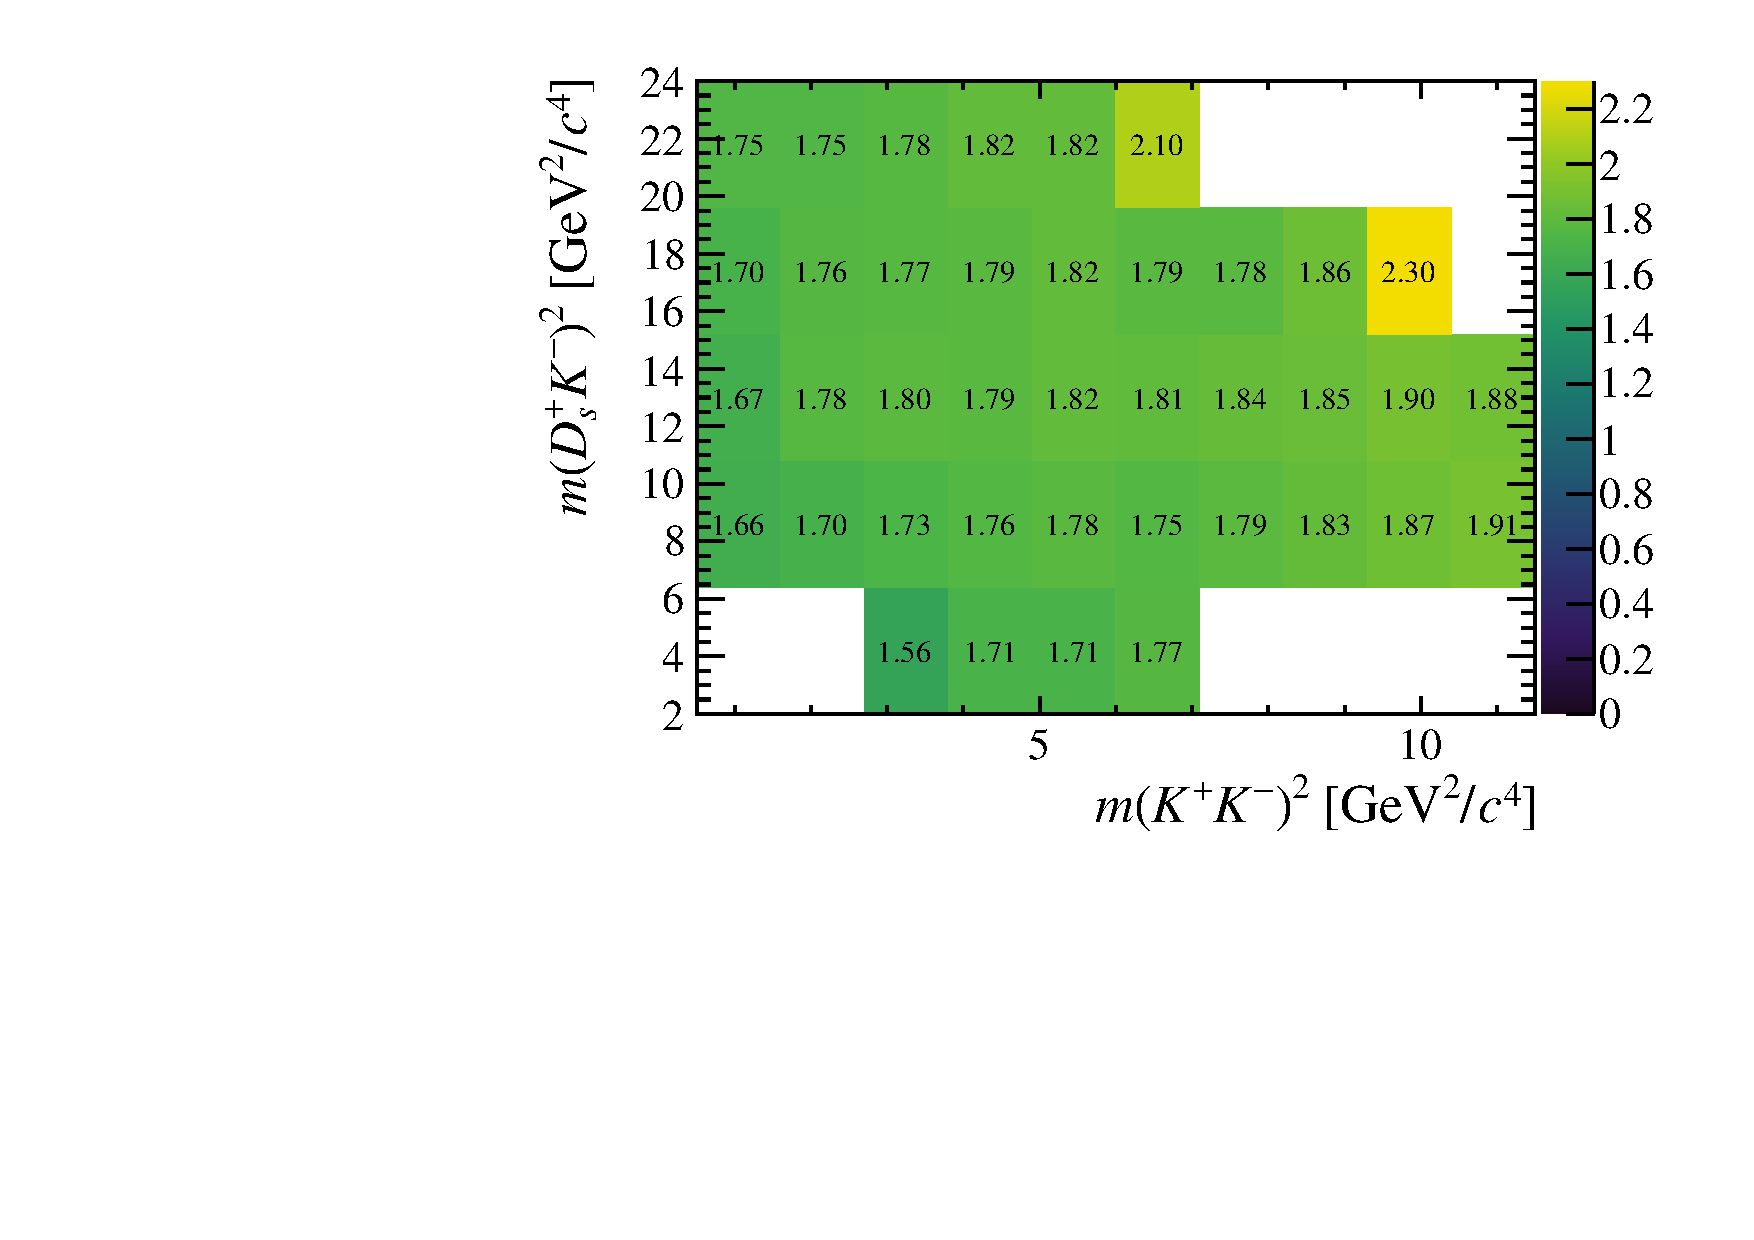
\includegraphics[width=1.0\textwidth]{figs/B2DsKK/Relative_Eff_reco_All.pdf}
      \caption{Reconstruction}
      \label{fig:B2DsKK_releff_reconstruction}
   \end{subfigure}
   \caption{The relative efficiency $\epsilon_{\text{ratio}}(m^{2}(\Dsp\Km),m^{2}(\Kp\Km))$ as a function of the \decay{\Bp}{\Dsp\Kp\Km} kinematics.}
   \label{fig:B2DsKK_dalitz_eff_one}
\end{figure}
%%%%%%%%%%%%%%%%%%%%%%%%%%%%%%%%%%%%%%%%%%%%%%%%%%%%%%%%%%


\begin{description}
\item \textbf{Trigger:} the trigger efficiency accounts for the fraction of decays for which the signal candidate meets the \texttt{TIS} and \texttt{TOS} requirements outlined in Sec.~\ref{sec:selection_trigger}, given that the trigger fired in that event. For the signal and normalisation simulation samples it is very likely that the signal candidate was the cause of the trigger if a trigger fired, therefore these are typically around 95\%. The phase-space distribution of the relative efficiency is very uniform and shown in Fig.~\ref{fig:B2DsKK_releff_trigger}.
\item \textbf{Vetoes:} this efficiency accounts for the fraction of decays passing the kinematic and normalisation vetoes detailed in Sec.~\ref{sec:kinematicvetos} and \ref{sec:normvetos}. The vetoes to remove misidentified \D and \Lc hadrons are only applied to the \Dsp meson and therefore assumed to affect the signal and normalisation mode equally. The systematic uncertainty arising from this choice is discussed in Sections~\ref{sec:B2DsKK_sys_releff}. Although the veto for misidentified normalisation decays proceeding via \decay{\Dzb}{\Kp\pim} decays is included, the veto to remove correctly reconstructed normalisation decays with \decay{\Dzb}{\Kp\Km} is not included. This is because the width of this veto is less that the binning width so it would therefore lead to the wrong efficiency for candidates within in the same bin but not in the window. This doesn't affect the final result, it simply means areas of the efficiency Dalitz plot are populated that will never be sampled. The distribution of the relative efficiency is shown in Fig.~\ref{fig:B2DsKK_releff_vetoes}. A vertical band is clear in the centre as a result of the veto for misidentified normalisation decays with \decay{\Dzb}{\Kp\pim}.
\end{description}

%%%%%%%%%%%%%%%%%%%%%%%%%%%%%%%%%%%%%%%%%%%%%%%%%%%%%%%%%%
\begin{figure}[!h]
   \centering
   \begin{subfigure}[t]{0.4\textwidth}
      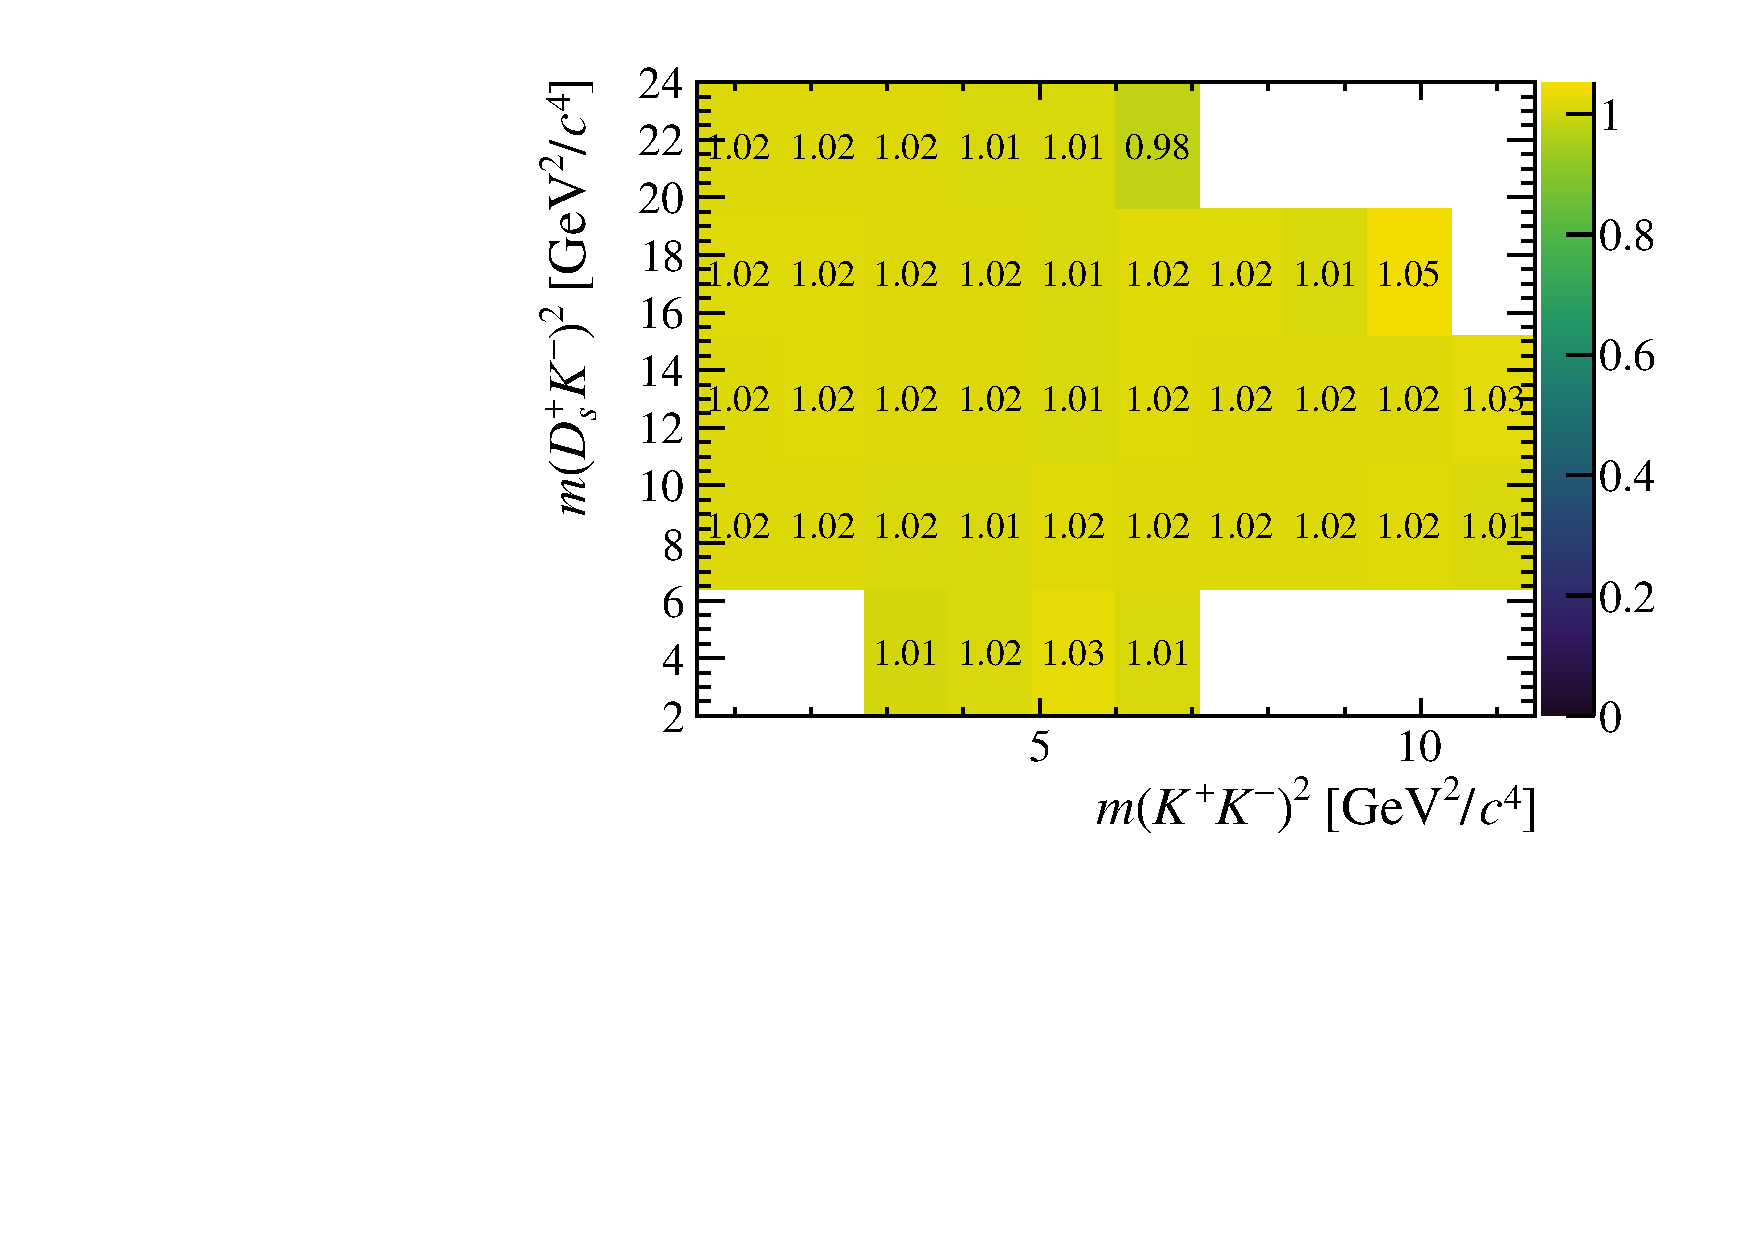
\includegraphics[width=1.0\textwidth]{figs/B2DsKK/Relative_Eff_trig_All.pdf}
      \caption{Trigger}
      \label{fig:B2DsKK_releff_trigger}
   \end{subfigure}
   \begin{subfigure}[t]{0.4\textwidth}
      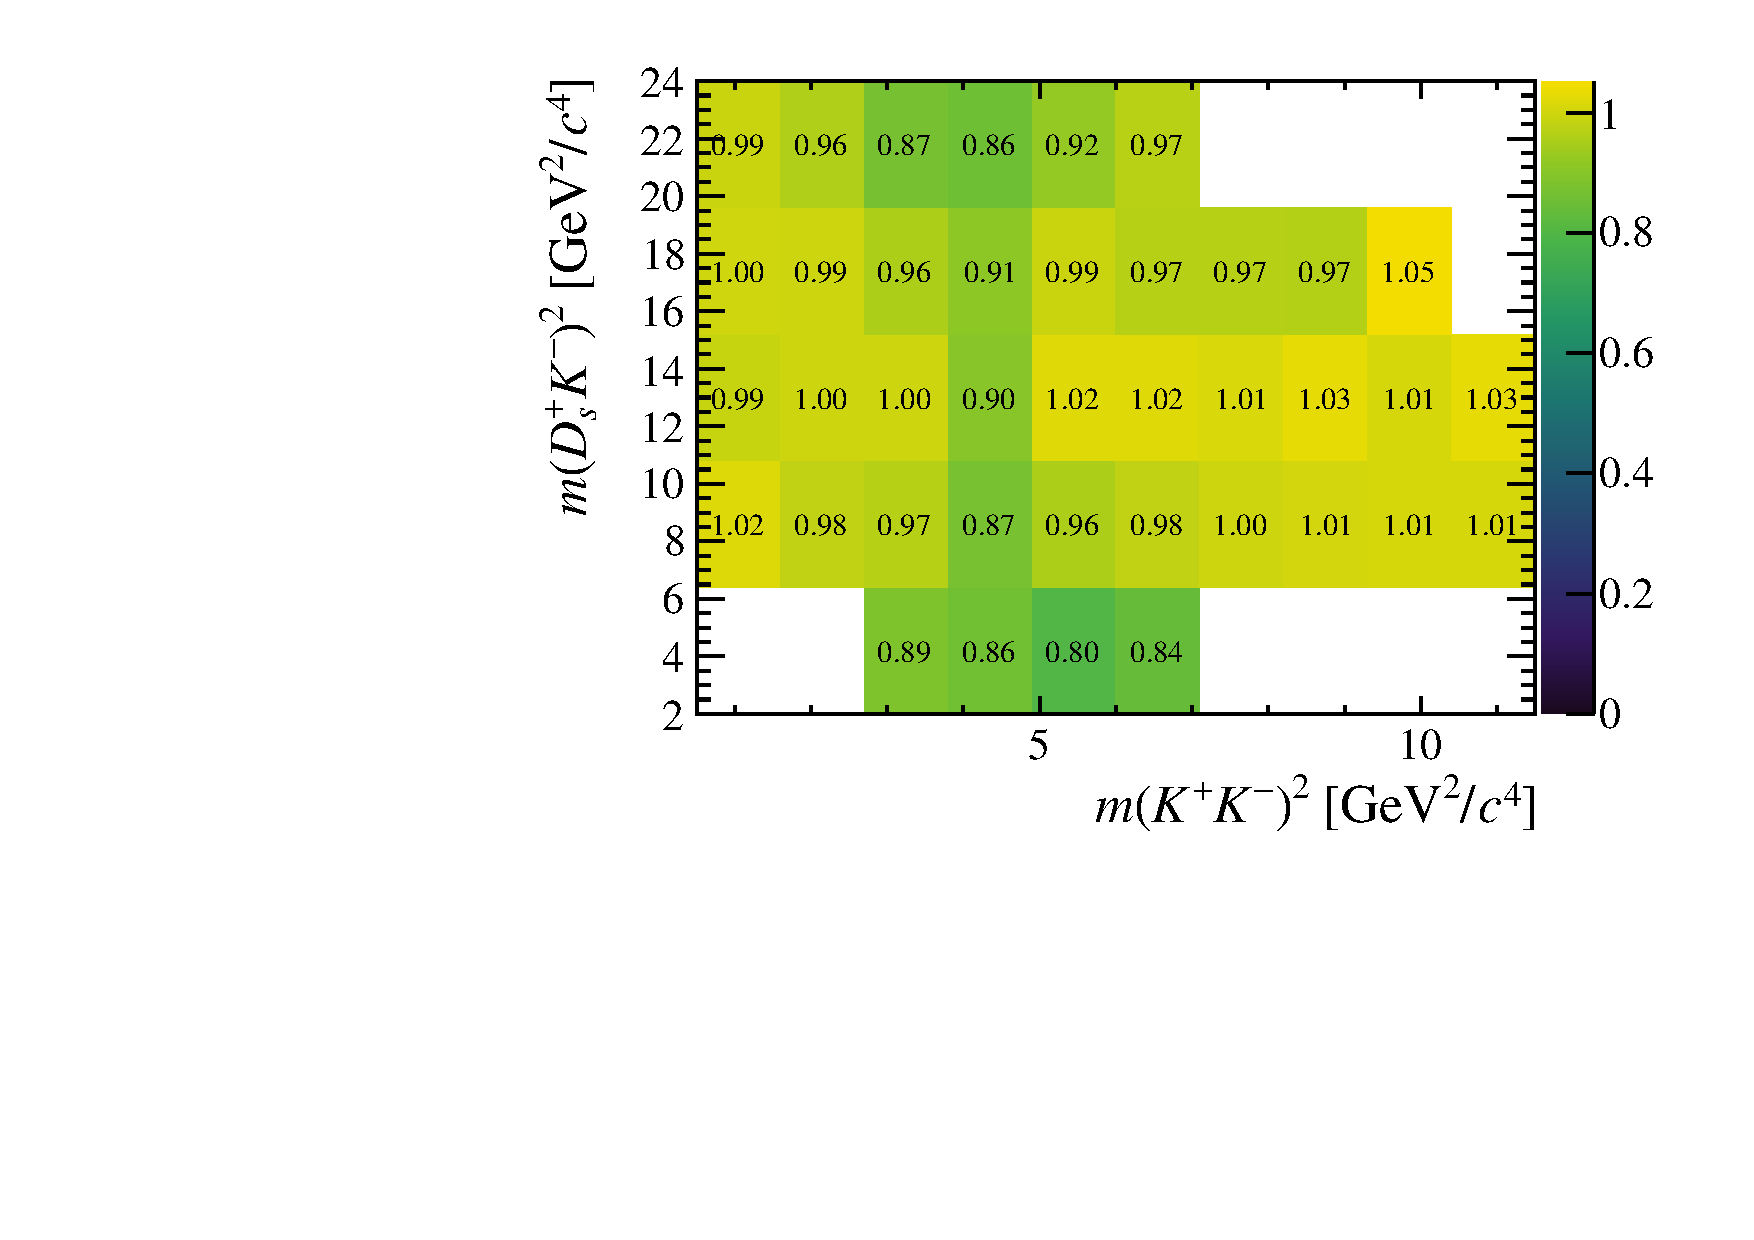
\includegraphics[width=1.0\textwidth]{figs/B2DsKK/Relative_Eff_veto_All.pdf}
      \caption{Vetoes}
      \label{fig:B2DsKK_releff_vetoes}
   \end{subfigure}
   \caption{The relative efficiency $\epsilon_{\text{ratio}}(m^{2}(\Dsp\Km),m^{2}(\Kp\Km))$ as a function of the \decay{\Bp}{\Dsp\Kp\Km} kinematics.}
   \label{fig:B2DsKK_dalitz_eff_one}
\end{figure}
%%%%%%%%%%%%%%%%%%%%%%%%%%%%%%%%%%%%%%%%%%%%%%%%%%%%%%%%%%

\begin{description}

\item \textbf{Charmless:} this accounts for the fraction of decays failing the requirements on the \D meson flight distance requirements aimed at removing charmless and single-charm backgrounds. The distribution shown in Fig.\ref{fig:B2DsKK_releff_charmless} shows a fairly flat distribution with the exception of some of the edge bins.
\item \textbf{$\chi^{2}_{\text{IP}}$:} this accounts for the fraction of decays that pass the requirements on the \Bp and \Dsp meson impact parameter significance. The relative efficiency is shown in Fig.~\ref{fig:B2DsKK_releff_ipchi2} and shows a strong dependency on phase-space at high $m^{2}(\Kp\Km)$. The lower relative efficiencies at high $m^{2}(\Kp\Km)$ may be because the \Dp meson is produced almost at rest in this region. Therefore these \Dsp mesons are likely to have a lower momentum and may fail the minimum impact parameter significance requirement.
\end{description}

%%%%%%%%%%%%%%%%%%%%%%%%%%%%%%%%%%%%%%%%%%%%%%%%%%%%%%%%%%
\begin{figure}[!h]
   \centering
   \begin{subfigure}[t]{0.4\textwidth}
      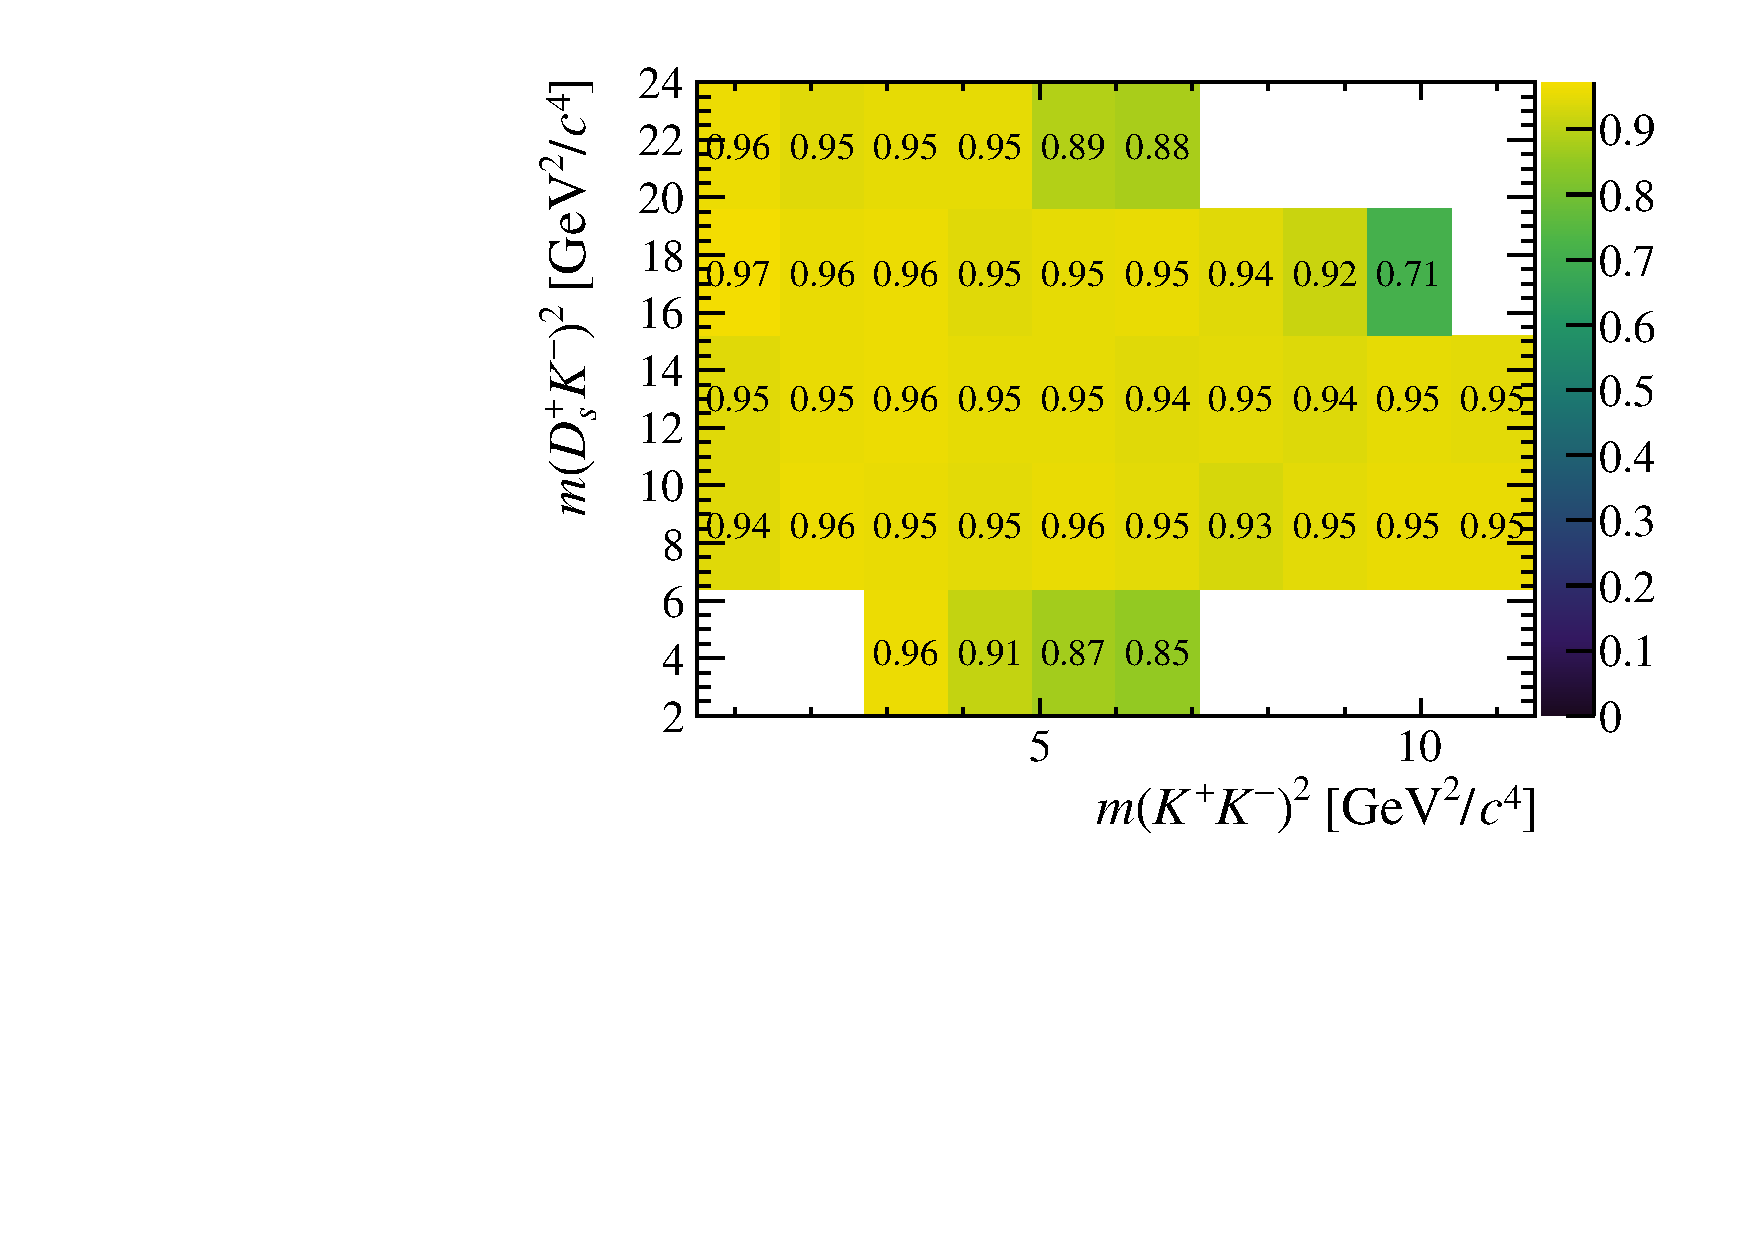
\includegraphics[width=1.0\textwidth]{figs/B2DsKK/Relative_Eff_FDCHI2_All.pdf}
      \caption{Charmless}
      \label{fig:B2DsKK_releff_charmless}
   \end{subfigure}
   \begin{subfigure}[t]{0.4\textwidth}
      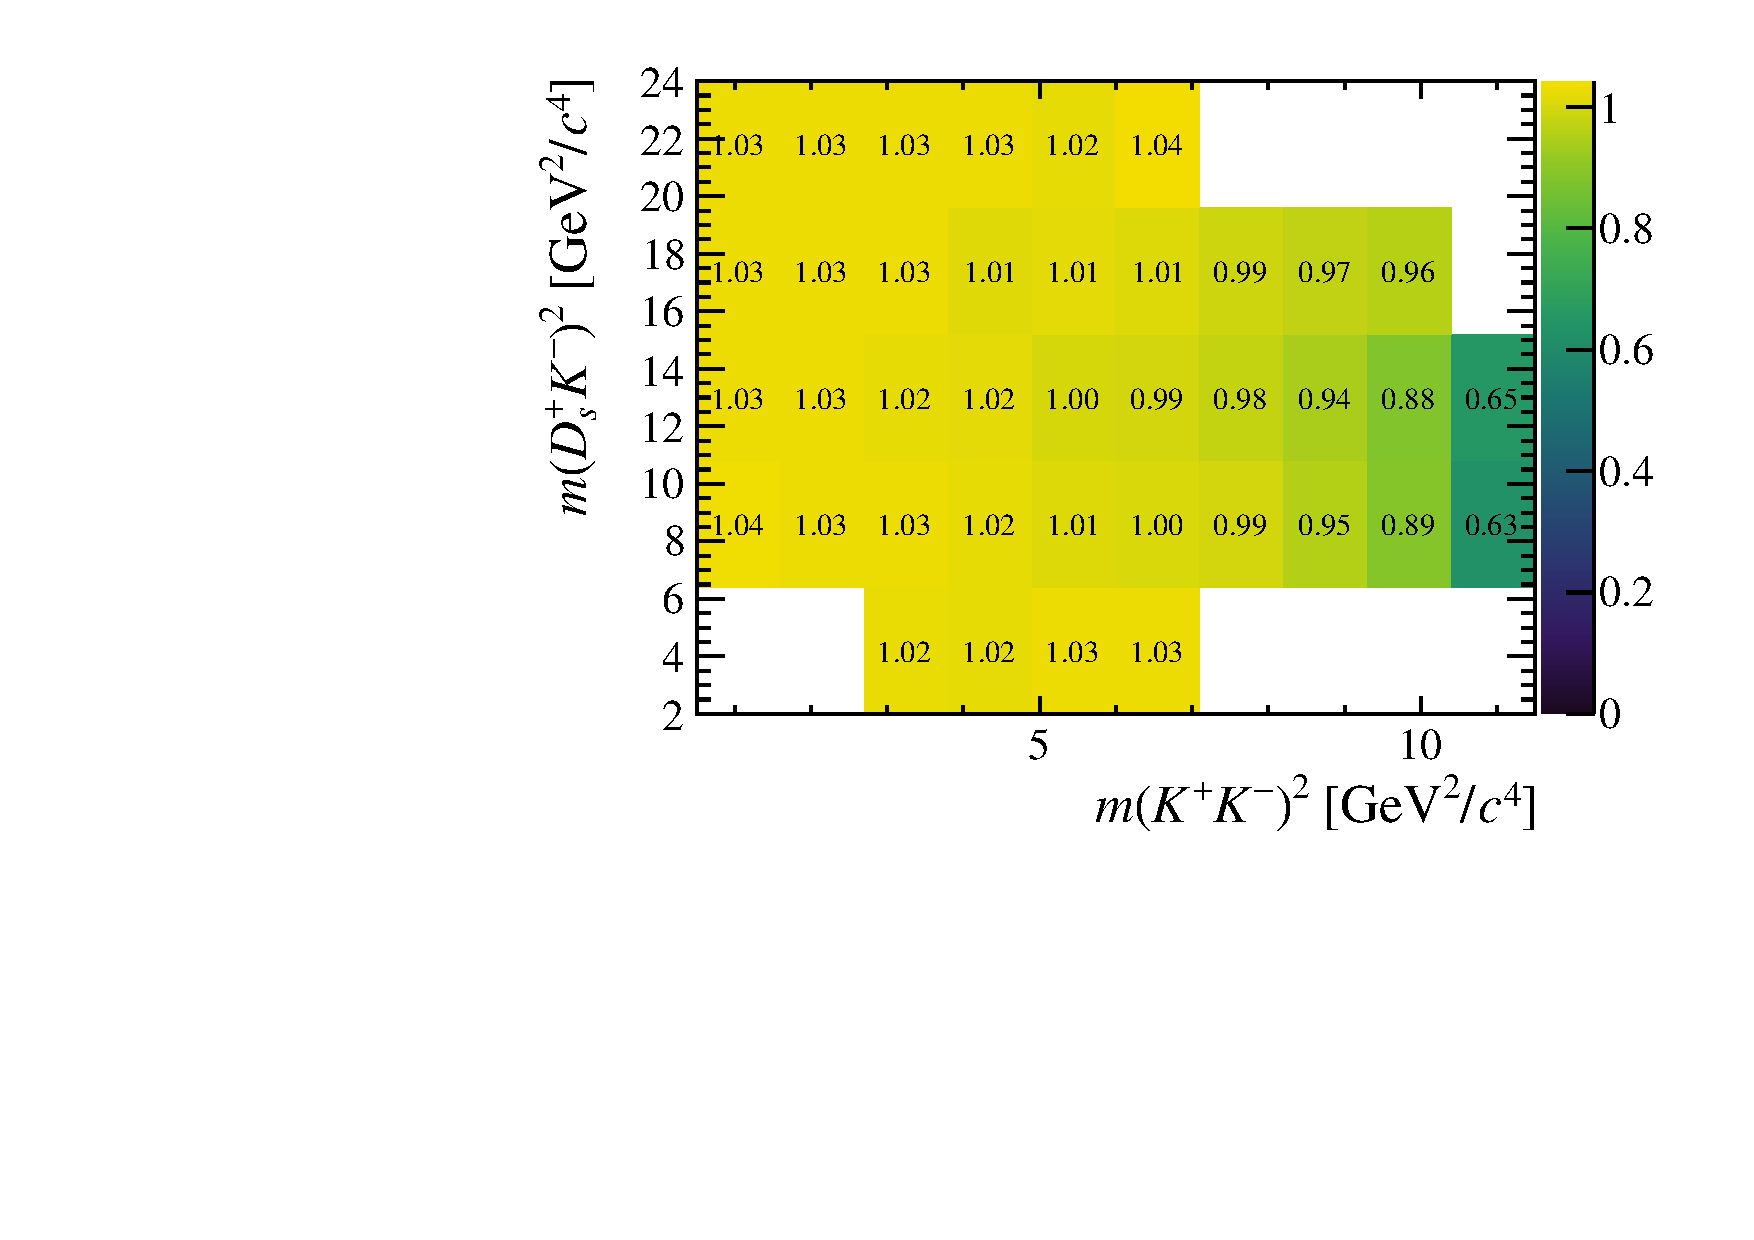
\includegraphics[width=1.0\textwidth]{figs/B2DsKK/Relative_Eff_Bcut_All.pdf}
      \caption{$\chi^{2}_{\text{IP}}$}
      \label{fig:B2DsKK_releff_ipchi2}
   \end{subfigure}
   \caption{The relative efficiency $\epsilon_{\text{ratio}}(m^{2}(\Dsp\Km),m^{2}(\Kp\Km))$ as a function of the \decay{\Bp}{\Dsp\Kp\Km} kinematics.}
   \label{fig:B2DsKK_dalitz_eff_two}
\end{figure}
%%%%%%%%%%%%%%%%%%%%%%%%%%%%%%%%%%%%%%%%%%%%%%%%%%%%%%%%%%

\begin{description}
\item \textbf{Mass windows:} this accounts for the fraction of decays that pass the mass windows around the \Dsp and \Dzb masses. No requirement is placed on the \Kp\Km pair, therefore the relative efficiency shown in Fig.~\ref{fig:B2DsKK_releff_masswindows} is slightly greater than one across the whole phase-space. 
\end{description}



%%%%%%%%%%%%%%%%%%%%%%%%%%%%%%%%%%%%%%%%%%%%%%%%%%%%%%%%%%
\begin{figure}[!h]
   \centering
   \begin{subfigure}[t]{0.4\textwidth}
      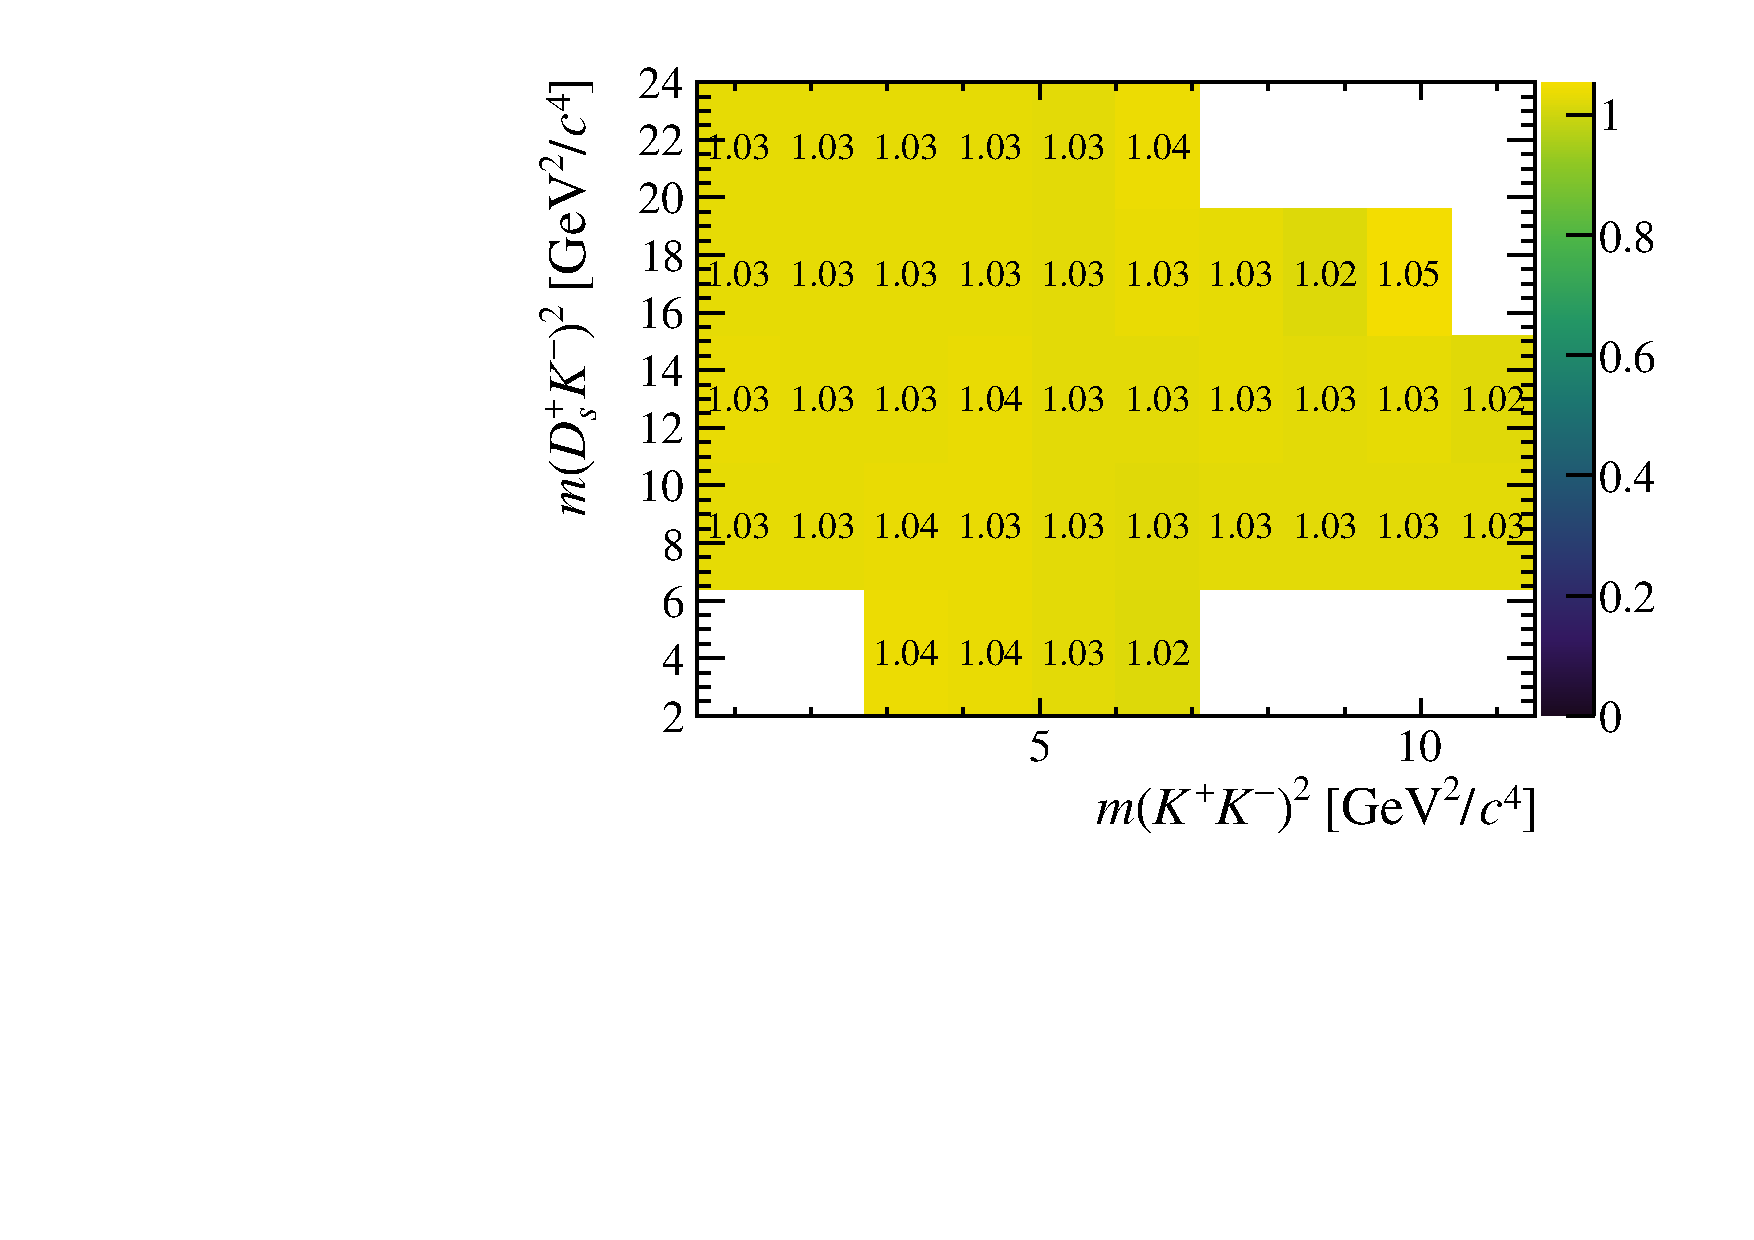
\includegraphics[width=1.0\textwidth]{figs/B2DsKK/Relative_Eff_mass_All.pdf}
      \caption{Mass windows}
      \label{fig:B2DsKK_releff_masswindows}
   \end{subfigure}
   \caption{The relative efficiency $\epsilon_{\text{ratio}}(m^{2}(\Dsp\Km),m^{2}(\Kp\Km))$ as a function of the \decay{\Bp}{\Dsp\Kp\Km} kinematics.}
   \label{fig:B2DsKK_dalitz_eff_two}
\end{figure}
%%%%%%%%%%%%%%%%%%%%%%%%%%%%%%%%%%%%%%%%%%%%%%%%%%%%%%%%%%


\subsection{Efficiencies requiring calibration samples} 
\label{sec:B2DsKK_eff_from_calib}

\subsubsection{PID efficiency}
The efficiencies for the particle identification requirements as described in Sec.~\ref{sec:pidrequirements} are calculated by correcting the PID variables in simulation using a package called \pidcalib~\cite{PIDCalib}. This uses calibrations samples for the different particle species to determine the distribution of the PID variables in data. The calibration samples are background-subtracted to isolate the distributions of the PID variables for the tracks of interest. The calibration samples for both \Kp and \pip mesons are collected from samples of \decay{\Dstarp}{(\decay{\Dz}{\Kp\pim})\pip} decays, using the decay products of the \Dz decay. Additionally, samples of protons are collected from \decay{\PLambda}{\proton\pim} decays. The PID variable distributions depend on both the kinematics of the track in question and the occupancy of the detector as a whole. These can both affect the characteristics of the hits in the \rich sub-detectors and therefore result in different PID variable distributions. The calibrations samples are characterised using three variables; the transverse momentum of the track \pt, the pseudo-rapidity \Peta, and the number of tracks in an event $n_{\text{Tracks}}$. 
The calibration PID variables are parametrised using an unbinned approach, unlike in the search for \decay{\Bp}{\Dsp\phiz} where a binned approach is used (Sec.~\ref{sec:B2DsPhi_eff_PID}). This unbinned approach creates four dimensional PDFs (PID,\Peta,\pt,$n_{\text{Tracks}}$) from the calibration samples using a kernel density estimation implemented with the \meerkat package~\cite{Meerkat}. Similar four dimensional PDFs are created for simulation samples of the calibration modes. These two PDFs are used to calculate the transformation needed for each species as a function of (PID,\Peta,\pt,$n_{\text{Tracks}}$) to correct the distribution in simulation. 
This transformation preserves the correlations between the different PID variables and between the PID and kinematic properties. 
This correction is applied to both the DLL PID variables and ProbNNx variables used in the MVA selection. 
The phase-space distribution of the relative PID efficiency between the signal and normalisation channel is shown in Fig.~\ref{fig:B2DsKK_releff_PID}.

%%%%%%%%%%%%%%%%%%%%%%%%%%%%%%%%%%%%%%%%%%%%%%%%%%%%%%%%%%
\begin{figure}[!h]
   \centering
   \begin{subfigure}[t]{0.4\textwidth}
      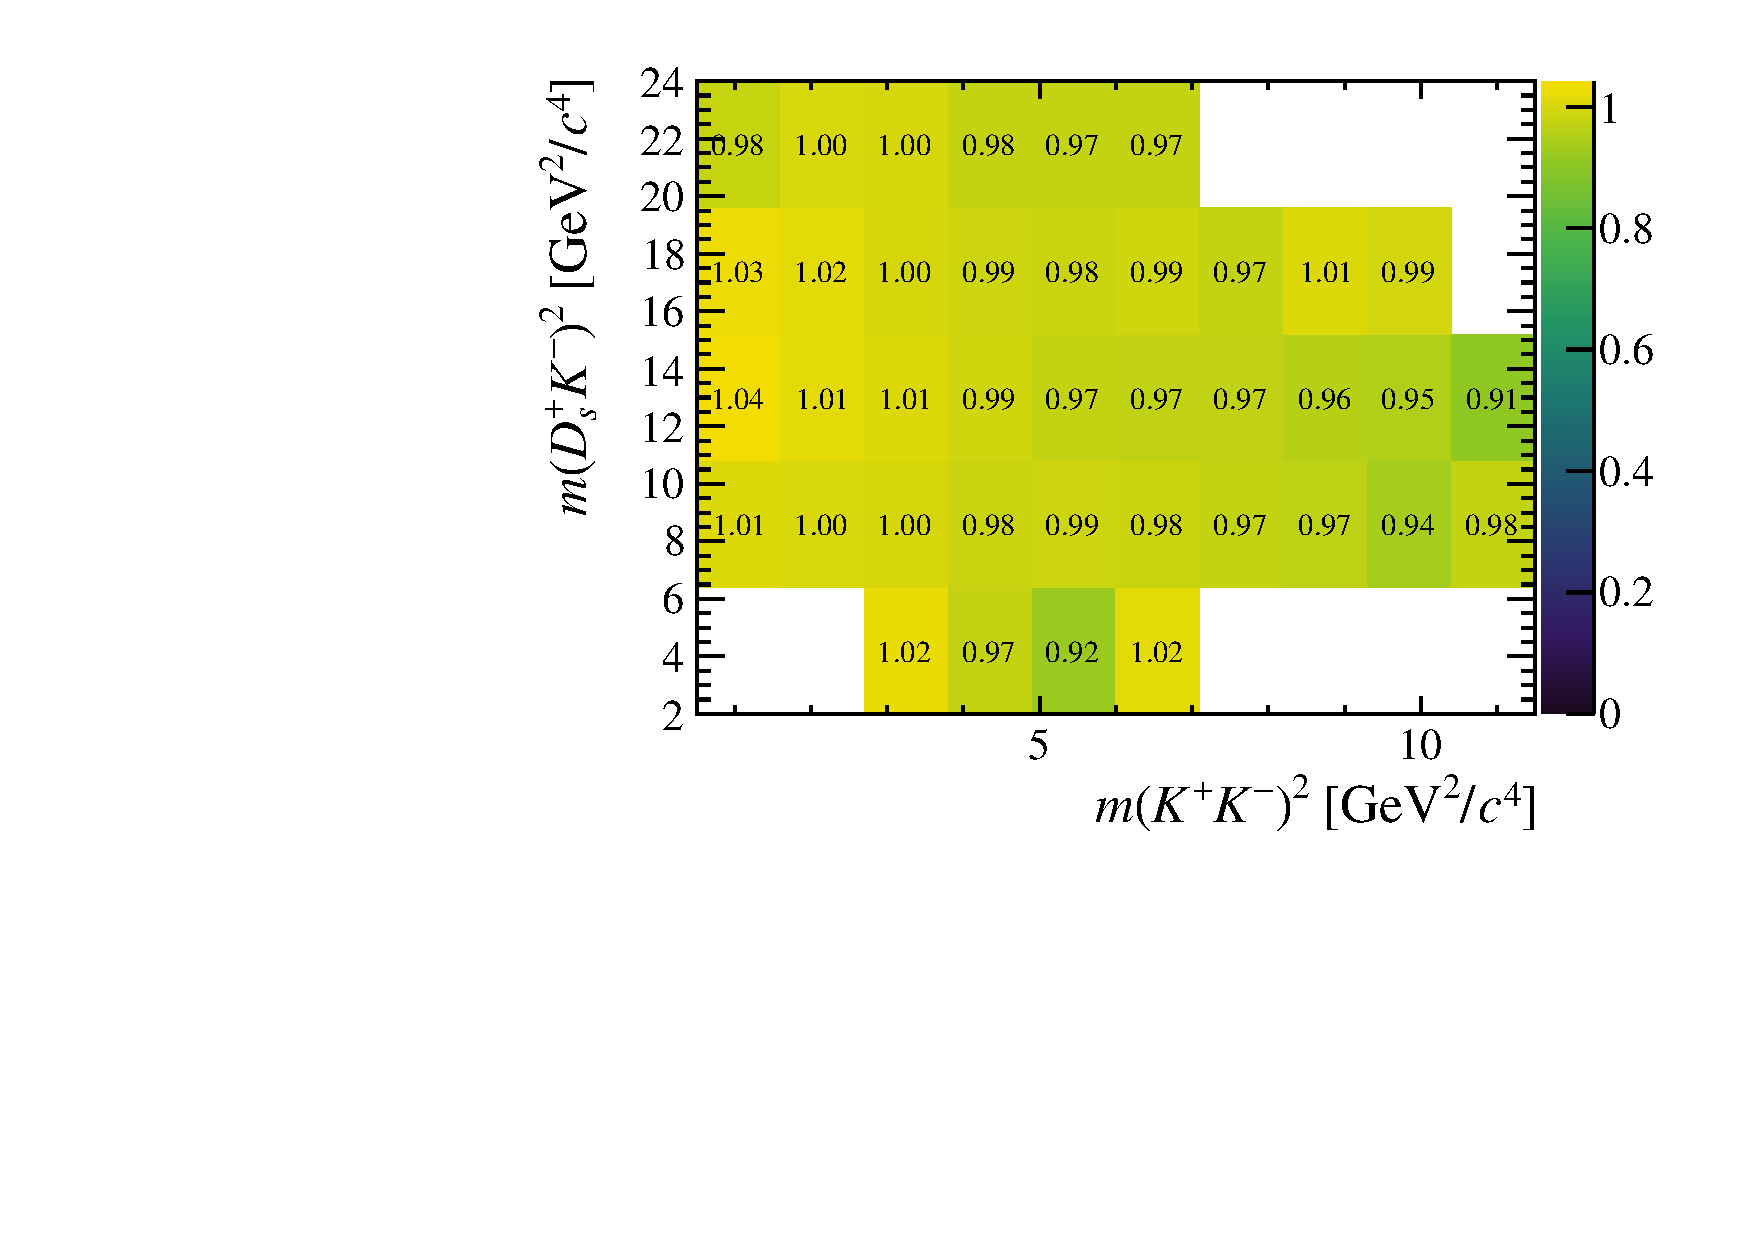
\includegraphics[width=1.0\textwidth]{figs/B2DsKK/Relative_Eff_PID_All.pdf}
      \caption{PID}
      \label{fig:B2DsKK_releff_PID}
   \end{subfigure}
   \begin{subfigure}[t]{0.4\textwidth}
      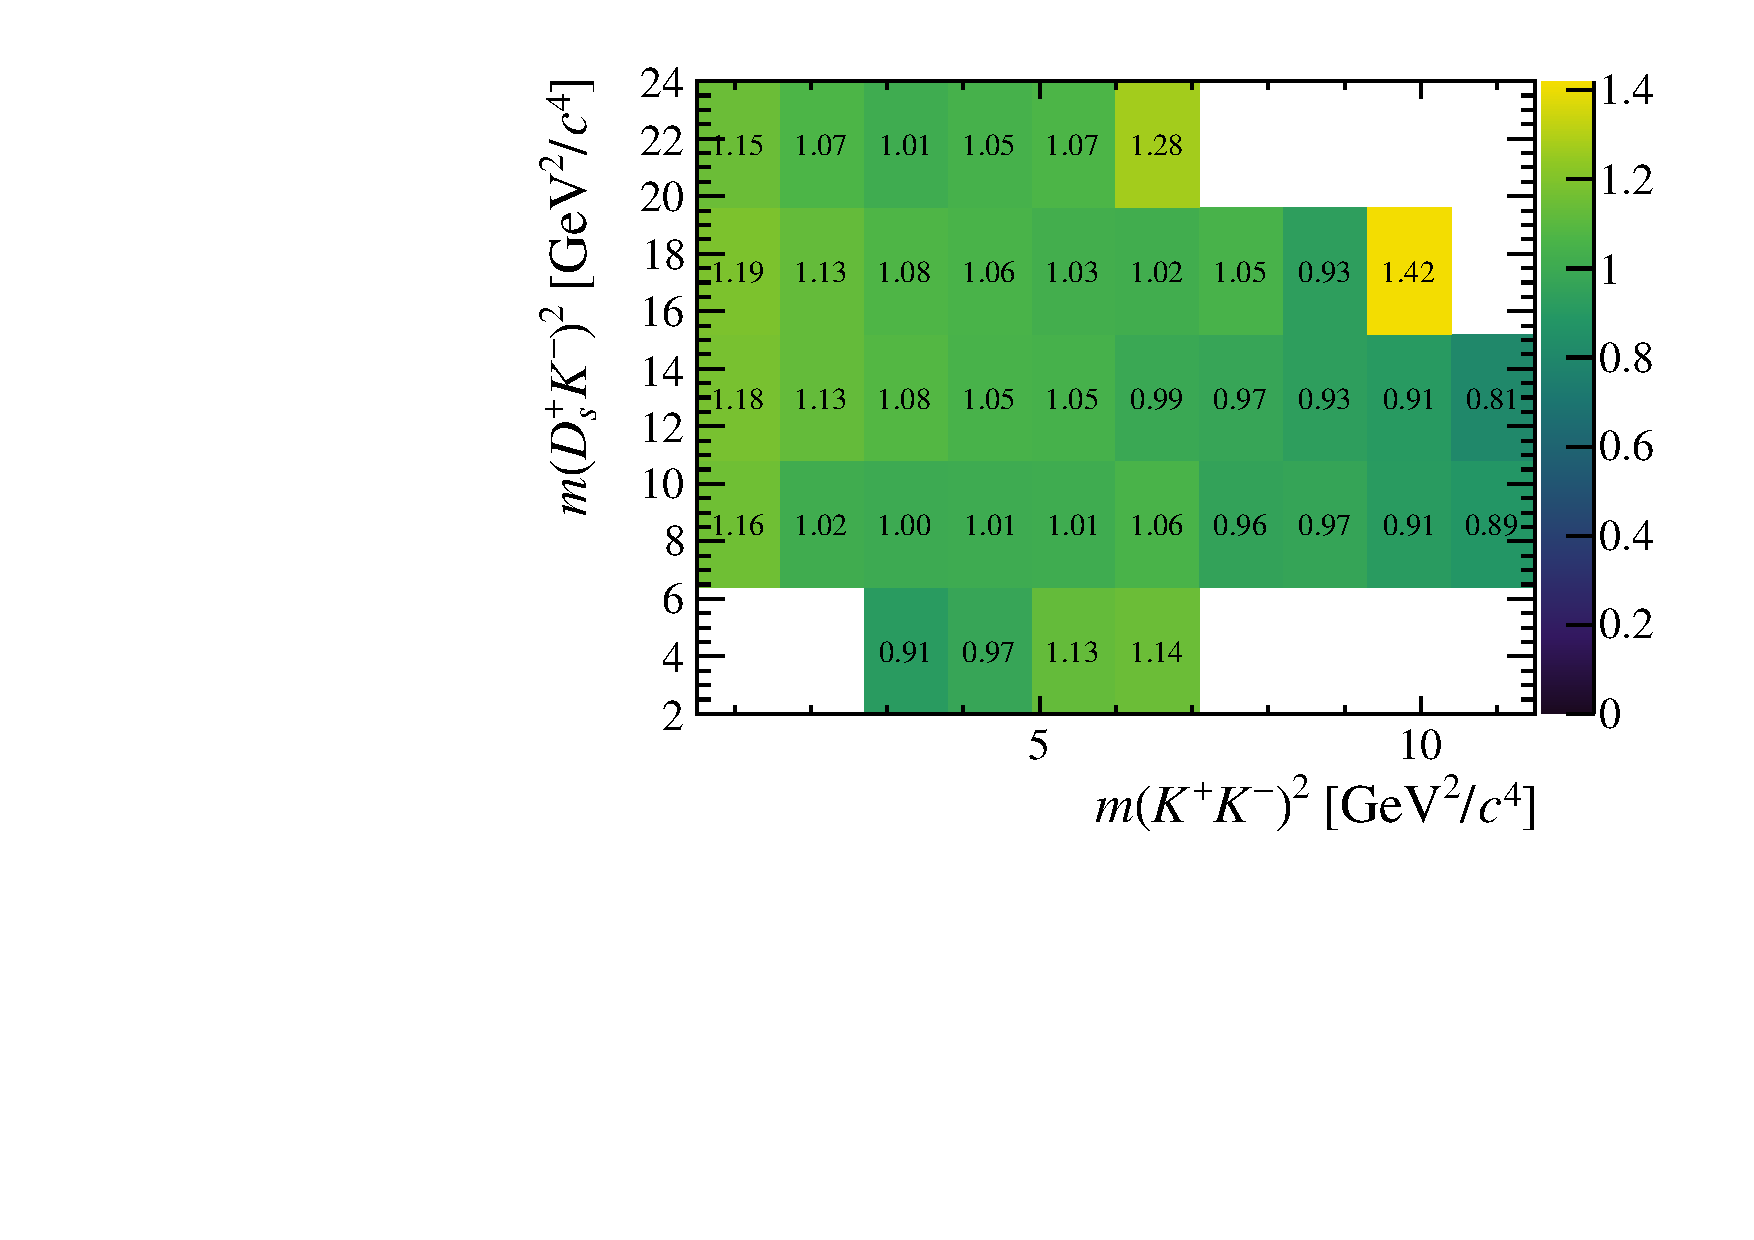
\includegraphics[width=1.0\textwidth]{figs/B2DsKK/Relative_Eff_BDT_All.pdf}
      \caption{MVA}
      \label{fig:B2DsKK_releff_MVA}
   \end{subfigure}
   \caption{Efficiencies}
   \label{fig:B2DsKK_dalitz_eff_three}
\end{figure}
%%%%%%%%%%%%%%%%%%%%%%%%%%%%%%%%%%%%%%%%%%%%%%%%%%%%%%%%%%


\subsubsection{MVA efficiency}

The MVA efficiency is determined from samples for signal and normalisation simulations in which the PID distributions have been corrected as described previously. This is different to the approach used in the search for \decay{\Bp}{\Dsp\phiz} decays (Sec.~\ref{sec:B2DsPhi_eff_MVA}) and is required to account for the variation in the efficiency across the phase-space. The corrected ProbNNx PID variables are used to determine the \Dsp and \phiz MVA classifiers and the efficiency of the MVA requirements determined in different positions in the Dalitz plot as shown in Fig.\ref{fig:B2DsKK_releff_MVA}. There is a strong dependence on the position, with decays at low $m^{2}(\Kp\Km)$ values having a larger relative efficiency than those at higher values. This is likely to be because the MVA methods were trained using a sample of \decay{\phiz}{\Kp\Km} decays, so the selection favourably selects candidates with an invariant mass near the \phiz meson mass. A cross check is performed to compare the MVA efficiencies determined directly using the classifier produced with the corrected PID variables and the method described in Sec.~\ref{sec:selection_MVA_eff} that uses the MVA training samples to calculate the efficiency. The values of the efficiency determined for each mode are compared in Fig.~\ref{fig:B2DsKK_PID_eff_crosscheck} as a function of the $m(\Kp\Km)$ mass. The MVA training modes only exist for two discreet values; $m(\Kp\Km)=m(\phiz)$ and $m(\Kp\Km)=m(\Dzb)$ represented by the red points. These are compared to the \decay{\Bp}{\Dsp\Kp\Km} and \decay{\Bp}{\Ds\Dzb} efficiencies from the corrected simulations in black and blue respectively. A good agreement is found.

%%%%%%%%%%%%%%%%%%%%%%%%%%%%%%%%%%%%%%%%%%%%%%%%%%%%%%%%%%
\begin{figure}[!h]
   \centering
   \begin{subfigure}[t]{0.4\textwidth}
      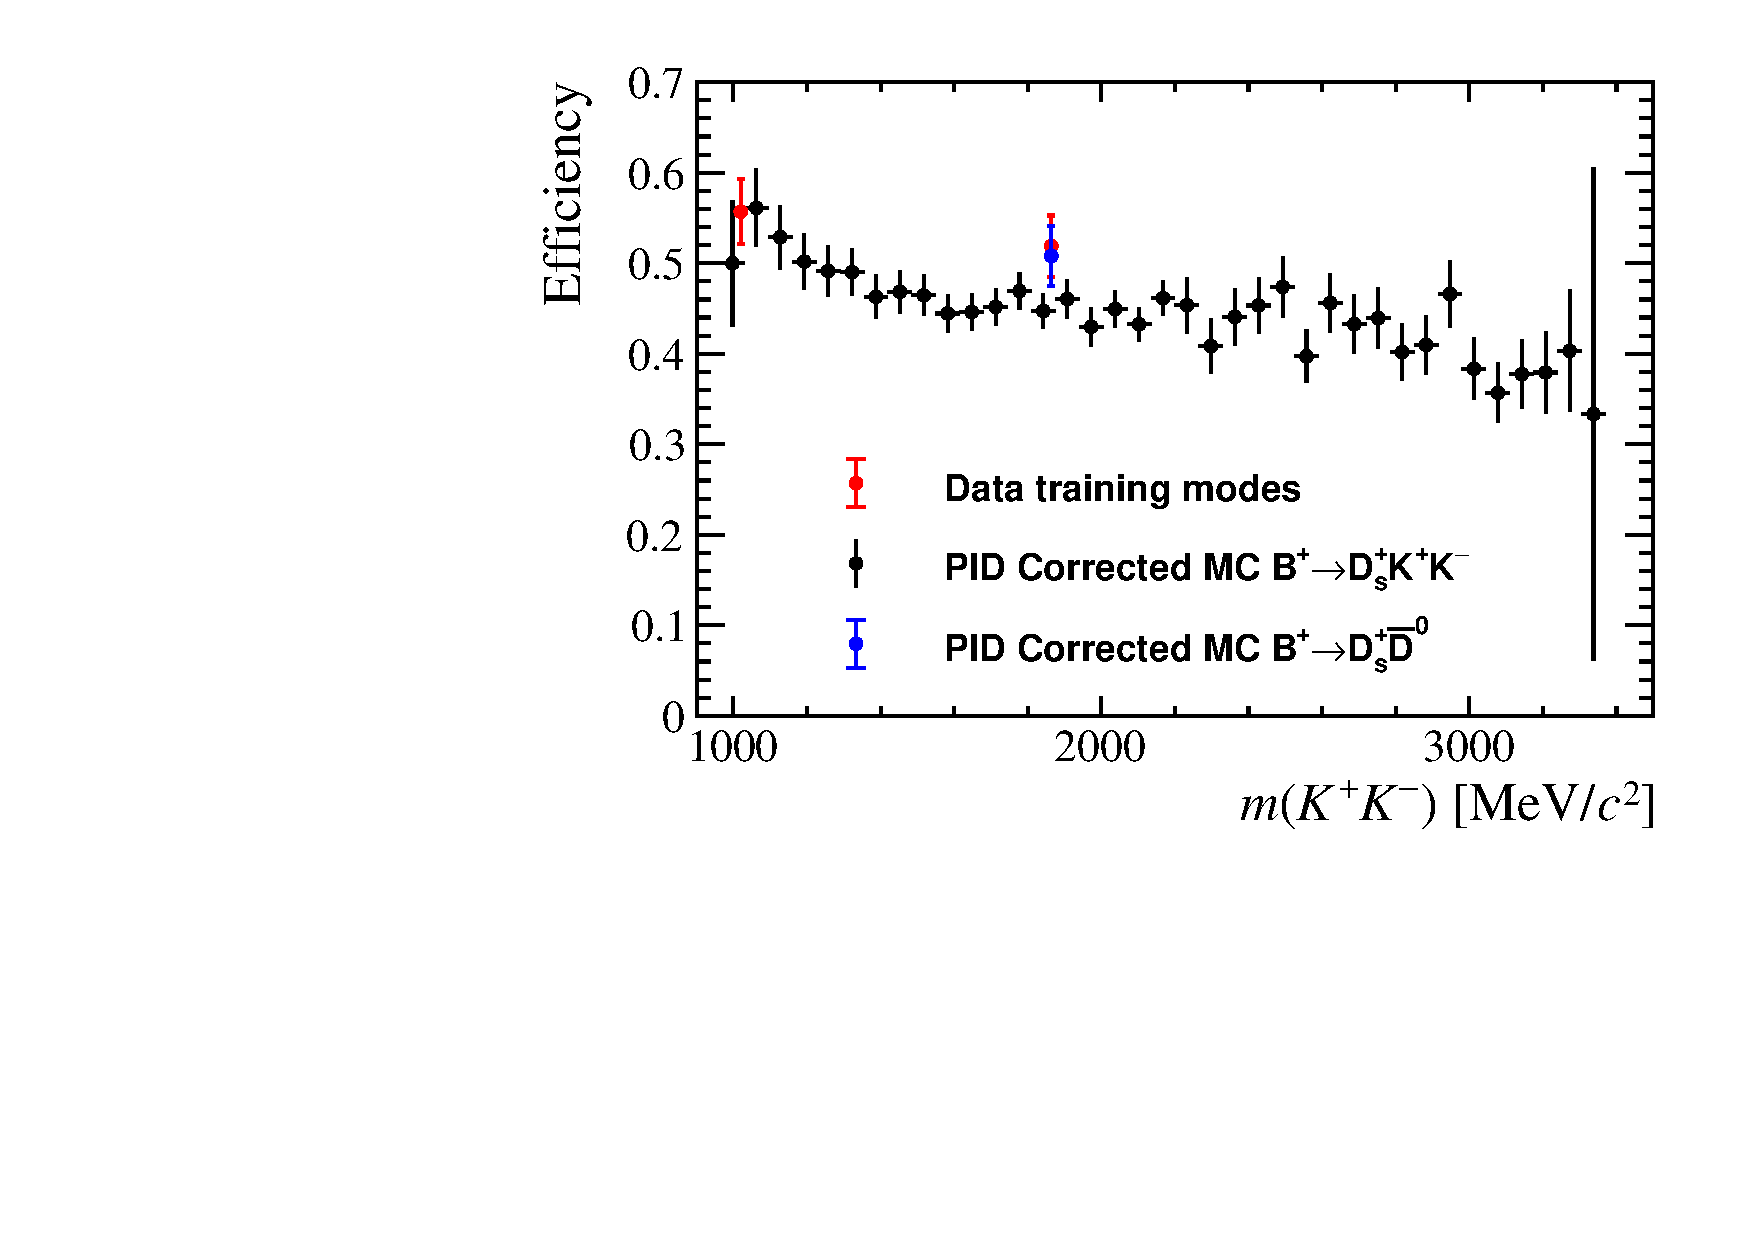
\includegraphics[width=1.0\textwidth]{figs/B2DsKK/mKK_eff_2011_Both.pdf}
      \caption{2011}
   \end{subfigure}
   \begin{subfigure}[t]{0.4\textwidth}
      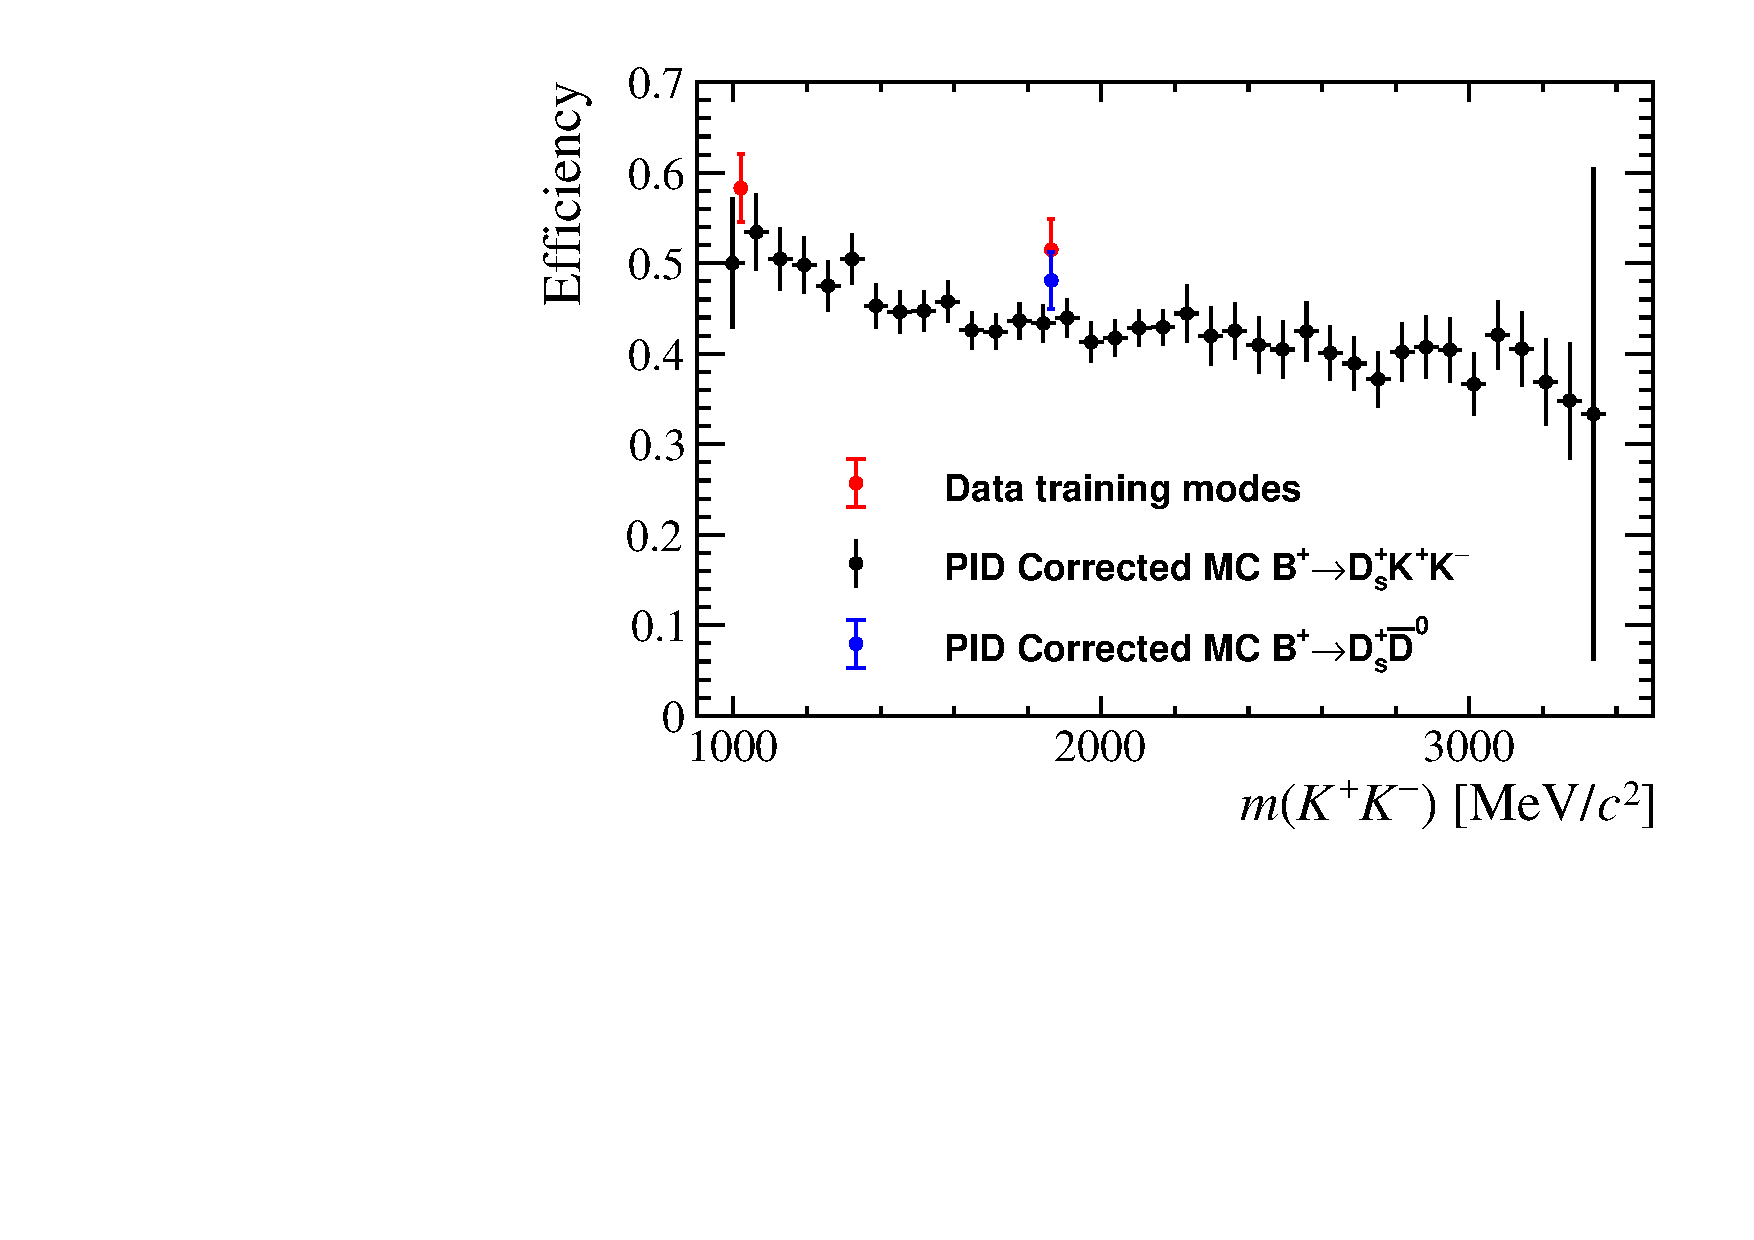
\includegraphics[width=1.0\textwidth]{figs/B2DsKK/mKK_eff_2012_Both.pdf}
      \caption{2012}
   \end{subfigure}
   \caption{The PID efficiency variation as a function $m(\Kp\Km)$ as determined from the MVA training modes (red) and the \decay{\Bp}{\Dsp\Kp\Km} and \decay{\Bp}{\Ds\Dzb} simulation samples (black and blue respectively). A good agreement is found between the red and black point at $m(\Kp\Km)=m(\phiz)$, and the red and blue point at $m(\Kp\Km)=m(\Dzb)$.}
   \label{fig:B2DsKK_PID_eff_crosscheck}
\end{figure}
%%%%%%%%%%%%%%%%%%%%%%%%%%%%%%%%%%%%%%%%%%%%%%%%%%%%%%%%%%

\section{Systematic uncertainties}
\label{sec:B2DsKK_systuncertainy}


A number of sources of systematic uncertainty are considered when determining the branching fraction for \decay{\Bp}{\Dsp\Kp\Km} decays.


\subsection{Relative efficiencies}
\label{sec:B2DsKK_sys_releff}



\subsection{Signal and normalisation PDFs}

Some parameters in the signal and normalisation PDFs are fixed to values obtained from simulation. These include the tail parameters, relative widths, and fractional amounts of the two CB functions that make up the PDFs. The values obtained from simulation have associated uncertainties arising from the limited simulation sample sizes. The nominal fits are repeated with the fixed parameters modified to values sampled from Gaussian distributions, with a width given by the parameter uncertainties. All parameters are changed simultaneously. The resulting variation of $0.036\times 10^{-6}$ is assigned as the associated systematic uncertainty. 

\subsection{Background PDFs}

In the signal mode the PDFs for the partially reconstructed background modes are taken directly from simulated events using one-dimensional kernel estimations~\cite{Cranmer:2000du}. In the nominal fit, these are smeared to account for the differences in the mass resolution between data and simulation. To account for any systematic uncertainty arising from the choice of resolution difference, the fit is repeated, randomly varying the smearing resolution each time. The resulting variation in the branching fraction is assigned as a systematic uncertainty. 

In the normalisation mode a number of choices are made about the partially reconstructed backgrounds, namely the kinematic limits of the \decay{\Bp}{\Dssp\Dzb} and \decay{\Bp}{\Dsp\Dstarzb}, and the external branching fractions of \decay{\Dssp}{\Dsp[\Pgamma/\piz]},
 \decay{\Dstarzb}{\Dzb[\Pgamma/\piz]} decays. These assumptions are simultaneously varied within the relevant uncertainties, resulting in a change of $0.015\times10^{-6}$ in the branching fraction.




\subsection{Charmless contribution}


{\color{Blue}
\begin{description}
\item \textbf{Signal PDF shapes}

\item \textbf{Background PDF shapes}

\item \textbf{Charmless Contribution} The expected charmless contribution is only a significant fraction of the measured yield for the normalisation mode, expected to be around 0.7\%. We assign this as the systematic uncertainty arising from the charmless contamination as this ratio would directly propagate to the branching fraction.

\item \textbf{BDT Efficiency Ratio} All of the sources of systematic uncertainty associated with the BDT efficiency ratio still apply here, particularly as the data trained efficiencies are still used to find the ratio in Run 2. 

An additional systematic is assigned to account for the use Run 1 Dalitz plot dependences on the BDT and PID ratios. We assume the shapes of the Dalitz plot dependences are the same for Run 1 and Run 2, but adjust the overall scale to match the efficiencies determined previously. However by looking at the differences between the efficiencies for $\B \to \Ds \Dz$ and $\B \to \Ds \phi$ in Table~\ref{tab:BDT}, one sees that the differences get larger in Run 2, implying the shape may indeed get steeper. As a very conservative estimate we take the largest difference between $\B \to \Ds \Dz$ and $\B \to \Ds \phi$ in Run 2 and subtract the smallest difference in Run 1. This gives a difference of 4.4\% which we assign as the systematic uncertainty. This is likely to be an overestimate of the effect on the final branching fraction as most of the signal events are found in a small area of the phase space, leading to smaller variations in efficiency. This systematic can be removed if support for Run 2 in \texttt{Meerkat}/\texttt{PIDCorr} becomes available before publishing.


\item \textbf{PID Efficiency Ratio} We assume the same systematic uncertainty for the ratio of PID efficiencies as previously discussed: 2\%. 

\item \textbf{Veto Efficiency Ratio} We assume the same systematic uncertainty for the ratio of PID efficiencies as previously discussed: 1.4\%. 


\item \textbf{MC Statistics} We use a larger sample of $\B \to \Ds K K$ MC than previously but the size of the normalisation mode MC sample has not increased, therefore we maintain the 2\% systematic for MC statistics.

\end{description}
}
%\subsection{Total Systematic Uncertainty}

\begin{table}[!ht]
\begin{center}
\begin{tabular}{  l   c   c }

\hline
\multirow{ 2}{*}{\textbf{Source of Uncertainty} }&\multicolumn{2}{ c }{ Systematic Uncertainty}           \\
                                                 &\textbf{Relative} & \textbf{Absolute ($\times 10^{-6}$)}\\
\hline 
BDT Relative Efficiency                     & 6.2\% & $0.44$\\
Using Run 1 shapes as Run 2                 & 4.4\% & $0.31$\\
MC statistics                               & 2.0\% & $0.14$\\
PID Relative Efficiency                     & 2.0\% & $0.14$\\
Veto Relative Efficiency                    & 1.4\% & $0.10$\\
Charmless Contribution                      & 0.7\% & $0.05$\\
Signal PDF parametrisation                  &-      & $0.036$  \\
Background PDF parametrisation              &-      & $0.015$  \\
\hline
Total                                       &       & $0.59$\\
\hline
Normalisation                               &       & $0.70$\\
\hline
\end{tabular}
\caption{Contributions to the total systematic uncertainty of the \decay{\Bp}{\Dsp\Kp\Km} branching fraction measurement. }
\label{table:B2DsKK_systematics}
\end{center}
\end{table}  

\section{Results}
\label{sec:B2DsKK_results}

%%%%%%%%%%%%%%%%%%%%%%%%%%%%%%%
The fit to $\decay{\Bp}{\Dsp\Kp\Km}$ candidates finds a total yield of $N(\decay{\Bp}{\Dsp\Kp\Km}) = 443 \pm 29 $ candidates. 
This constitutes the first observation of this decay mode.
The branching fraction is calculated as
\begin{equation}
\mathcal{B}(\decay{\Bp}{\Dsp\Kp\Km}) = \frac{ N_{\text{corr}}(\decay{\Bp}{\Dsp\Kp\Km}) }{ N(\decay{\Bp}{\Dsp\Dzb}) } \times \mathcal{B}(\decay{\Bp}{\Dsp\Dzb}) \times \mathcal{B}(\decay{\Dzb}{\Kp\Km})
\label{eq:DsKKBranchingfraction}
\end{equation}
\noindent where $N(\decay{\Bp}{\Dsp\Dzb})$ is the yield of normalisation decays, and $N_{\text{corr}}(\decay{\Bp}{\Dsp\Kp\Km})$ is defined to be
\begin{equation}
N_{\text{corr}}(\decay{\Bp}{\Dsp\Kp\Km}) =  \sum\limits_{i} \frac{W_{i}}{\epsilon^{\text{ratio}}_{i}},
\end{equation}
\noindent where $W_{i}$ is the per-candidate weight, as determined by the \sPlot technique for candidate $i$; and $\epsilon^{\text{ratio}}_{i}$ represents the relative efficiency of the signal and normalisation modes $\epsilon_{i}(\decay{\Bp}{\Dsp\Kp\Km})/\epsilon(\decay{\Bp}{\Dsp\Dzb})$ in the relevant bin of the $\decay{\Bp}{\Dsp\Kp\Km}$ Dalitz plot. 


%The uncertainty of the corrected signal yield is calculated following the same procedure as outlined in the \decay{\Bp}{\Dp\Kp\pim} search analysis note~\cite{Wallace:2010891} and summarised here. 

The uncertainty on the corrected yield, $N_{\text{corr}}(\decay{\Bp}{\Dsp\Kp\Km})$, is in principle given by

\begin{equation}
\sigma(N_{\text{corr}}) =  \sqrt{\sum\limits_{i} \left(\frac{W_{i}}{\epsilon^{\text{ratio}}_{i}} \right)^{2}}.
\end{equation}
However, the fit used to determine the \sWeights only allows the yields to float, as opposed to the nominal fit that has additional floating parameters including the signal position and width. This means that this estimate of the corrected yield uncertainty could neglect the uncertainty due to the shape parameters: \ie the uncertainty calculated from the weights, $\sigma_{\text{yields only}}(N) = \sqrt{\sum{W_{i}^{2}}}$, can be less than the uncertainty returned by the nominal fit, $\sigma_{\text{fit}}(N)$.

To correctly account for this possibility, the uncertainty from the shape parameters is separated from the the total uncertainty: $\sigma_{\text{shape}}(N) = \sqrt{\sigma_{\text{fit}}(N)^{2}-\sigma_{\text{yields only}}(N)^{2}}$.
This extra uncertainty is then scaled by the corrected yield to give the total uncertainty


\begin{equation}
\sigma_{\text{corr}}(N_{\text{corr}}) =  \sqrt{  \sigma(N_{\text{corr}})^{2} +  \left( \frac{N_{\text{corr}}}{N} \sigma_{shape}(N) \right)^{2}}.
\end{equation}
For the nominal fit the uncertainties are summarised in Table~\ref{table:DsKK_fit_errors}.

\begin{table}[!ht]
\begin{center}
\begin{tabular}{  c | c   }
\hline
Uncertainty                             &  Value \\
\hline 
$\sigma(N_{\text{corr}})$               & 13.0\\
$\sigma_{\text{fit}}(N)$                & 29.4\\
$\sigma_{\text{yields only}}(N)$        & 25.4\\
$\sigma_{\text{shape}}(N)$              & 14.7 \\ 
\hline
$\sigma_{\text{corr}}(N_{\text{corr}})$ & 14.9 \\ 
\hline
\end{tabular}
\caption{The various uncertainties as detailed in Section~\ref{sec:B2DsKK_results} and their values in the nominal fit.}
\label{table:DsKK_fit_errors}
\end{center}
\end{table}

The corrected yield ratio can be expressed as the ratio of signal and normalisation branching fractions using Eq.~\ref{eq:DsKKBranchingfraction}. The value is measured to be 
\begin{equation}
\frac{ N_{\text{corr}}(\decay{\Bp}{\Dsp\Kp\Km}) }{ N(\decay{\Bp}{\Dsp\Dzb}) } = \frac{\mathcal{B}(\decay{\Bp}{\Dsp\Kp\Km})}{\mathcal{B}(\decay{\Bp}{\Dsp\Dzb})\mathcal{B}(\decay{\Dzb}{\Kp\Km})}  = 0.197 \pm 0.015 \pm 0.017, 
\end{equation}
where the first uncertainty is statistical, and the second is systematic.

The branching fraction for $\decay{\Bp}{\Dsp\Kp\Km}$ decays is determined to be 

\begin{equation}
\mathcal{B}(\decay{\Bp}{\Dsp\Kp\Km}) = (7.1 \pm 0.5 \pm 0.6 \pm 0.7) \times 10^{-6},
\end{equation}
where the first uncertainty is statistical, the second is systematic and the third from the branching fractions of $\decay{\Dzb}{\Kp\Km}$ and of the normalisation mode $\decay{\Bp}{\Dsp\Dzb}$. 
The values used for the branching fractions are $\mathcal{B}(\decay{\Dz}{\Kp\Km}) = (4.01 \pm 0.07)\times10^{-3}$ and $\mathcal{B}(\decay{\Bp}{\Dsp\Dzb}) = (9.0 \pm 0.9)\times10^{-3}$~\cite{PDG2016}. 
The two-body projections $m(D_{s}^{+}K^{-})$ and $m(K^{+}K^{-})$ are obtained for the signal component using the \sPlot technique, shown in Fig.~\ref{fig:B2DsKK_twobodyprojections}. No significant peak is observed in the \phiz region of the $m(\Kp\Km)$ plot; rather a broad distribution of candidates is found in the region up to $m(\Kp\Km) \simeq 1900 \mevcc$.

%%%%%%%%%%%%%%%%%%%%%%%%%%%%%%%%%%%%%%%%%%%%%%%%%%%%%%%%%%
\begin{figure}[!h]
    \centering
    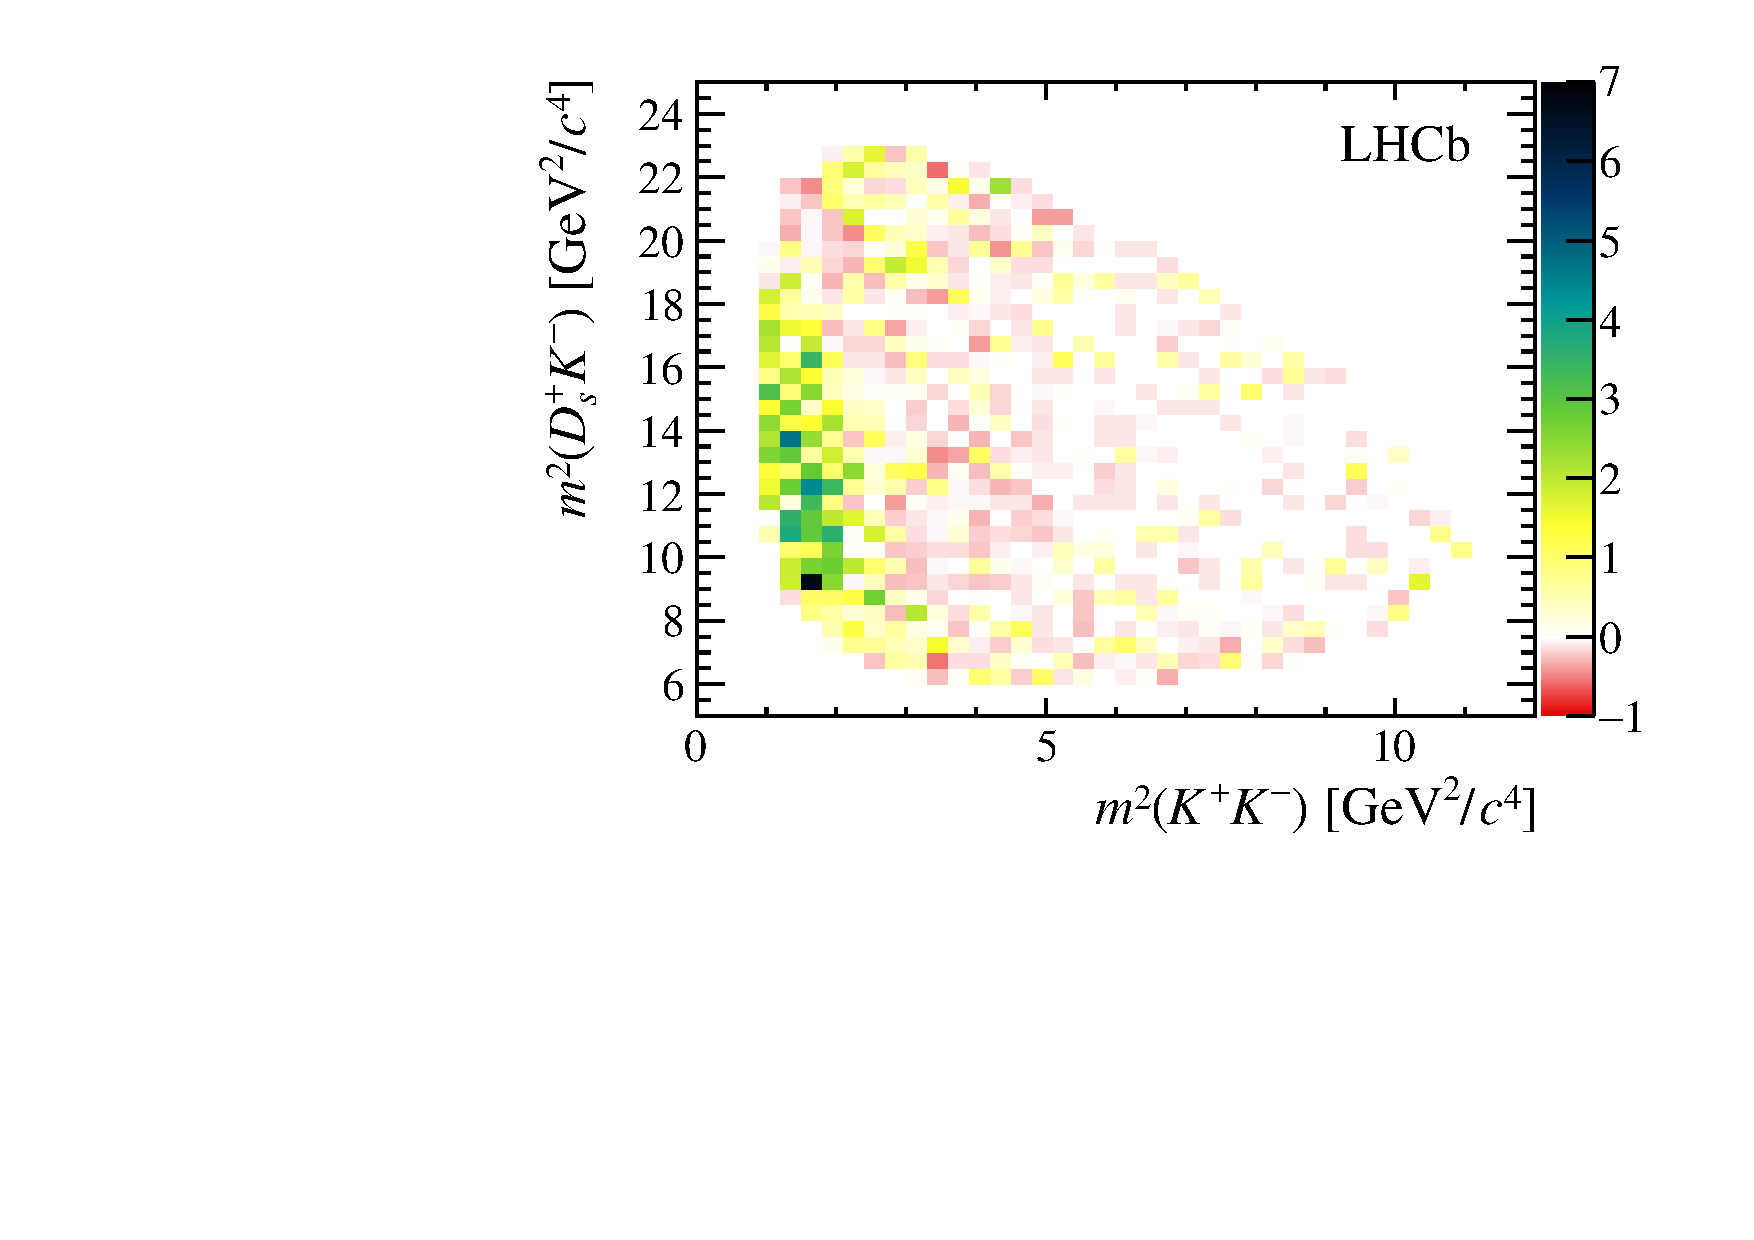
\includegraphics[width=0.8\textwidth]{figs/B2DsKK/Dalitz_plot_sweighted.pdf}
    \caption{Dalitz plot}
    \label{fig:B2DsKK_Dalitzplot}   
\end{figure}
%%%%%%%%%%%%%%%%%%%%%%%%%%%%%%%%%%%%%%%%%%%%%%%%%%%%%%%%%%

%%%%%%%%%%%%%%%%%%%%%%%%%%%%%%%%%%%%%%%%%%%%%%%%%%%%%%%%%%
\begin{figure}[!h]
    \centering
    \begin{subfigure}[t]{0.49\textwidth}
        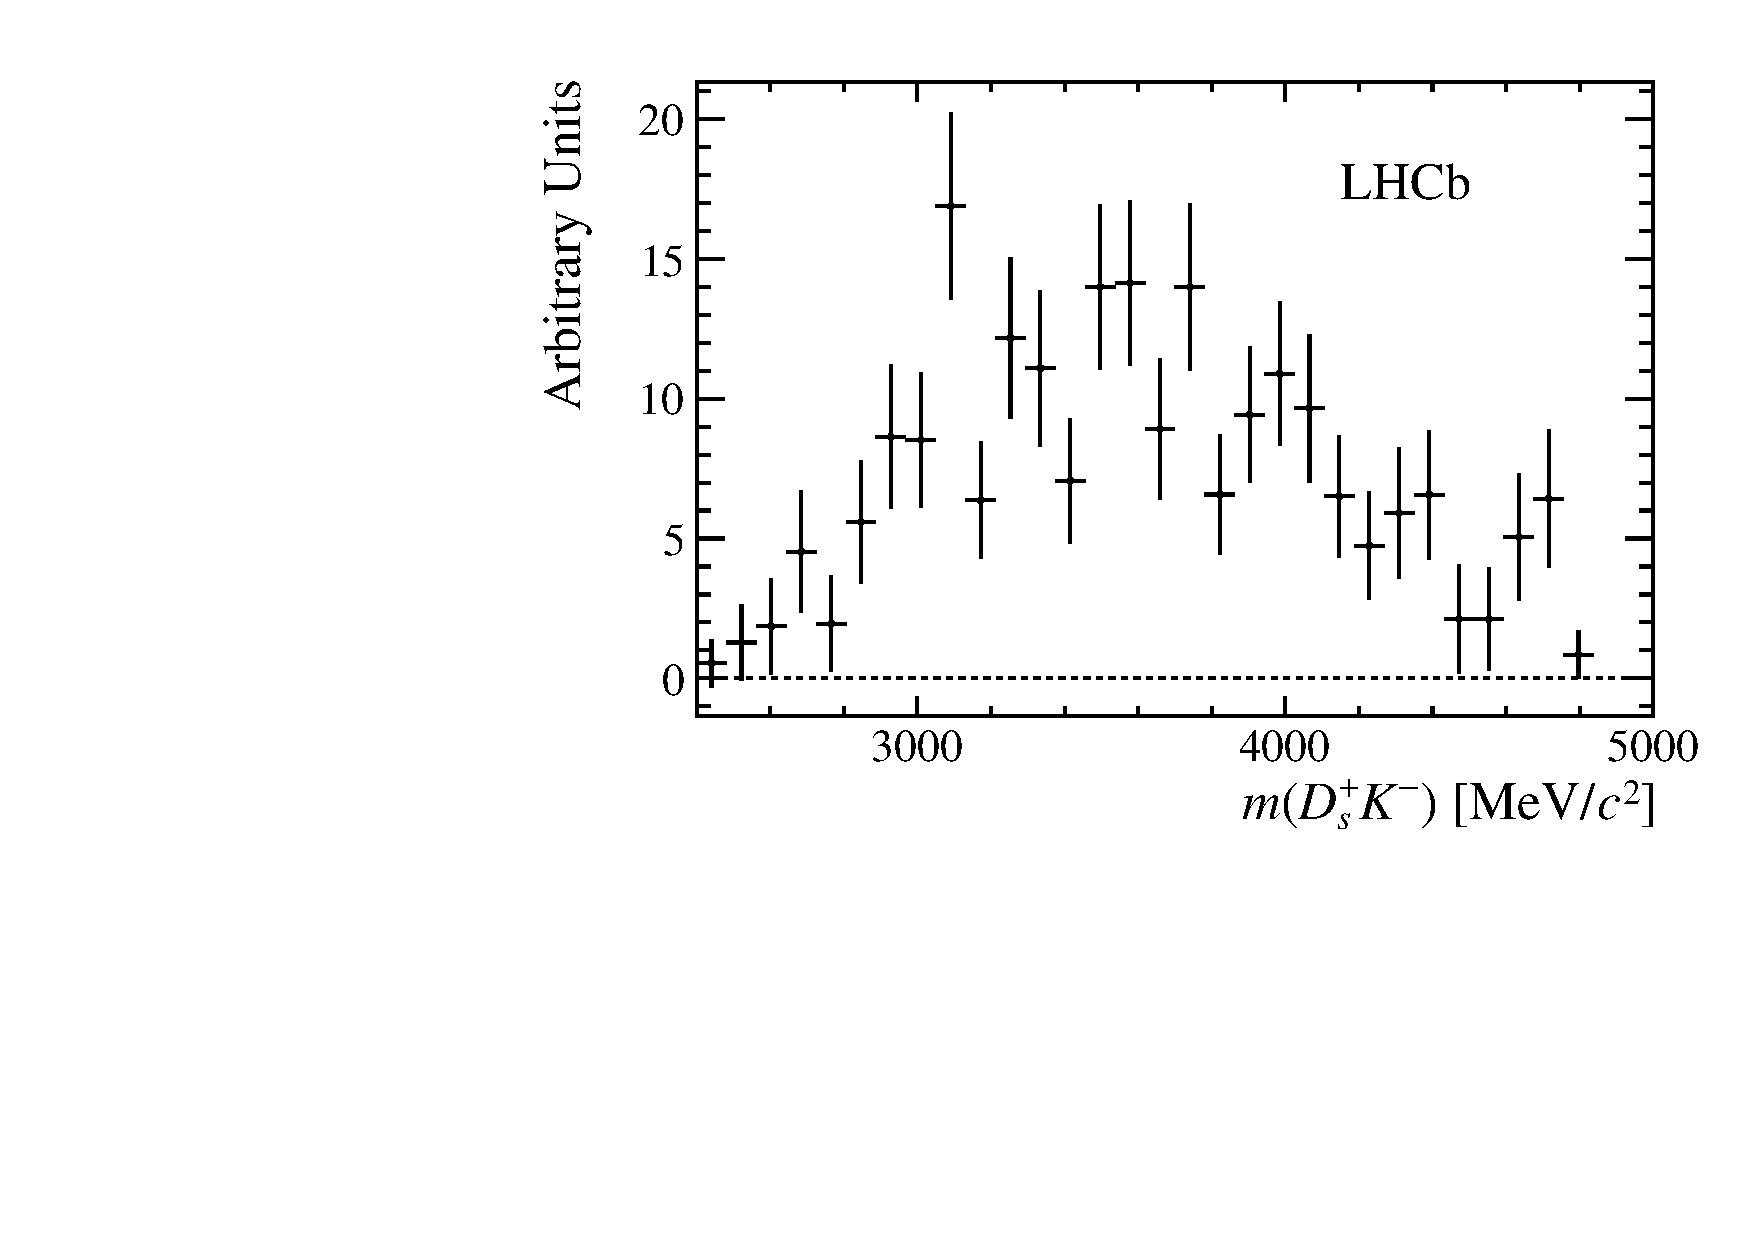
\includegraphics[width=1.0\textwidth]{figs/B2DsKK/DsKm_mass_sweighted.pdf}
        %\caption{Normalisation without selection}
    \end{subfigure}
    \begin{subfigure}[t]{0.49\textwidth}
        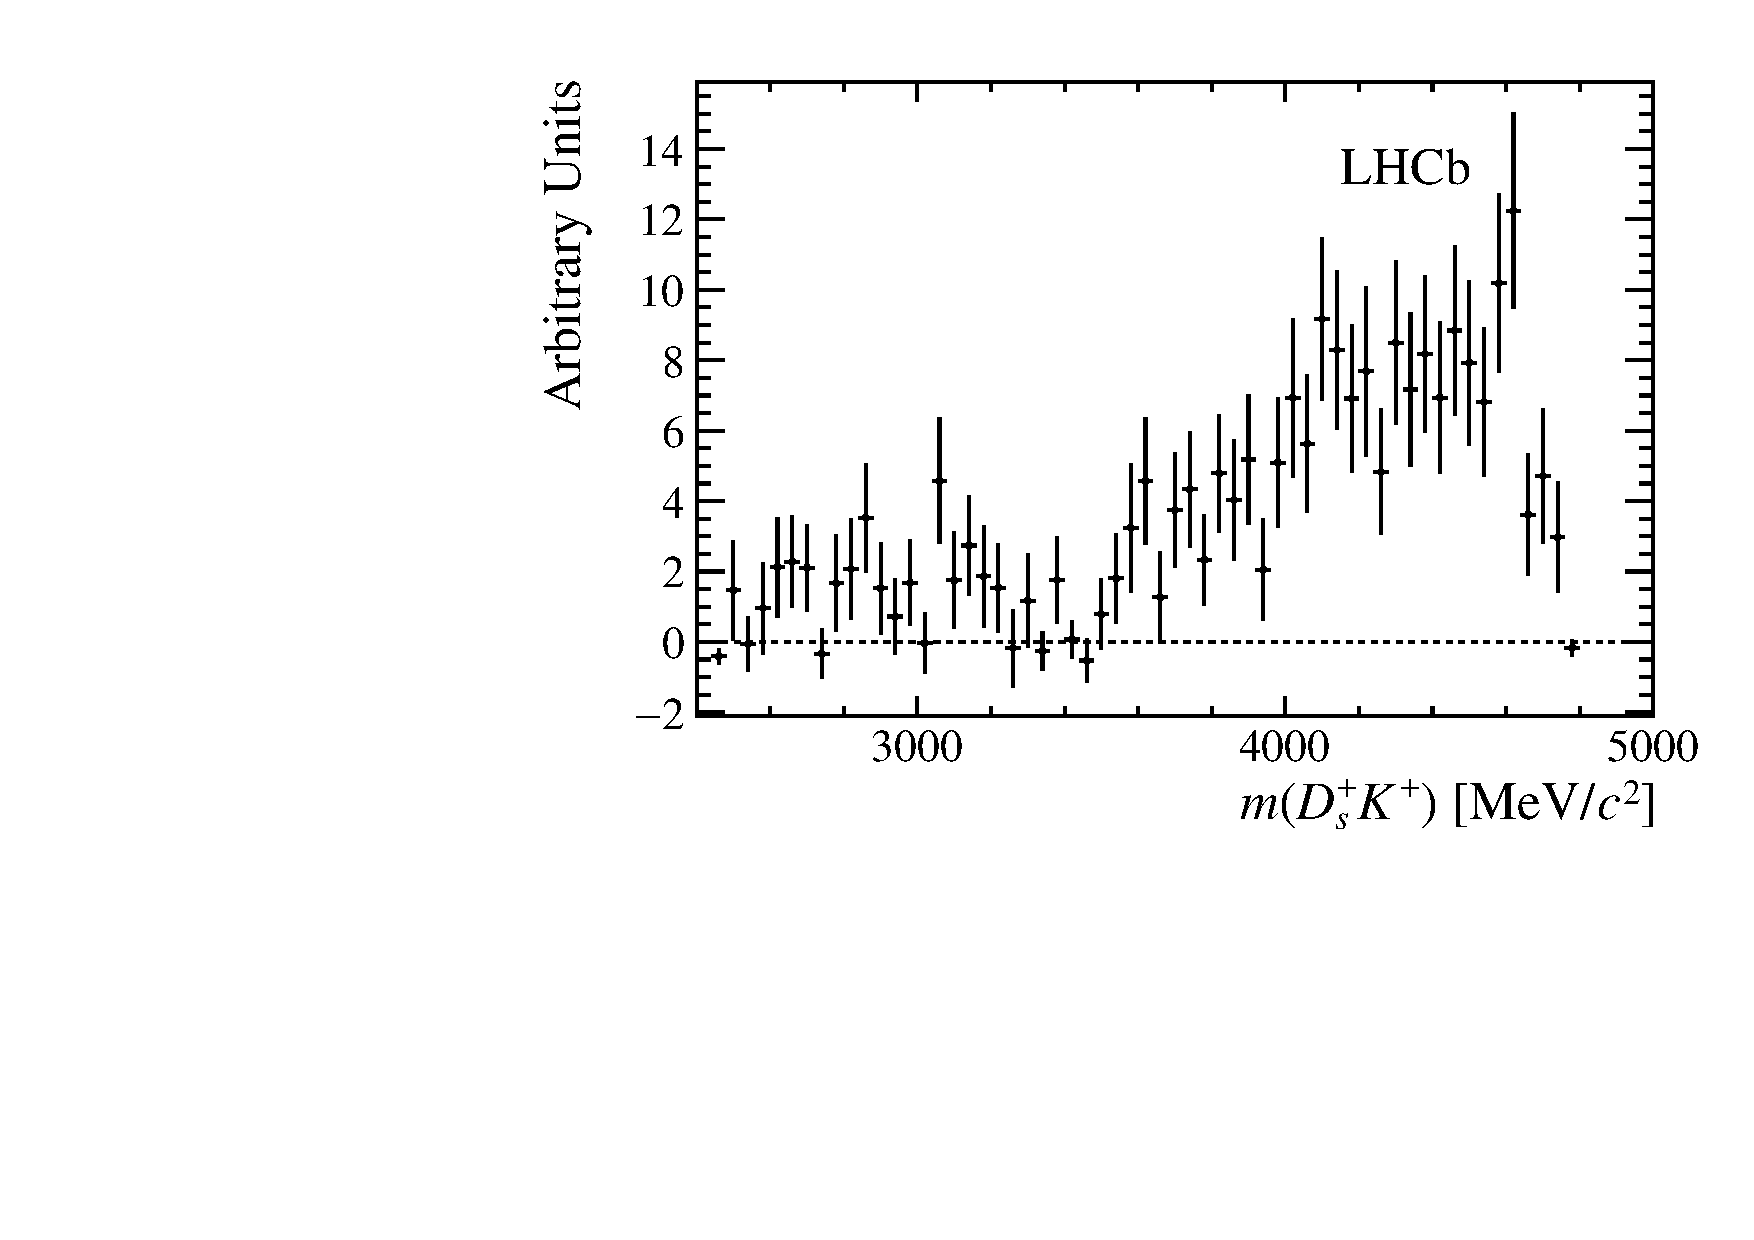
\includegraphics[width=1.0\textwidth]{figs/B2DsKK/DsKp_mass_sweighted.pdf}
        %\caption{Normalisation without selection}
    \end{subfigure}
    \begin{subfigure}[t]{0.49\textwidth}
        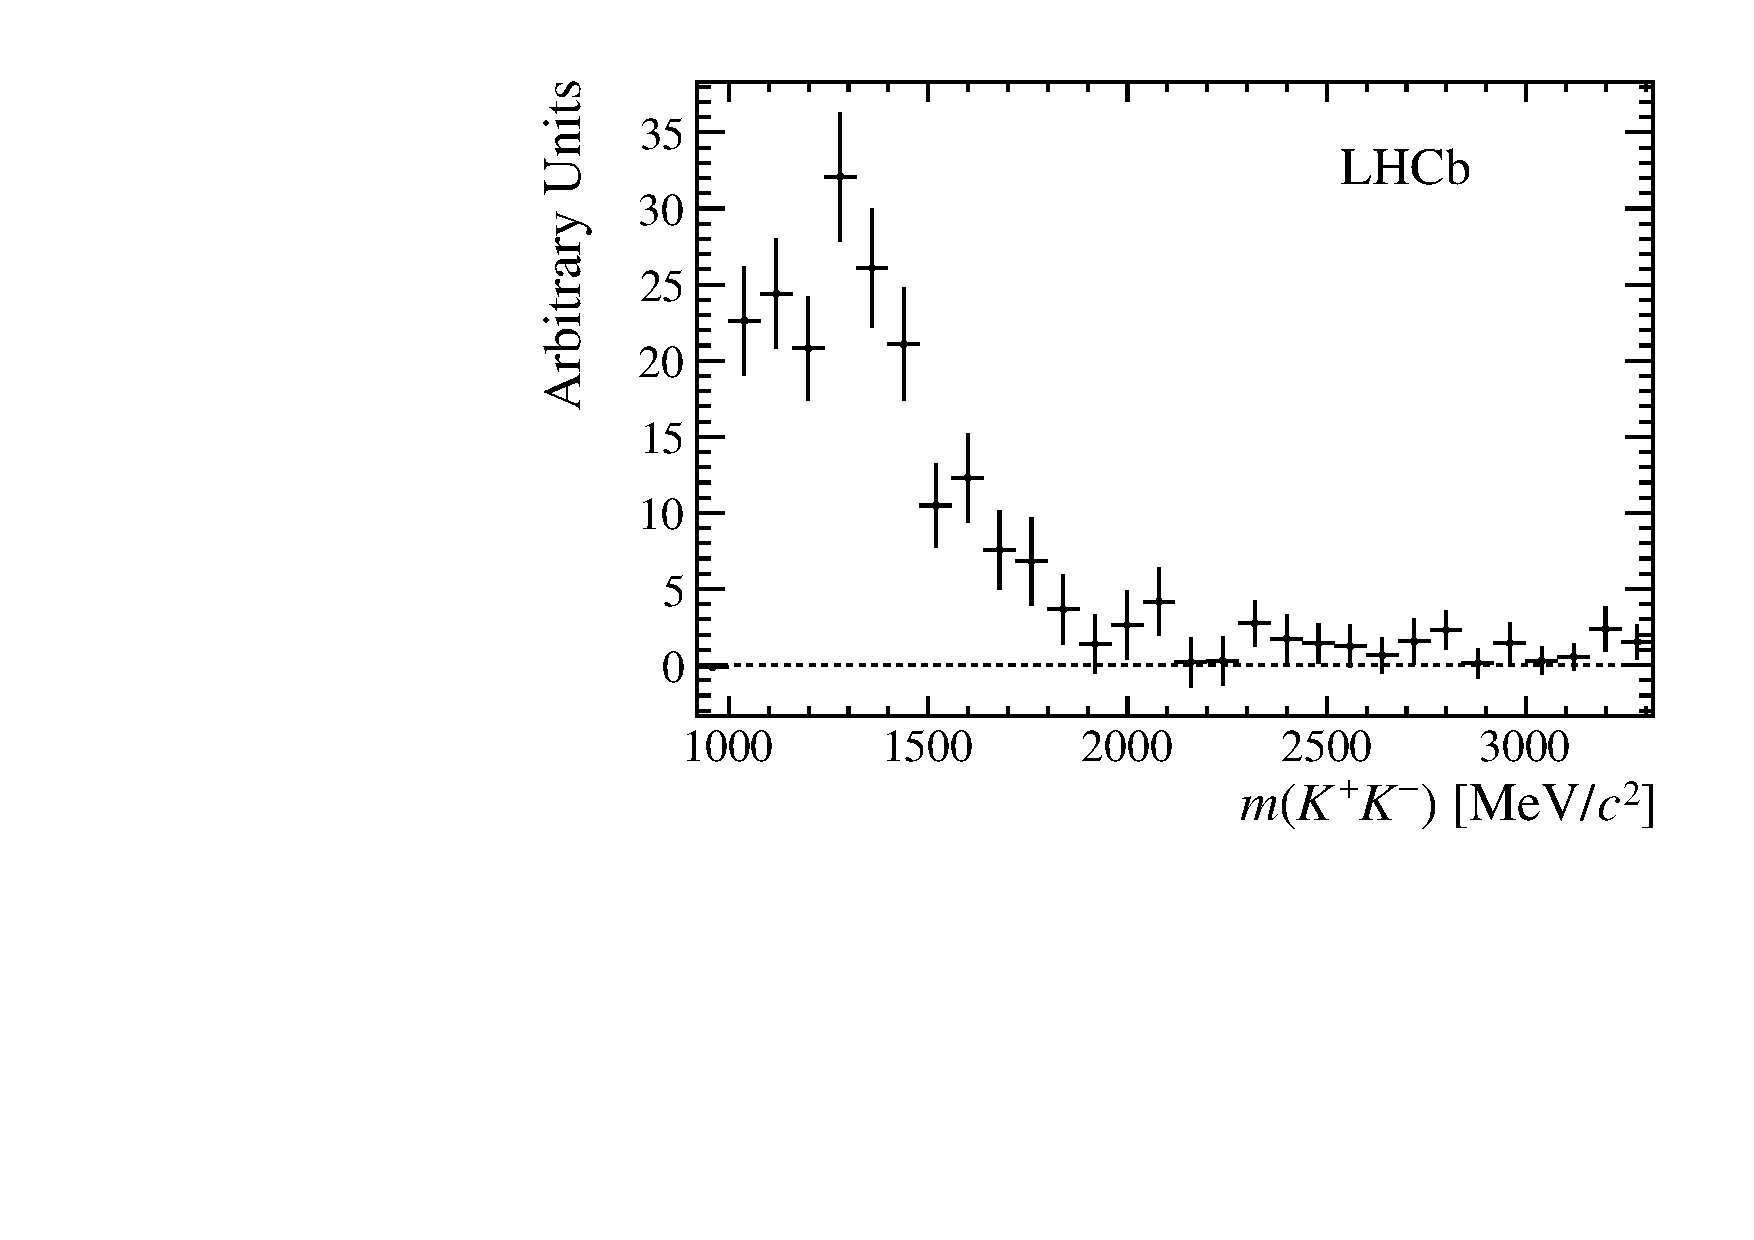
\includegraphics[width=1.0\textwidth]{figs/B2DsKK/phi_mass_sweighted.pdf}
        %\caption{Normalisation without selection}
    \end{subfigure}
    \caption{Two-body mass projections}
    \label{fig:B2DsKK_twobodyprojections}
\end{figure}
%%%%%%%%%%%%%%%%%%%%%%%%%%%%%%%%%%%%%%%%%%%%%%%%%%%%%%%%%%



%%%%%%%%%%%%%%%%%%%%%%%%%%%%%%%%%%%%%%%%%%%%%%%%%%%%%%%%%%
\begin{figure}[!h]
    \centering
    \begin{subfigure}[t]{0.59\textwidth}
        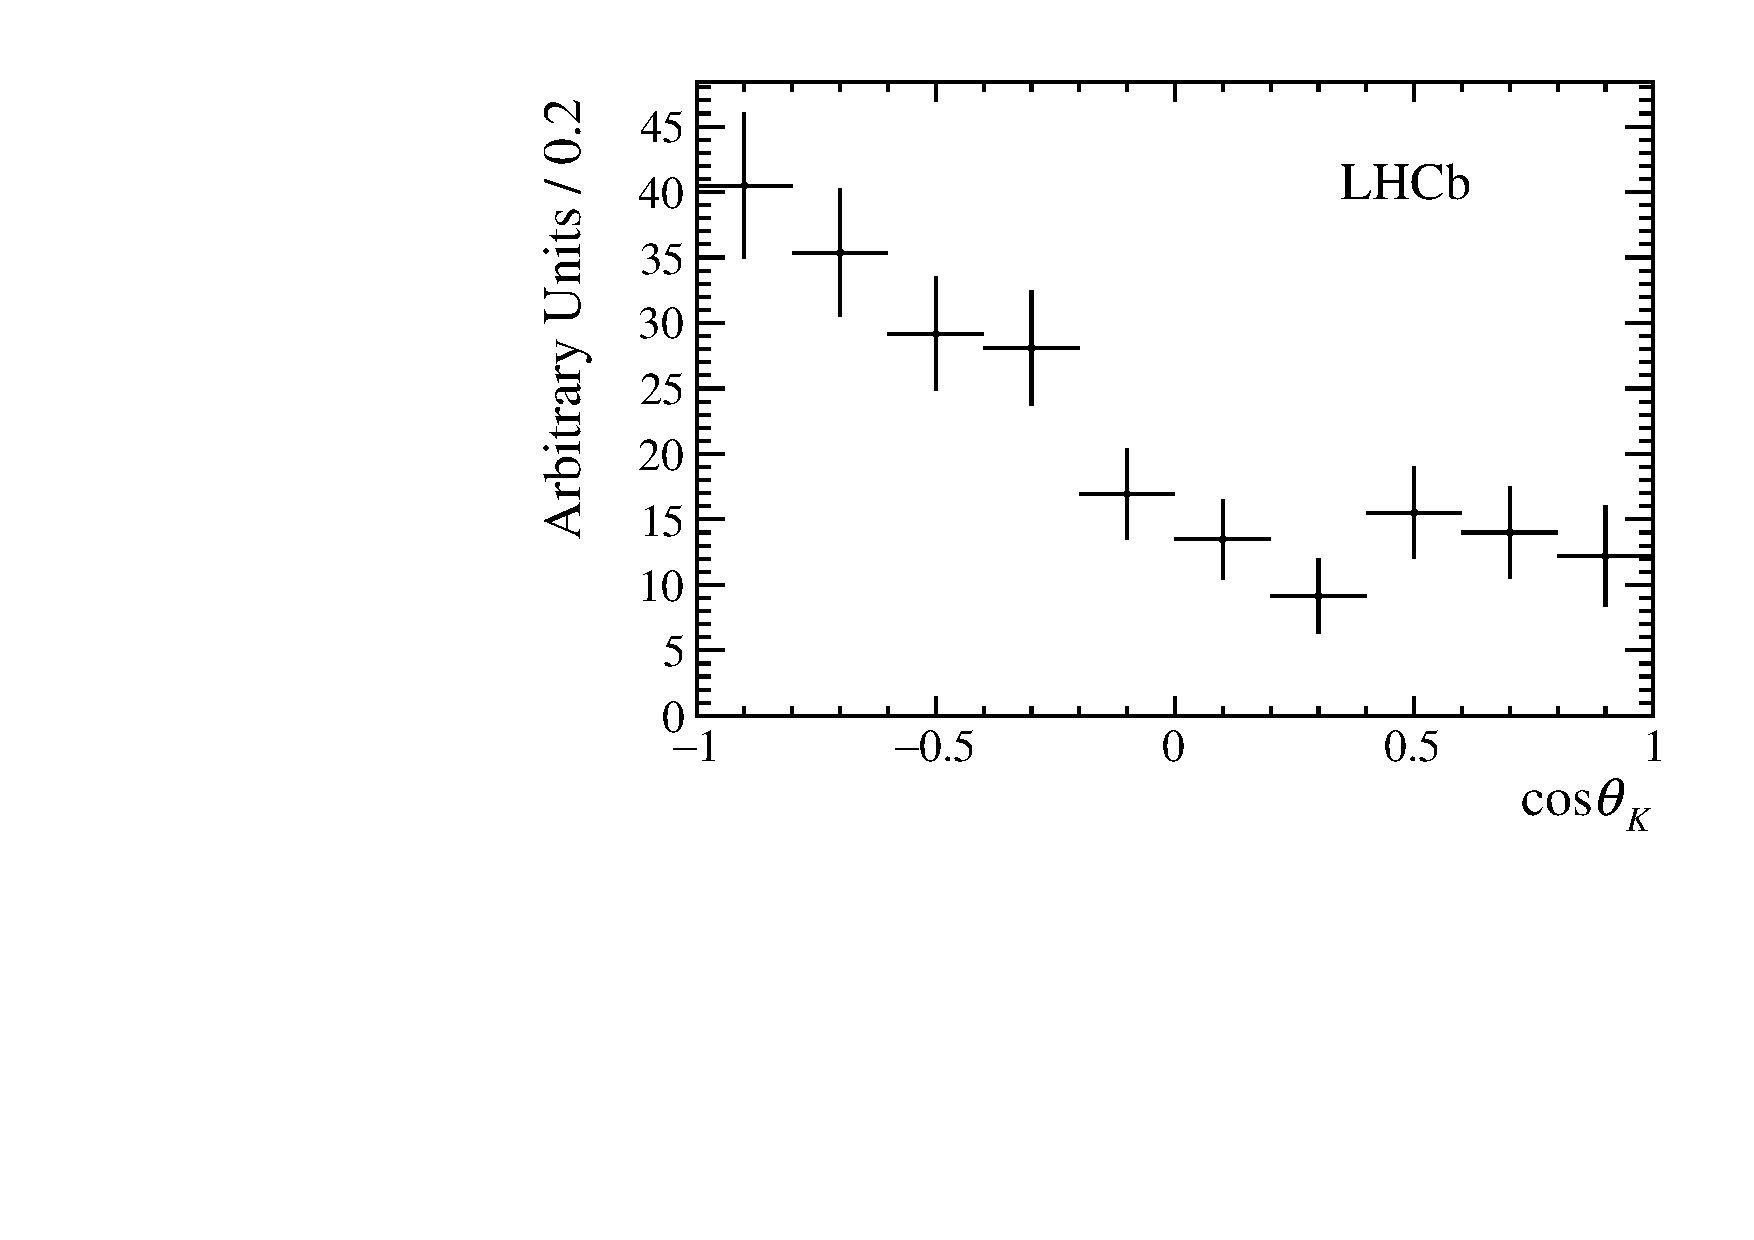
\includegraphics[width=1.0\textwidth]{figs/B2DsKK/helAngle_sweighted.pdf}
        %\caption{Normalisation without selection}
    \end{subfigure}
    \caption{Helicity angle}
    \label{fig:B2DsKK_twobodyprojections}
\end{figure}
%%%%%%%%%%%%%%%%%%%%%%%%%%%%%%%%%%%%%%%%%%%%%%%%%%%%%%%%%%



%%%%%%%%%%%%%%%%%%%%%%%%%%%%%%%%%%%%%%%%%%%%%%%%%%%%%%%%%%
\begin{figure}[!h]
    \centering
    \begin{subfigure}[t]{0.49\textwidth}
        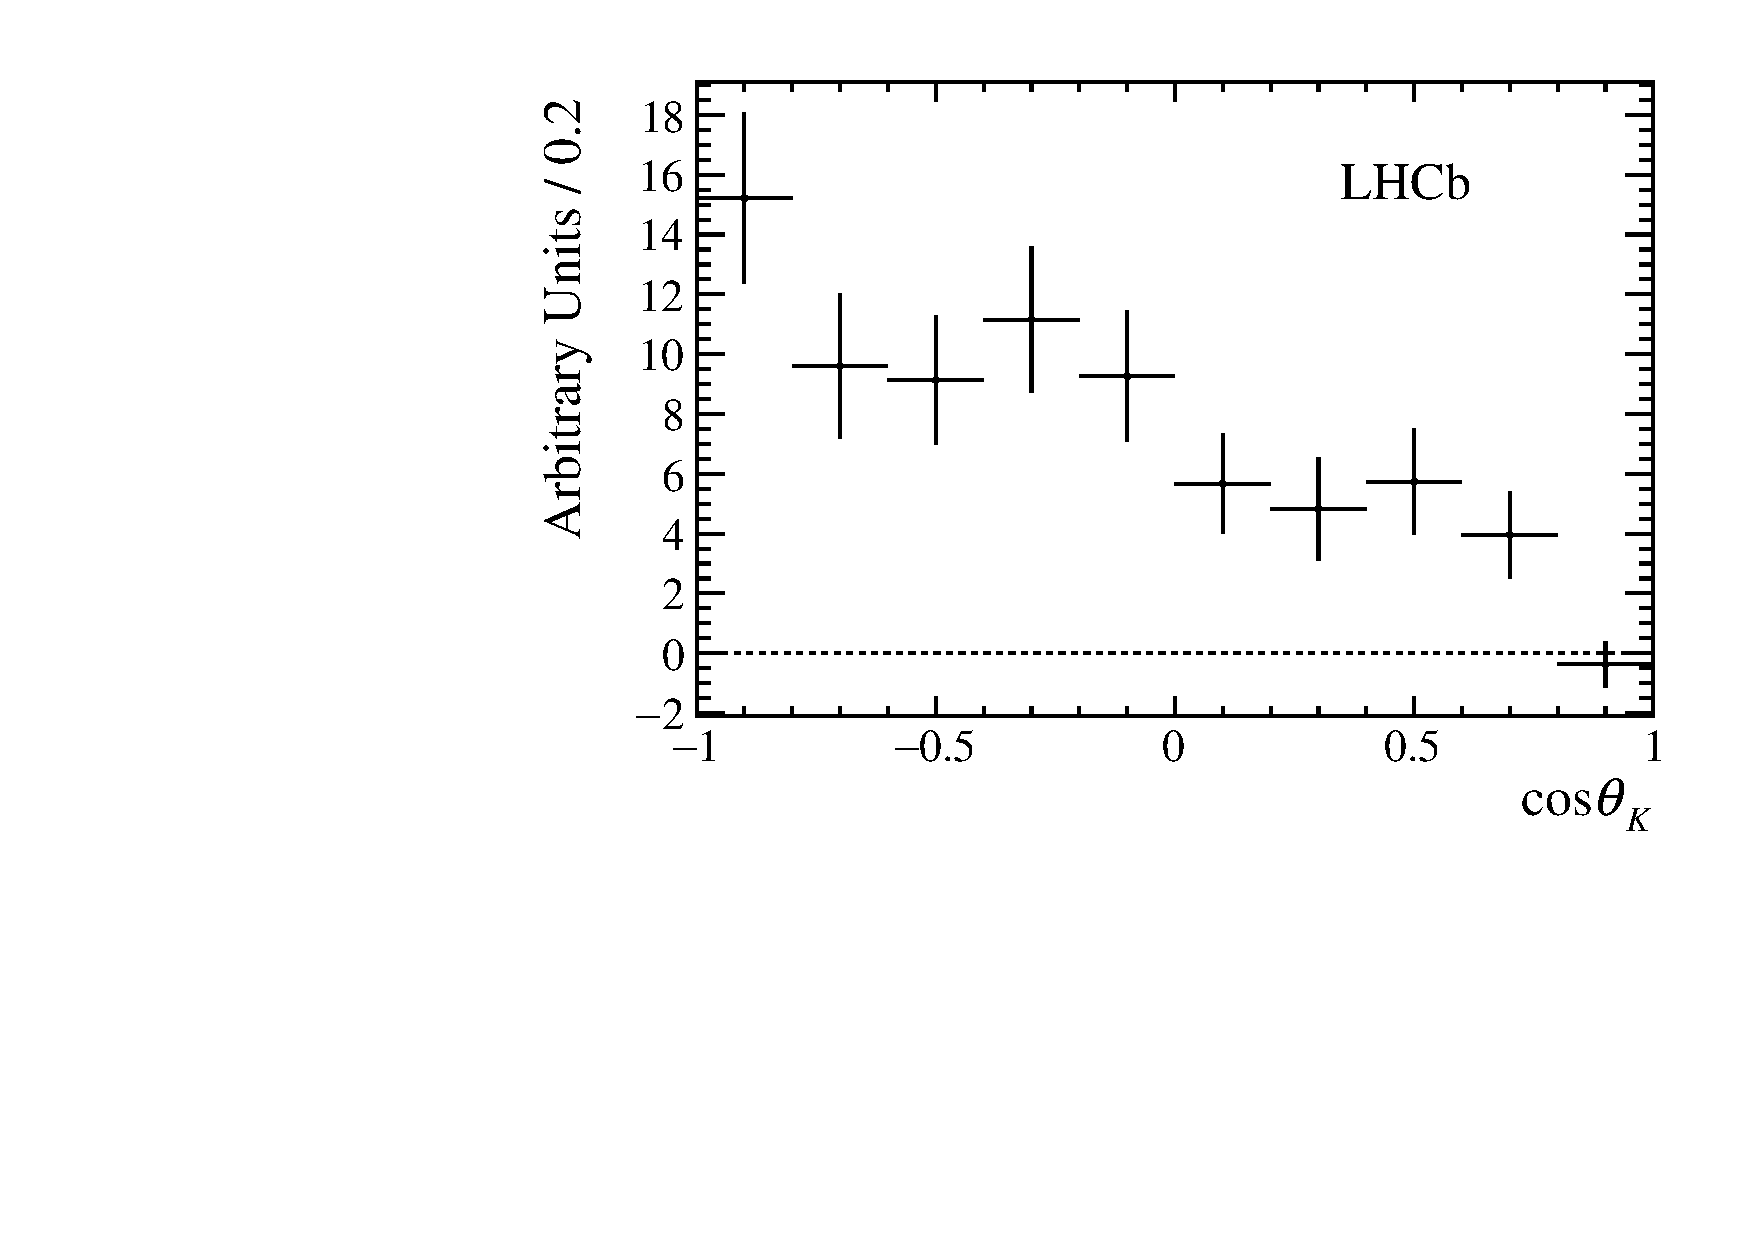
\includegraphics[width=1.0\textwidth]{figs/B2DsKK/helAngle_bin1_sweighted.pdf}
        \caption{$m(\Kp\Km)<1250\mevcc$}
    \end{subfigure}
    \begin{subfigure}[t]{0.49\textwidth}
        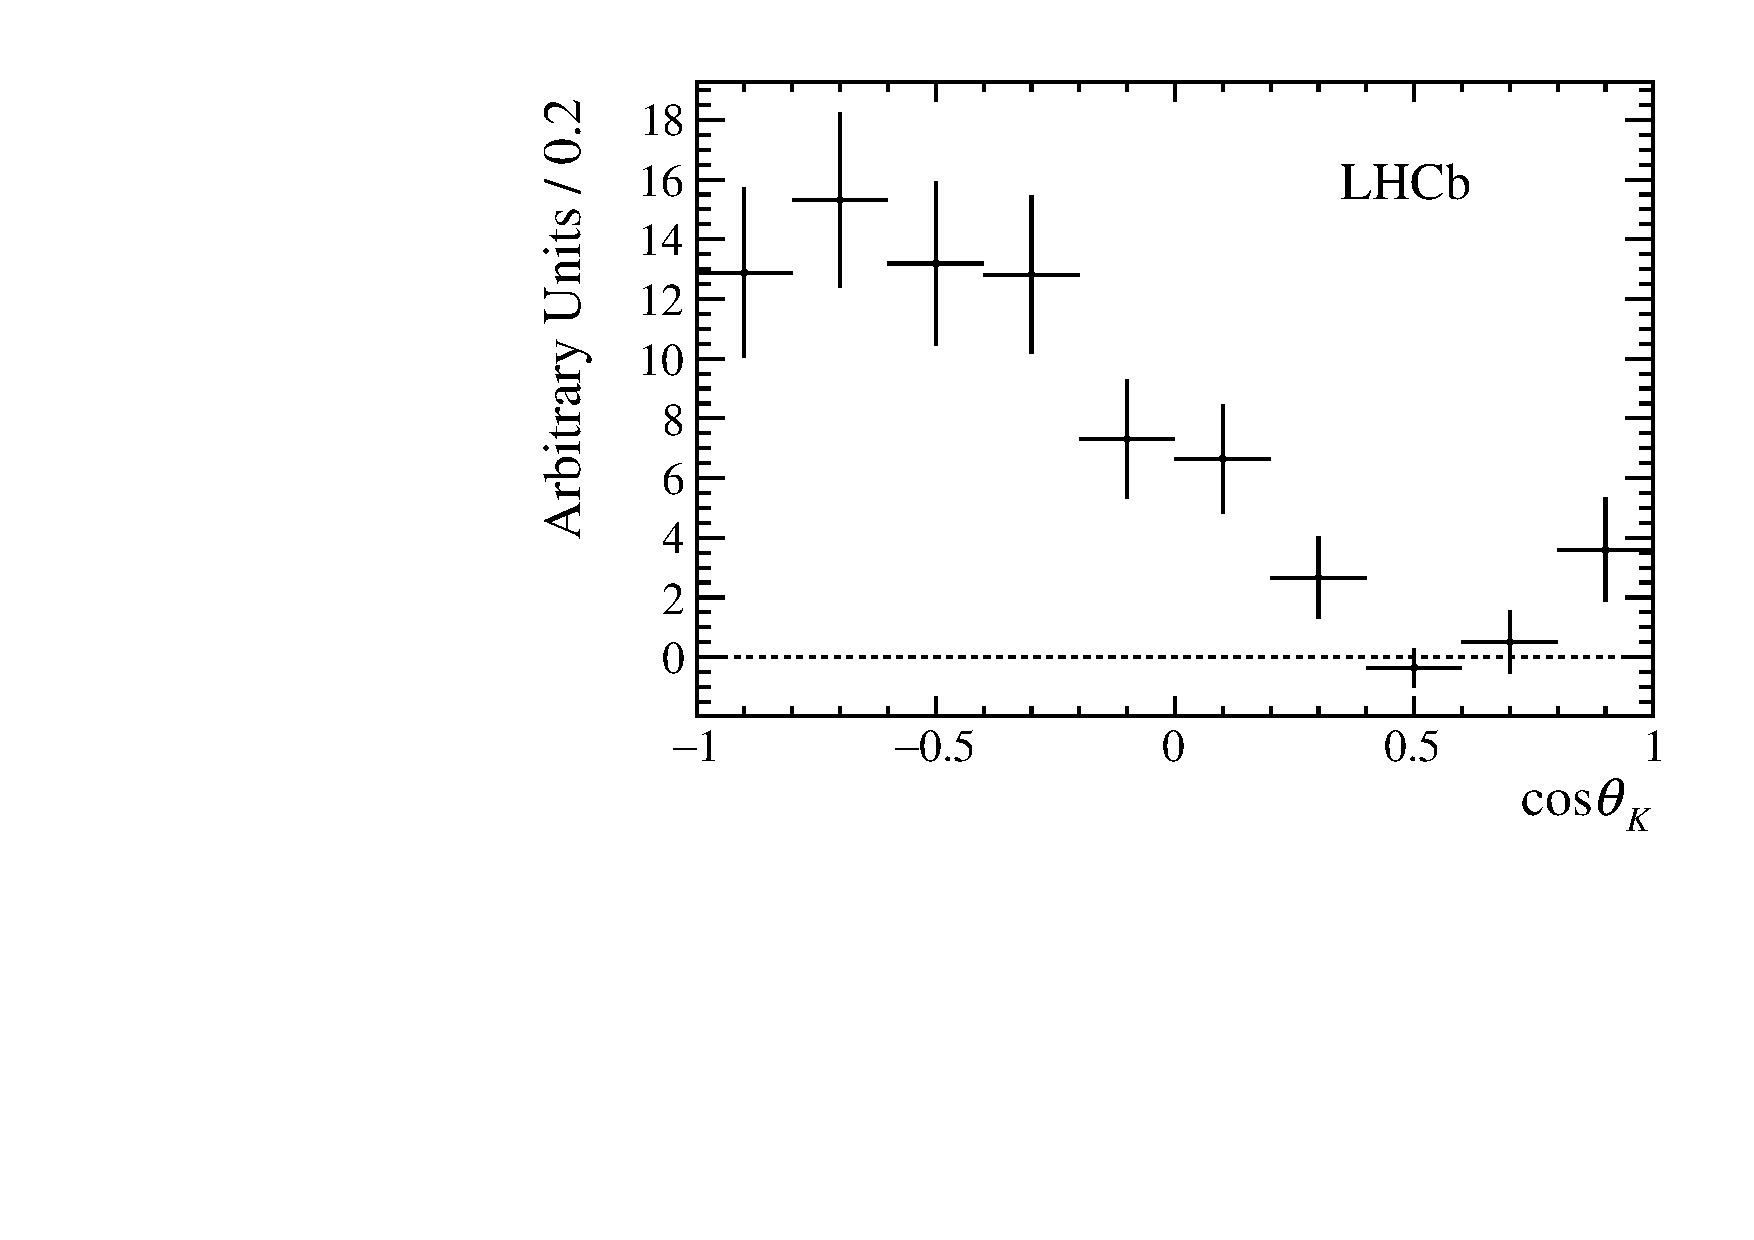
\includegraphics[width=1.0\textwidth]{figs/B2DsKK/helAngle_bin2_sweighted.pdf}
        \caption{$1250<m(\Kp\Km)<1500\mevcc$}
    \end{subfigure}
    \begin{subfigure}[t]{0.49\textwidth}
        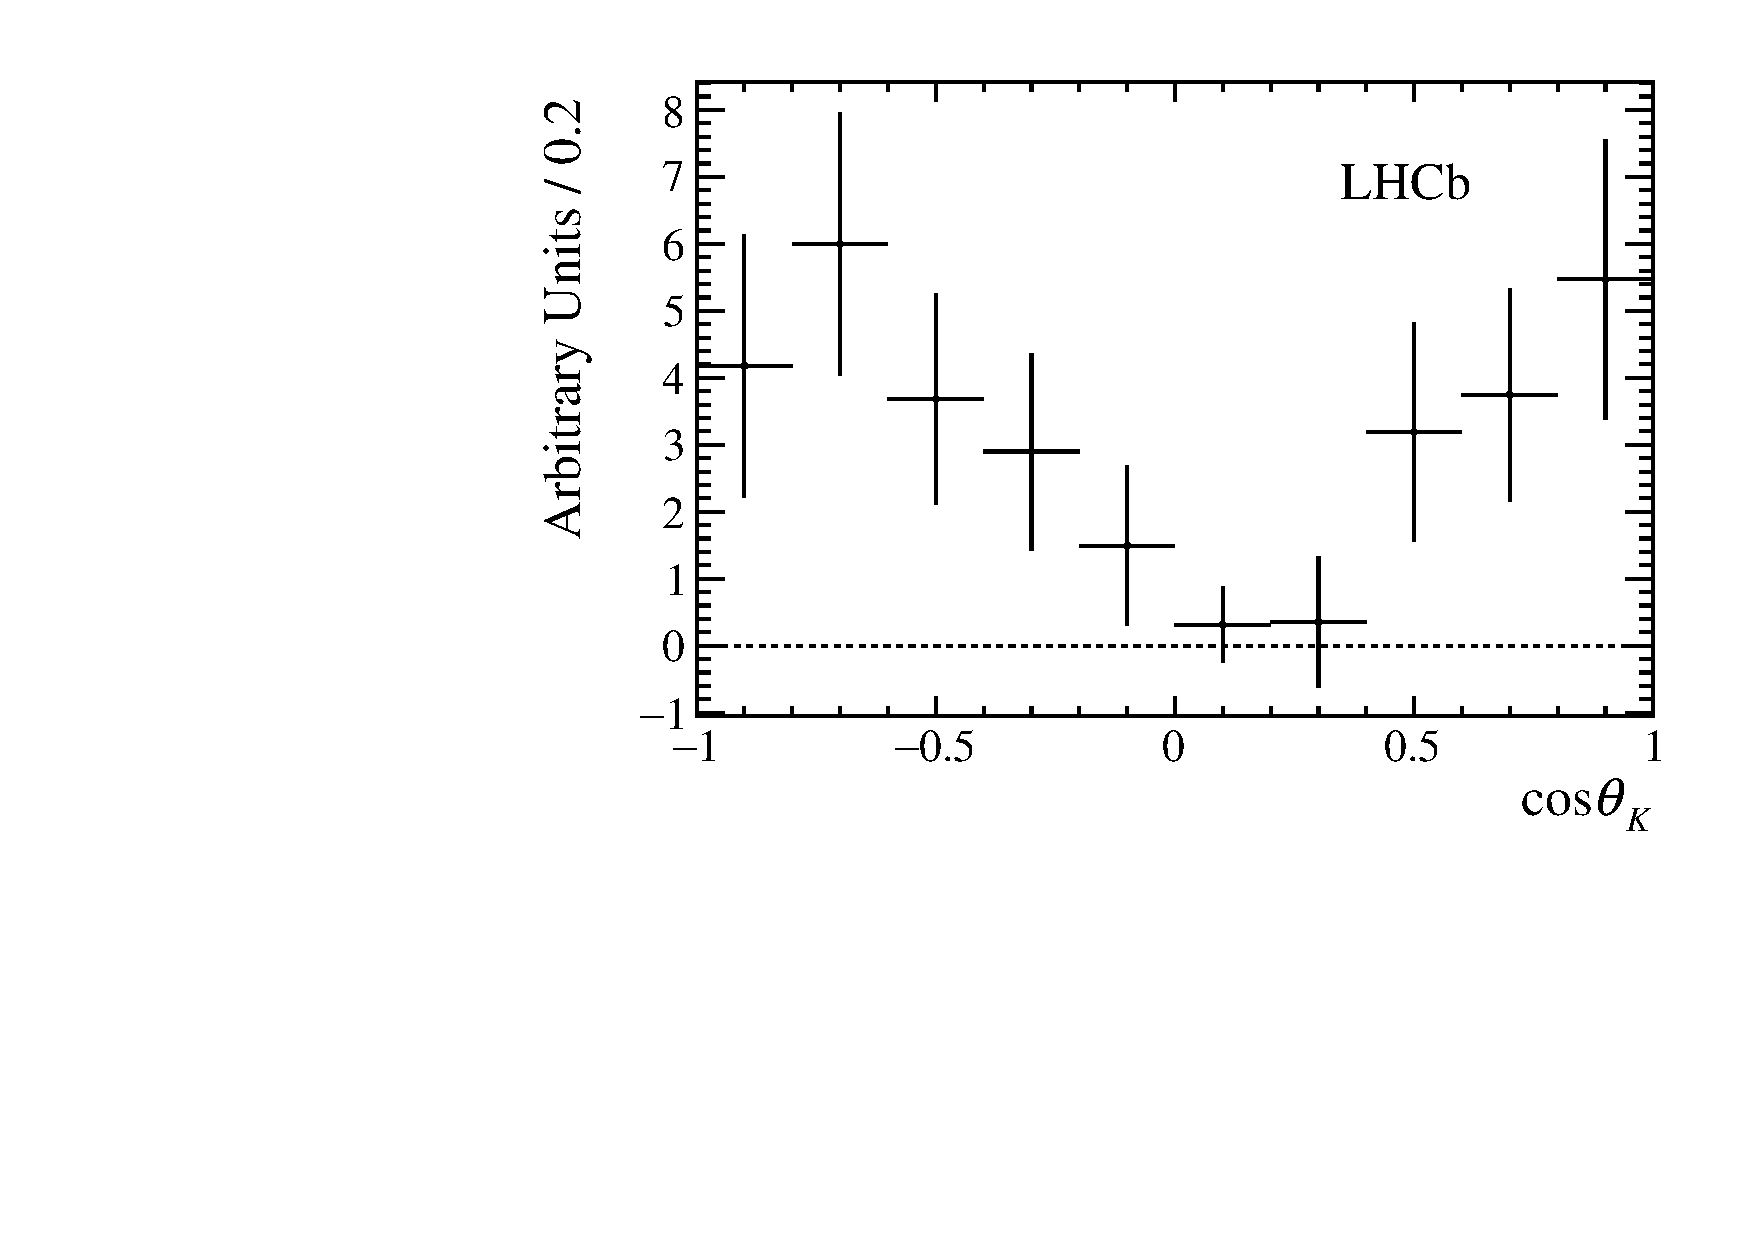
\includegraphics[width=1.0\textwidth]{figs/B2DsKK/helAngle_bin3_sweighted.pdf}
        \caption{$1500<m(\Kp\Km)<1750\mevcc$}
    \end{subfigure}
    \begin{subfigure}[t]{0.49\textwidth}
        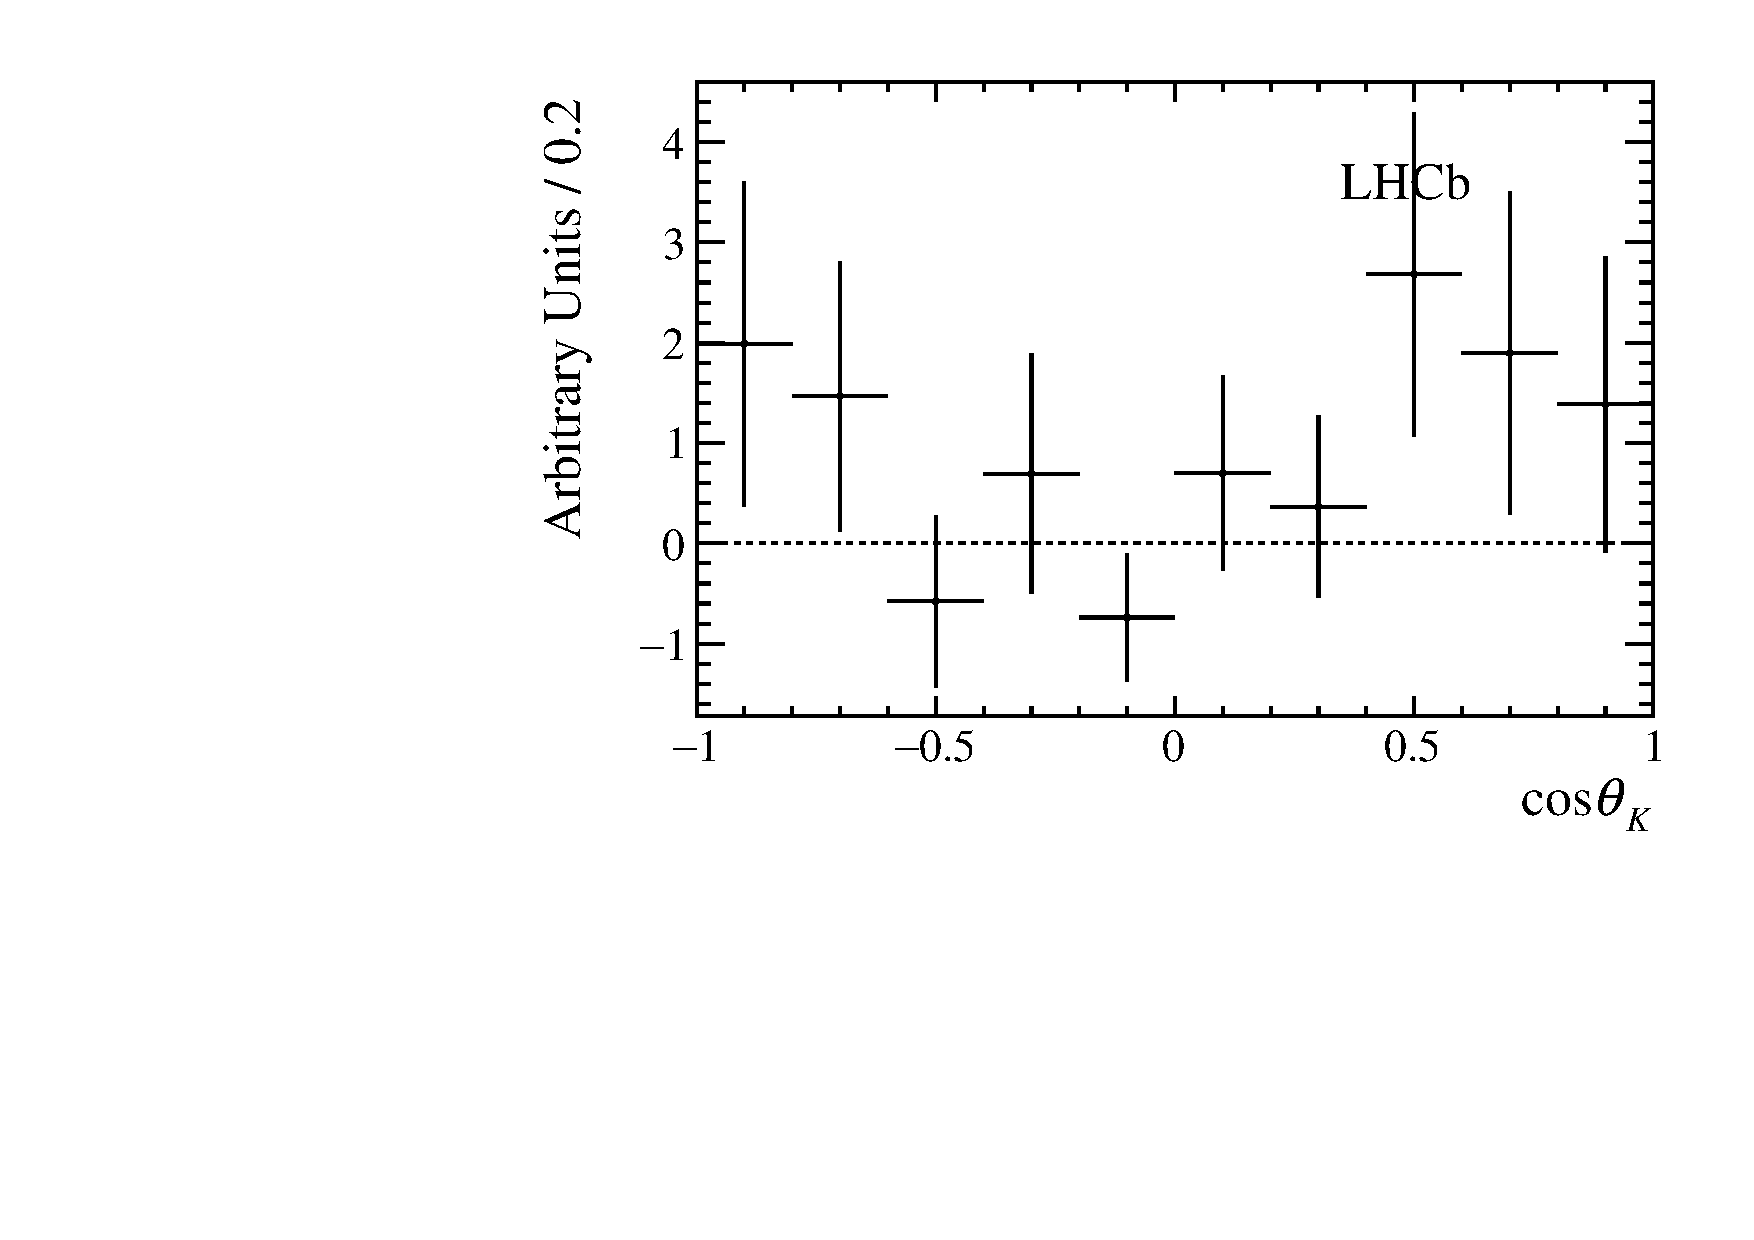
\includegraphics[width=1.0\textwidth]{figs/B2DsKK/helAngle_bin4_sweighted.pdf}
        \caption{$m(\Kp\Km)>1750\mevcc$}
    \end{subfigure}
    \caption{Helicity angle in bins of $m(\Kp\Km)$ mass.}
    \label{fig:B2DsKK_twobodyprojections}
\end{figure}
%%%%%%%%%%%%%%%%%%%%%%%%%%%%%%%%%%%%%%%%%%%%%%%%%%%%%%%%%%


\section{Discussion and outlook}

{\color{Red} Full Amplitude analysis}
